
\documentclass[11pt, a4paper]{article}\usepackage[]{graphicx}\usepackage[]{color}
% maxwidth is the original width if it is less than linewidth
% otherwise use linewidth (to make sure the graphics do not exceed the margin)
\makeatletter
\def\maxwidth{ %
  \ifdim\Gin@nat@width>\linewidth
    \linewidth
  \else
    \Gin@nat@width
  \fi
}
\makeatother

\definecolor{fgcolor}{rgb}{0.345, 0.345, 0.345}
\newcommand{\hlnum}[1]{\textcolor[rgb]{0.686,0.059,0.569}{#1}}%
\newcommand{\hlstr}[1]{\textcolor[rgb]{0.192,0.494,0.8}{#1}}%
\newcommand{\hlcom}[1]{\textcolor[rgb]{0.678,0.584,0.686}{\textit{#1}}}%
\newcommand{\hlopt}[1]{\textcolor[rgb]{0,0,0}{#1}}%
\newcommand{\hlstd}[1]{\textcolor[rgb]{0.345,0.345,0.345}{#1}}%
\newcommand{\hlkwa}[1]{\textcolor[rgb]{0.161,0.373,0.58}{\textbf{#1}}}%
\newcommand{\hlkwb}[1]{\textcolor[rgb]{0.69,0.353,0.396}{#1}}%
\newcommand{\hlkwc}[1]{\textcolor[rgb]{0.333,0.667,0.333}{#1}}%
\newcommand{\hlkwd}[1]{\textcolor[rgb]{0.737,0.353,0.396}{\textbf{#1}}}%
\let\hlipl\hlkwb

\usepackage{framed}
\makeatletter
\newenvironment{kframe}{%
 \def\at@end@of@kframe{}%
 \ifinner\ifhmode%
  \def\at@end@of@kframe{\end{minipage}}%
  \begin{minipage}{\columnwidth}%
 \fi\fi%
 \def\FrameCommand##1{\hskip\@totalleftmargin \hskip-\fboxsep
 \colorbox{shadecolor}{##1}\hskip-\fboxsep
     % There is no \\@totalrightmargin, so:
     \hskip-\linewidth \hskip-\@totalleftmargin \hskip\columnwidth}%
 \MakeFramed {\advance\hsize-\width
   \@totalleftmargin\z@ \linewidth\hsize
   \@setminipage}}%
 {\par\unskip\endMakeFramed%
 \at@end@of@kframe}
\makeatother

\definecolor{shadecolor}{rgb}{.97, .97, .97}
\definecolor{messagecolor}{rgb}{0, 0, 0}
\definecolor{warningcolor}{rgb}{1, 0, 1}
\definecolor{errorcolor}{rgb}{1, 0, 0}
\newenvironment{knitrout}{}{} % an empty environment to be redefined in TeX

\usepackage{alltt}
\usepackage{indentfirst}
\usepackage{verbatim}
\usepackage[vmargin=3cm, hmargin=2cm, headheight=14pt]{geometry}
\usepackage{url}
\usepackage{hyperref}
\usepackage{fancyhdr}
\usepackage{color}
\usepackage{amsmath, amssymb}
\usepackage{longtable}
\usepackage{lscape}
\usepackage{natbib}
\usepackage{xspace}
\usepackage[sc]{mathpazo}
\linespread{1.05} 
\usepackage[scaled]{helvet}
\usepackage[section]{placeins}
\usepackage{booktabs}

\usepackage[font=sf, labelfont={sf}, margin=1cm]{caption}

\usepackage[T1]{fontenc}
\usepackage[latin1]{inputenc}

% =======================================
% Personalized layout
\newcommand{\name}{Xijin Chen}
\newcommand{\mail}{xijin.chen@uzh.ch}
\newcommand{\versiondate}{\today}
\newcommand{\client}{Thomas Radtke} 
\newcommand{\clinic}{EBPI} % umlaute: \"a = ä, specify precisely, not just USZ 
\newcommand{\supervisor}{Julia Braun} 
\newcommand{\projecttitle}{What are predictors of long-term work participation in patients with cystic fibrosis undergoing lung transplantation?}
\newcommand{\subtitle}{STA490: Statistical Consulting \\[.15cm]
  {\Large Leonhard Held} \\[.25cm] 
   {\large EBPI, Department of Biostatistics}}

% =======================================

\newcommand{\web}{www.biostat.uzh.ch}
\newcommand{\grp}{Master Program in Biostatistics}
\newcommand{\inst}{University of Zurich}
\newcommand{\img}{
\includegraphics[height=17mm, width = 53mm]{uzh_logo_e_pos}}
\newcommand{\of}{of\xspace}

\newcommand{\HRule}{\rule{\linewidth}{0.5mm}}
\newcommand{\mytitle}[3]{
\begin{center}
\vspace*{-2.1cm}

\HRule

\vspace*{0.4cm}

\begin{minipage}{0.4\textwidth}
\thispagestyle{empty}
\begin{flushleft}
\hspace*{1cm}\img
\end{flushleft}
\end{minipage}
\begin{minipage}{0.59\textwidth}
\begin{flushleft} \large
    \hspace*{3.8cm} \textsf{\grp} \\
    \hspace*{3.8cm} \href{http://\web}{\textsf{\emph{\web}}}
\end{flushleft}
\end{minipage}

\vspace*{0.4cm} \HRule

\bigskip

\textsf{\LARGE #2} \vspace*{0.5cm}

\large{#1}

\medskip

\large{\name \ (\textit{\mail})}

\medskip

Version \of \versiondate

\end{center}

\medskip
}


% Headers and footers
\fancypagestyle{standard}{
\fancyhf{}
\renewcommand{\footrulewidth}{0.4pt}
\fancyfoot[c]{\thepage}
\fancyfoot[l]{\textsf{\name}, \href{\mail}{\textsf{\emph{\mail}}}}
\fancyfoot[r]{\textsf{\versiondate}}
\renewcommand{\headrulewidth}{0.4pt}
\fancyhead[c]{}
\fancyhead[l]{\textsf{\grp}}
\fancyhead[r]{\textsf{\inst}}
}

% =======================================
%bibliography
\bibliographystyle{ims}



% =======================================

% =======================================
% my latex commands
\newcommand{\prog}[1]{\textsf{#1}}
\newcommand{\pkg}[1]{\texttt{#1}}
\IfFileExists{upquote.sty}{\usepackage{upquote}}{}
\begin{document}


\pagestyle{standard}
\mytitle{\projecttitle\\[.25cm] Analysis for \client, \clinic \\[.25cm] Supervision by \supervisor}{\subtitle}

\bigskip

% =======Some Initial settings for R==============

%========End of Initial Settings for R============








% =======================================
\section{Abstract} \label{sec:abstract}
% =======================================

\textit{Background:}

Cystic Fibrosis is a type of dysfunction of secretory glands, which affects lungs, digestive system and sweat glands. Lung transplantation is a standard of care for advanced lung diseases. Cystic fibrosis patients may be able to return to work after lung transplantation because of prolonged survival and improved quality of life. The aim of this study is to identify the predictors for long-term work participation in cystic fibrosis patients undergoing a lung transplant.


\textit{Methods:}

This retrospective study included 99 cystic fibrosis patients having received lung transplantation between January 1996 and December 2016 at University Hospital Zurich. Factors describing patients' basic characteristics (age, sex, Body Mass Index, Six-minute Walk Test Distance, education, relationship status, living status and pre-employment status) were retrieved from the patients' charts. After evaluation tests, all of those 99 cystic fibrosis patients entried in the waiting list to wait for a healthy lung. After the lung transplantation, the follow-up time was divided into five periods: within one year, one to three years, three to five years, five to ten years and more than ten years after lung transplantation. Lung recipients may go through some rejection, infection and transplantation-related complications during the follow-up time.

To evaluate the work participation after lung transplantation, we investigated both work status and average of work percentage at each time period: one year, three years, five years, ten years after lung transplantation and the end of the study.

Predictors for work status at each time point were identified by logistic regression. Predictors for work percentage at each time point were identified by linear regression. Based on the results from 'simple' regression from the measurements on each time point, generalized linear mixed models and linear mixed models were used for longitudinal data analysis to identify predictors for long-term work participation.

The criterion for model selection in this study is the Bayesian Information Criterion (BIC).

\textit{Results:}

When focusing on each specific time point after lung-transplantation, the results from logistic regression show that there are two possible time-independent predictors for work status after lung transplantation: \textit{Pre-employment} and \textit{Education}. One to three years after lung transplantation, the odds ratio for \textit{Pre-employment} is 11.19, with 95\% confidence interval from 3.67 to 42.71. It shows very strong evidence for the effect on work status. The odds ratio for \textit{Education} is 5.34, (95\% confidence interval from 1.22 to 37.82), showing moderate evidence for its effect on work status.   

The results from linear regression show that the only predictor for work percentage after lung transplantation is \textit{Pre-employment}. The strength of evidence varies between time periods.


From the results of longitudinal data analysis, besides \textit{Pre-employment} and \textit{Education}, there are some time-dependent factors that may have an effect on work participation.

From the results of the generalized linear mixed-effects model, \textit{CLAD} (Chronic Lung Allograft Dysfunction) would have a negative effect on the post-transplantation work status. The odds ratio is 0.64, 95\% confidence interval from 0.15 to 2.40, showing strong evidence of the negative effect on the work status after lung transplantation.

From the result of the linear mixed-effects model, \textit{Kidney-Dialysis} would have a negative effect on the post-transplantation work percentage. The coefficient is -18.69, 95\% confidence interval  from -31.80 to -5.59, with moderate evidence for the association between \textit{Kidney-Dialysis} and long-term work percentage.


\textit{Conclusions:}

We determined time-independent factor \textit{Pre-employment} and \textit{Education} as the factors that would have an effect on both work status and work percentage after lung transplantation. Besides time-independent factor, we decided to use \textit{CLAD} as another predictor for the long-term work status after transplantation. \textit{Kidney-Dialysis} is the predictor that we chose for the long-term work percentage after transplantation.

In a word, patients who were employed, and with academic education before transplantation would be more likely to return to work. Chronic Lung Allograft Dysfunction is a kind of limitation for the cystic fibrosis patients to return to work after transplantation. Patients who had kidney transplantation or dialysis after transplantation, would work less than the others without renal dysfunctions.

\vspace{2cm}

% =======================================
\section{Introduction} \label{sec:intro}
% =======================================

%%%%%%%%%%%%%%%%%%%%%%%%%%%%%%%%%%%%%%%%%%%%%%%%%%%%%%%%%%%%%%%%%%%%%%%%%%%%%%%%%
% 1.LTx and CF,work participation
\subsection*{Cystic fibrosis, lung transplantation and work participation} 

Cystic fibrosis (CF) is a genetic disorder passed down from generations to generations. It is caused by the presence of mutations in both copies of the gene for cystic fibrosis transmembrane conductance regulator (CFTR) protein. Those with a single working copy are carriers and otherwise mostly unaffected When the protein is not working correctly, it's unable to help move chloride, a component of salt, to the cell surface. Without chloride attracting water to the cell surface, the mucus in various organs becomes thick and sticky. In the lungs, mucus clogs the airways and traps germs, e.g. bacteria, leading to infections, inflammation, respiratory failure, and other complications. Cystic fibrosis patients frequently can not work due to cancers of the digestive tract, diabetes, heart failure, kidney problems and lung infections.
  
There is currently no cure for cystic fibrosis since it is inherited, but several kinds of treatments can ease symptoms and reduce complications. Those treatments can help prevent and control infections that occur in the lungs, remove and loosen mucus from the lungs, treat, prevent intestinal blockage and provide adequate nutrition as well. Currently, there are many options for treatment, e.g. medication, chest physical therapy, pulmonary rehabilitation and surgery. 

Lung transplantation (LTx) has become the standard of care for patients with end-stage chronic respiratory failure, which is necessary when medical management alone can no longer maintain lung health and physical function \citep{derhovanessian2018chronic}. Lung transplantation is a surgery removing a diseased lung and replacing it with a healthy lung from a donor. Transplantation can be divided into two types, cadaveric transplantation from deceased organ donors and living transplant from part of one of the lungs form healthy adults. More than 6,400 lung transplantations have been performed since the first successful operations in the early 1980s \citep{hosenpud1997registry}. 

Patients underwent evaluation tests as a preparation process before lung transplantation, including a variety of medical tests that provide complete information about overall health of patients. Those medical tests aim at helping the lung transplant team to identify any potential problem before the transplant surgery and avoid potential complications after the surgery. From a practical perspective, patient selection involves analysis of standard investigations designed to identify comorbidities that may increase risk, and to balance those against likely outcomes. After the evaluation tests, patients would entry in the waiting list before transplantation.

Patients' work participation is a common clinical quality indicator being used to monitor the performance of healthcare services \citep{choong2017linking}, which helps to assess the quality of care, identify and prioritize areas for improvement \citep{crampton2004makes}, \citep{mainz2003defining}. In addition to life expectancy, this simple measure of health outcome can also reflect the reduction of disability and improvement of health-related quality of life (HRQoL). As indicated in \cite{tumin2016attained} and \cite{suhling2015employment}, lung transplantation can alleviate some physiological barriers to employment. Therefore, work participation can be used as an indicator for long-term performance after lung transformation \citep{krivchenia2016long}. 

%%%%%%%%%%%%%%%%%%%%%%%%%%%%%%%%%%%%%%%%%%%%%%%%%%%%%%%%%%%%%%%%%%%%%%%%%%%%%%%%%
% 2.Recent studies
\subsection*{Evidence from recent studies} 

There is a great number of references related to work participation after organ transplantation. In the analysis of solid organ transplantation, there is a list of factors being positively associated with returning to work after organ transplantation. Being employed before transplantation \citep{hunt1996effect, nour2015factors, white2011factors}. High level educated patients, male patients would be more likely to return to work after organ transplantation from the results in \cite{vieux2018predictors}.

In terms of lung transplantation for lung diseases in cystic fibrosis patients, better outcomes are limited by a list of factors \citep{targett2013employment, taylor2013longitudinal, laborde2012employment}. As shown across studies \cite{huda2015employment, eppenberger2015back, aaberg2016prolonging, matas1996employment}, pre-employment is the most consistent and dominant predictor for work participation. There is a strong positive association between the pre-employment and post work status. From the study \cite{krivchenia2016long}, lack of work history before lung transplantation was identified as a barrier to post-transplant employment in cystic fibrosis patients. 
The result of influence of education levels should not be ignored by \cite{krivchenia2016long}. In this study for lung transplantation for cystic fibrosis patients, the level of education was associated with the work participation  after lung transplantation. From \cite{laborde2012employment}, not only education, but also best predicted FEV1(\%) showed a significant effect on the post-transplantation work status in multivariate analysis.

%%%%%%%%%%%%%%%%%%%%%%%%%%%%%%%%%%%%%%%%%%%%%%%%%%%%%%%%%%%%%%%%%%%%%%%%%%%%%%%%%
%4.factors that we are interested with
\subsection*{Possible predictors in our study} 

There is also a list of possible predictors in our study. Patient attributes and physical characteristics are common basic information that can be retrieved or tested. Evidence shows that clinical decision making varies according to patients \citep{lutfey2008patient}, as characteristics provide important information about prior probability that a given patient will experience a given condition or problem. 

The level of education can tell us about the possible post-transplantation work participation to some extent. Well-educated patients are more likely to go into skilled labor as opposed to manual work. Therefore, highly-educated patients would be more likely to return to work. 

Measurements like body mass index, six-minute walk test distance \citep{tuppin2008predictive}, reflect physical functions of patients, which are directly related to the performance after lung transplantation. It varies greatly, depending on age, blood type, the status of the lung of patients and the availability of a donor lung that is a good match. People who are unable to wait may be considered for lung transplant from a living donor. Up to 25 to 41 \% of cystic fibrosis patients have died while awaiting a healthy lung as illustrated by \cite{vizza2000outcome}, \cite{sharples1993prognosis}, \cite{stanchina2002association} and \cite{ciriaco1995analysis}. Therefore, too long waiting time may impede the patient's utility gain from the treatment. 


A list of risks after a lung transplantation could also bring some barriers to work participation. Rejection is a normal body reaction to a foreign object or tissue. When an organ is transplanted into a person's body, their immune system sees it as a threat and attacks the organ. From the study \cite{derhovanessian2018chronic}, main limitation to better long-term survival after lung transplantation is chronic lung allograft dysfunction (CLAD). 

After solid organ transplantation, the risk of cancer in the digestive tract is elevated 2-4 fold compared with population controls. The high risks for cancer are associated with viral infections, including Mb, Hodgkin and non-Hodgkin lymphoma (NHL) (caused by Epstein Barr virus [EBV]), anogenital cancer (human papillomavirus), and liver cancer (hepatitis C and B virus), but also for other malignancies such as lung, kidney, skin, and thyroid cancer.

%start
Better management of medical complications may lead to improved long-term outcomes. Improvements in surgical techniques, lung preservation, immunosuppression, and management of infections have influenced the improvements in mortality by \cite{trulock2007registry}. 

Renal dysfunction is one of the most common long-term complications of lung transplantation and may have an effect on the post-transplantation work participation, with an incidence of 25.5\% at 1 year after transplant and 37.8 at 5 years after transplant from \cite{trulock2007registry}. The development of chronic renal failure increases the risk of death by four to five fold in patients who have undergone lung transplant \citep{ojo2003chronic}. The progression of chronic renal failure ultimately leads to renal replacement therapy in the form of dialysis or renal transplantation. 

Pulmonary function test results (forced expiratory volume in one second [FEV1]), were expressed as the percentage of the predicted value and the best values achieved after the lung transplantation. FEV1, as a result of breathing test, is normally used to show the severity of chronic obstructive pulmonary disease. The measurement of FEV1 for a given patient is compared to reference values. The reference value is based on healthy individuals with normal lung function and it shows the values that would be expected for someone of the same sex, age and height. If the predicted values of patients are within 80\% of the reference value, the results are considered normal. As indicated in \cite{cicutto2004factors}, the value of FEV1 count for work participation.

Therefore, our study would investigate all the possible predictors listed above to identify the predictors for long-term work participation in cystic fibrosis patients after lung transplantation.

%%%%%%%%%%%%%%%%%%%%%%%%%%%%%%%%%%%%%%%%%%%%%%%%%%%%%%%%%%%%%%%%%%%%%%%%%%%%%%%%%
%6.the specific point of our study

\subsection*{Aim of our study} 

In an attempt to characterize the impact of lung transplantation on the long-term work participation for cystic fibrosis patients, the aim of our study is to identify the predictors for long-term work participation after lung transplantation.

To our acknowledgement, there is no research about the longitudinal data analysis with respect to both work status and work percentage after lung transplantation. 

Our study identified the predictors not only for work status, but also for work percentage, as a compensation analysis. After the conventional analysis at each time point, our study took the effect of time-dependent factors and time into consideration and analyzed outcomes for all time periods by longitudinal analysis. Finally, identifying the predictors for long-term work participation among cystic fibrosis patients.


 
\vspace{1cm}
% =======================================
\section{Research Questions} \label{sec:questions}
% =======================================
\begin{enumerate}
    \item What are the predictors for work status in cystic fibrosis patients after lung transplantation?
    \item What are the predictors for work percentage in cystic fibrosis patients after lung transplantation?
\end{enumerate}
\vspace{1cm}
% =======================================
\section{Methods} \label{sec:methods}
% =======================================

% =======================================
\subsection*{Study Design} \label{subsec:design}
% =======================================
\vspace{0.5cm}
\subsubsection*{Type of study}
Retrospective, single center study in the University Hospital Zurich.

\vspace{0.5cm}
\subsubsection*{Study population}
The study population is  99 cystic fibrosis patients receiving lung transplantation, from January 1996 to December 2016.

\vspace{0.5cm}
\subsubsection*{Data collection} 
\label{sec:datacollect}
Social-demographic factors about the basic information of patients (age, sex, education, relationship status, BMI, living status, six-minute walk distance and pre-employment status) were recorded before the transplantation. Among those factors, education was dichotomized into academic or non-academic. Relationship status was dichotomized into single or divorced versus with relationship or married/engaged. Living status was dichotomized into alone and not alone. Pre-employment status were indicated whether the patient was employed or not before the lung transplantation. 

The six-minute walk test (6MWD) measured the distance a patient was able to walk over a total of six minutes on a hard, flat surface. The measurement was a performance-based measure of functional exercise capacity. Body Mass Index was calculated based on the weight and height of patients.


All of those 99 cystic fibrosis patients had finished evaluation tests. The date for waiting list and lung transplantation were recorded, which were needed for the waiting time. The bio-medical factor waiting time was transformed into weeks, unlike the dichotomy for waiting time \cite{laborde2012employment}, to get more accurate result of the influence of waiting time on post-transplantation work participation. 

Observations were obtained at five time points: one year, three years, five years, ten years after lung transplantation and at the end of the study. The best FEV1(\%) out of all those repeated measurements for our patients was used. Besides, we got the exact time for chronic lung allograft dysfunction (CLAD), Kidney transplant, dialysis and cancer if these events occurred.

Work participation, were evaluated in two ways, work status and the average of work percentage between two separate time points of measurements after lung transplantation. Post-transplant work status was divided into not work or work after lung transplantation, post-transplant work percentage was from 0 to 100(\%).
  


\vspace{0.5cm}
% =======================================
\subsection*{Statistical Analysis} \label{subsec:statmethods}
% =======================================
\subsubsection*{Data preparation}

We used the difference between the date of putting on the waiting list and date of lung transplantation for waiting time of each patient, the differences were transformed into weeks.

Similarly, we calculated the difference between the date of events and date of lung transplantation,  and then compared the difference with the date of each time point: one year, three years, five years, ten years after lung transplantation and at the end of the study. The results of comparison were used to create binary variables for each time periods. Therefore, those time-varying variables, increased monotonously with time.

This time-varying variable takes two events into consideration: kidney transplantation and dialysis. Both of them are management for the complication of renal dysfunction, so we created one binary variable to reflect the effect of renal dysfunction on the work participation after lung transplantation.

work status and work participation, and those three time-varying variables were measured repeatedly at several time points, we transformed whole dataset into long-format data for the preparation of the longitudinal data analysis.

Since the period of waiting time vary a lot for each patient, not all of those 99 patients would go through the
whole study period (20 years). Therefore, those 99 patients may have different number of repeated measurements. Some of those patients would have measurements for both outcomes and time-dependent factors for all five time points, while others may have only 1.

\vspace{0.5cm}
\subsubsection*{Statistical model}

For work status after transplantation, logistic regressions were used for different time periods. Based on the result of initial analysis, generalized linear mixed effect model was used for longitudinal data analysis.

For work percentage after transplantation, simple linear regressions were used for different time periods. Based on the result of initial analysis, linear mixed effect model was  used for longitudinal data analysis.


\vspace{0.5cm}
\subsubsection*{Visualization methods}
We used a great number of visualization methods in our study:

\begin{enumerate}
\item Boxplot: Age, Sex, Living status, Relationship status, Post-transplantation work percentage.

\itemn Histogram: Waiting time, BMI and Best FEV1(\%).

\item Jitter plot: Two by two table visualization.

\item Heatmap: The distribution of time-varying variables.

\item Likert: Post-transplantation work status.

\item Barplot: Number of repeated measurement for patients.

\end{enumerate}
\vspace{0.5cm}
\subsubsection*{Implementation}

We used a great number of packages for implementation.

\begin{enumerate}
\item Data cleaning: \textit{zoo} for the date variables, \textit{stringr} for vectorization of characteristics variables and \textit{tidyr} for gathering values.


\item Table making: \textit{tableone}, \textit{xtable}, \textit{reporttools} and related function in \textit {biostatUZH} from EBPI.

\item Plot: \textit{likert}, \textit{ggplot2}, \textit{ggpubr},\textit{superheat}, \textit{RColorBrewer} for colors for plots, \textit{ggbeeswarm} and \textit{sjPlot}, 

\item Longitudinal data analysis: \textit{lme4}, \textit{lmerTest}.

\end{enumerate}

\clearpage


\vspace{2cm}
% =======================================
\section{Data Description} \label{sec:Description}
% =======================================
% =======================================
\subsection*{Data description for possible predictors} \label{subsec:factors}
% =======================================
As is shown in section \ref{sec:datacollect}, factors were collected before lung transformation or after transformation. We have repeated measurements on those factors we collected from different time points. However, not all of those post-transplantation factors would change with time. \textit{Best FEV1\% pred} is a factor that have repeated measurements, but being time-independent.

We classify the types of predictors based on the whether they change with time, in other words, time-dependent factors and time-independent factors.

\vspace{1cm}
% =======================================
\subsubsection*{Description for time-independent factors}\label{subsubsec:time_ind}
% =======================================
\begin{table}[ht]
\centering

\begin{tabular}{lll}
\toprule
  & level & Overall\\
\midrule
n &  & 99\\
Age (mean (SD)) &  & 35.02 (10.30)\\
BMI (mean (SD)) &  & 18.32 (3.15)\\
6MWD (mean (SD)) &  & 394.27 (108.03)\\
Best FEV1 pred (mean (SD)) &  & 92.67 (17.84)\\
\addlinespace
Waiting time (mean (SD)) &  & 41.83 (38.87)\\
Sex (\%) & Female & 49 (49.5)\\
 & Male & 50 (50.5)\\
Education (\%) & Non-academic & 78 (78.8)\\
 & Academic & 21 (21.2)\\
\addlinespace
Relationship (\%) & Not single & 31 (32.0)\\
 & Single & 66 (68.0)\\
Living (\%) & Not alone & 79 (81.4)\\
 & Alone & 18 (18.6)\\
Pre-employment (\%) & Non-employed & 52 (52.5)\\
\addlinespace
 & Employed & 47 (47.5)\\
\bottomrule
\end{tabular}


\caption{Time-independent factors}\label{tab:tab1}
\end{table}

The main characteristics of the 99 patients are listed in table \ref{tab:tab1}. The mean age of our study population is 35 years old. 

Most of the patients had non-academic education 
(78.79\%), 
living not alone 
(81.44\%) 
and being single 
(31.96\%). With regard to sex, there is a balance in this study population. 

The mean of the waiting time for a healthy lung in this study population is about 
42 weeks 
(9.8 months). There is high variance of the waiting time among all those patients.

\begin{figure}[ht]
\centering
\begin{knitrout}
\definecolor{shadecolor}{rgb}{0.969, 0.969, 0.969}\color{fgcolor}
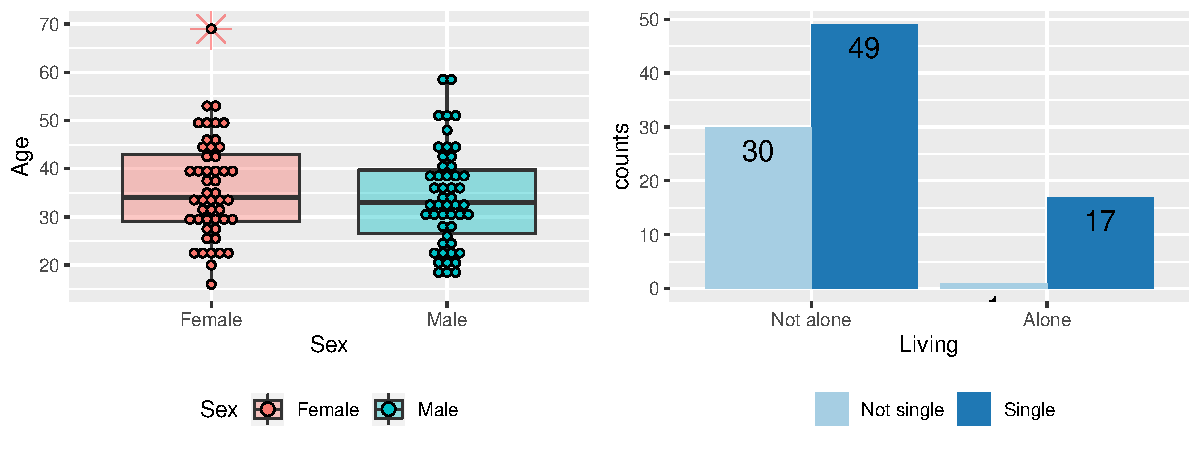
\includegraphics[width=\maxwidth]{plots/pagesex-1} 

\end{knitrout}
\caption{Distributions of population with respect to Sex, Age, Living and Relationship Status}\label{fig:fig1}
\end{figure}

Figure \ref{fig:fig1} shows that for male and female patients, the distribution of age are very similar. The mean of age in these two groups, are both around 35 years old. The age of half of the patients range from 28 to 42 years old. There is one outlier, who was much older than the rest of patients. This is an individual case with age of 69 years old. The distribution of age of patients illustrate the fact that too old patients would not be proper candidates for lung transplantation.


As for relation status and living status, there is an obvious imbalance. Much more patients were living alone, and the proportion of single patients was twice as large as the proportion of the not single group.


\begin{figure}[ht]
\begin{knitrout}
\definecolor{shadecolor}{rgb}{0.969, 0.969, 0.969}\color{fgcolor}
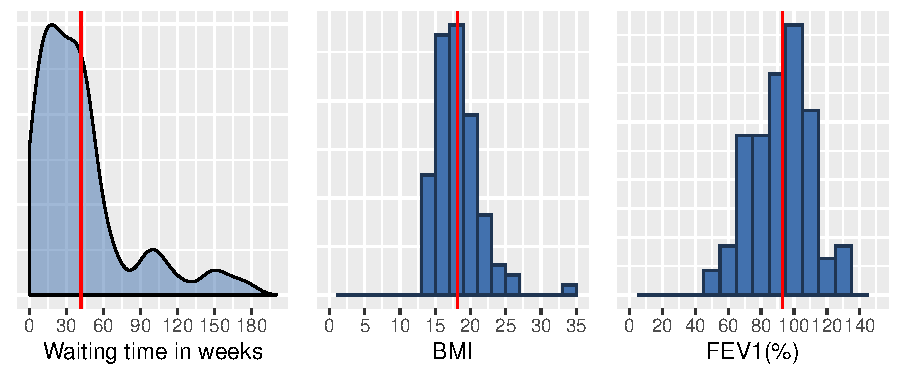
\includegraphics[width=\maxwidth]{plots/pcontin-1} 

\end{knitrout}
\caption{Distributions of some characteristics of physical functions}\label{fig:fig2}
\end{figure}

Figure \ref{fig:fig2} shows distributions of some characteristics of physical functions and waiting time. the longest waiting time for patients were about 177 weeks, while the lowest waiting time is very close to 0. In total, the majority of patients waited no longer than 60 weeks in this study.

As shown in figure \ref{fig:fig2}, the mean of BMI is about 18.32 $kg/m^2$, the distribution of BMI tells us that majority of those 99 patients in this study population had lower than 25$kg/m^2$ BMI, indicating the underweight problem of cystic fibrosis patients, as a result of dysfunction of digestive system problems.
\clearpage


\begin{figure}[!ht]
\centering
\begin{knitrout}
\definecolor{shadecolor}{rgb}{0.969, 0.969, 0.969}\color{fgcolor}
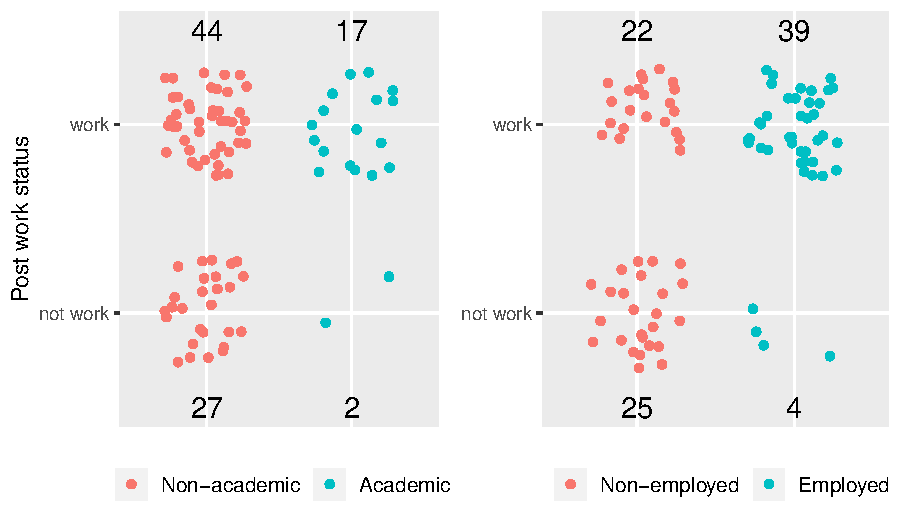
\includegraphics[width=\maxwidth]{plots/passos_educationplot-1} 

\end{knitrout}
\caption{Distributions for Education and Pre-employment with respect to work status three years after LTx}\label{fig:fig3}
\end{figure}



We picked measurements from one specific time point to show the distribution of outcomes. The left figure in figure \ref{fig:fig3} shows that there are only 2 cases, with academic education background, not working after lung transplantation.  

Similarly, the right side in figure \ref{fig:fig3} illustrates that there are only 4 pre-employed cases, not working after lung transplantation.

The total number in both plots are not corresponding to what is shown in table \ref{tab:tab1}, since there are some patients that we had no information for the work status one to three years after lung transplantation.

Figure \ref{fig:fig3} indicates that there may be some relations between education or pre-employment and post-transplantation work status. 



% =======================================
\subsubsection*{Description for time-dependent factors}\label{subsubsec:time_dep}
% =======================================
% latex table generated in R 3.5.2 by xtable 1.8-4 package
% Thu Oct 10 20:45:47 2019
\begin{table}[ht]
\centering
\caption{Number of events with respect to time-dependent factors} 
\label{tab:tab2}
\scalebox{0.8}{
\begin{tabular}{rrrrrrr}
  \hline
 & 1 year & 3 years & 5 years & 10 years & End of Study & NA \\ 
  \hline
CLAD &   1 &   8 &  12 &  20 &  22 &   4 \\ 
  Cancer &   2 &   2 &   4 &   7 &   8 &   4 \\ 
  Kidney-Dialysis &   0 &   0 &   1 &   7 &   9 &   6 \\ 
   \hline
\end{tabular}
}
\end{table}






Table \ref{tab:tab2} shows the number of patients who got CLAD, Cancer or Kidney-Dialysis at each time point after lung transplantation. It is very clear that there are not too many events for all of those three complications and rejections (CLAD, Cancer and Kidney or Dialysis) at any time point, especially  for the earlier time periods after lung transplantation. The first event of kidney transplantation or dialysis arose three years after lung transplantation.



\begin{figure}[!ht]
\begin{knitrout}
\definecolor{shadecolor}{rgb}{0.969, 0.969, 0.969}\color{fgcolor}
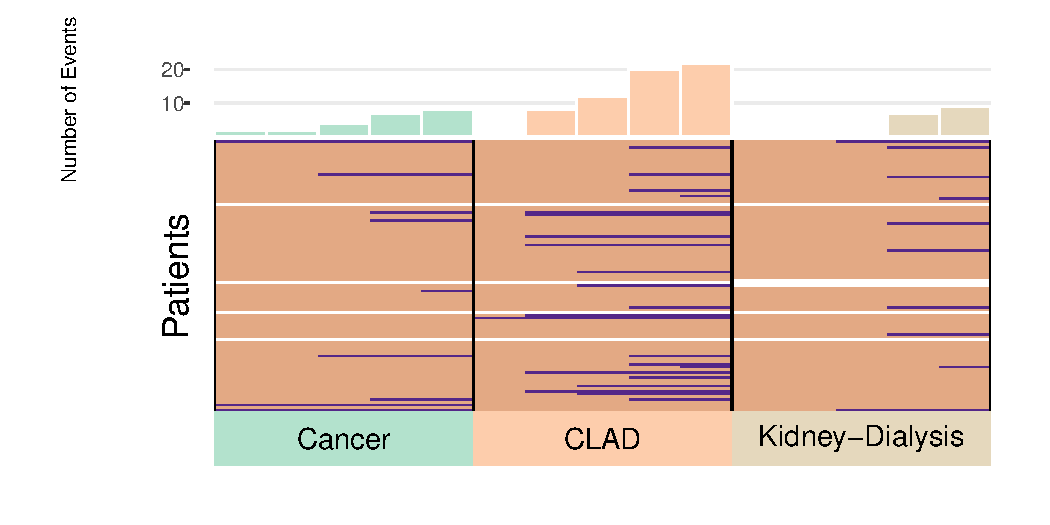
\includegraphics[width=\maxwidth]{plots/ptimedep_heatmap-1} 

\end{knitrout}
\caption{Time-dependent factors of the whole study population} \label{fig:fig5}
\end{figure}


Figure \ref{fig:fig5} shows the whole distribution of those three time-dependent factors among those 99 cystic fibrosis patients. The large orange part represents those patients who did not suffer from those three problems (Cancer, CLAD and Kidney Problems) during whole period of follow-up time. The corresponding proportion was very large, corresponding to the small number of events for any time period in table \ref{tab:tab2}.

Purple horizontal lines in figure \ref{fig:fig5} indicate those patients who got CLAD, Cancer or Kidney-Dialysis after lung transplantation. Similarly in the histogram above the heatmap, the number of patients has increased with time.

White horizontal lines showed there are some patients, whose information about \textit{Cancer}, \textit{CLAD} and \textit{Kidney-Dialysis} were missing. 

Number of missing values was illustrated in table \ref{tab:tab2}. We lost the information for all three events of 4 patients and additional 2 patients for \textit{Kidney-Dialysis}. 

From the bar on the top of this figure, \textit{CLAD} is much more common and \textit{Kidney-Dialysis} had the smallest number of events. Each bar illustrated the the number of events for each time point after transplantation. During the whole period of follow-up time, number of events for all those three diseases had increased with time. The number of events for all those three complication, rejection or transplantation-related disease were very small. In table \ref{tab:tab2}, the largest number of events was the number of patients for CLAD, 22 measured at the end of the study. 




\clearpage
% =======================================
\subsection*{Data Description for outcomes} \label{subsec:outcomes}
% =======================================
% =======================================
\subsubsection*{Data description for work percentage after LTx}\label{subsubsec:perc}
% =======================================




\begin{figure}[ht]
\centering
\begin{knitrout}
\definecolor{shadecolor}{rgb}{0.969, 0.969, 0.969}\color{fgcolor}
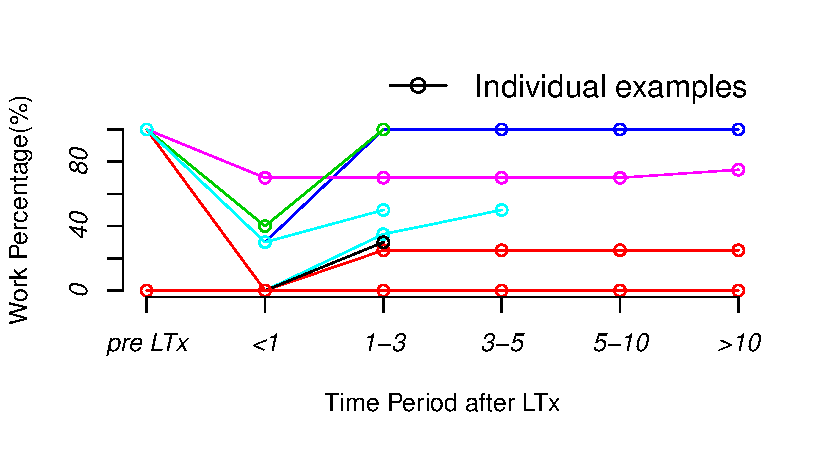
\includegraphics[width=\maxwidth]{plots/ptenperc-1} 

\end{knitrout}
\caption{Work percentage for 10 samples during different time periods} \label{fig:fig6}
\end{figure}

In figure \ref{fig:fig6}, we selected ten patients randomly, each line in the figure represents a single patient. It showed how did the work percentage at each time point change with time. The first time point "pre LTx" indicates the pre-transplantation work percentage, being estimated by the Pre-employed or Pre-not employed status. Therefore, the information of the pre-transplantation work percentage is not biased. We treated those non-employed before lung transplantation before as 0 for work percentage and those employed before lung transplantation as 100(\%) of work parentage. These estimates are not accurate, but it can help to show the change of work participation over time after lung transplantation.

It is natural that patients would work less or never work right after lung transplantation, to allow optimal healing. One year after lung transplantation, work percentage started to increase. Three years later, the work percentage of those 10 patients seems to be more or less stable. It should not been ignored that, there are more and more loss to follow-up with time, even though there are only ten patients as a sample there, we can also see that average of work percentage of some patients was not accessible for later period of time.
\clearpage




\begin{figure}[ht]
\centering
\begin{knitrout}
\definecolor{shadecolor}{rgb}{0.969, 0.969, 0.969}\color{fgcolor}
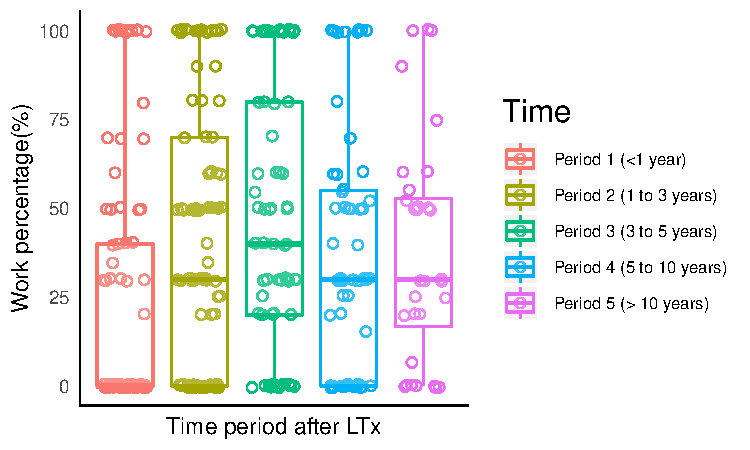
\includegraphics[width=\maxwidth]{plots/pworkperc-1} 

\end{knitrout}
\caption{Post-transplantation work percentage of all the periods}\label{fig:fig7}
\end{figure}


We used the estimated pre-transplantation work percentage and only showed the post-transplantation work percentage of a sample of patients with size 10 in figure \ref{fig:fig6}. Figure \ref{fig:fig7} showed the work percentage after transplantation of whole study population. The dots in colors indicate the work percentage of patient at each time point after transplantation. The box for each time point shows distribution of work percentage. The upper and lower "hinges" correspond to the first and third quantile, and the middle line indicate the mean of work percentage. From the left to the right, the later of the follow-up period of time, the more patients were loss to follow-up. From \ref{tab:tab3, the last period of time, \textit{Period 5} had only one thirds patients left.

Similar to what we have seen in figure \ref{fig:fig6} of 10 samples. Within one year after lung transplantation, there were many patients not working at all. It seems to be stable for the mean of work percentage during later time periods, although the information of a large number of patients were not accessible. 

Since there was a large proportion of patients not working at all within one year after lung transplantation, we would check the residuals for our final model.


\clearpage
% =======================================
\subsubsection*{Data description for work status after LTx}\label{subsubsec:status}
% =======================================
\begin{figure}[ht]
\centering
\begin{knitrout}
\definecolor{shadecolor}{rgb}{0.969, 0.969, 0.969}\color{fgcolor}
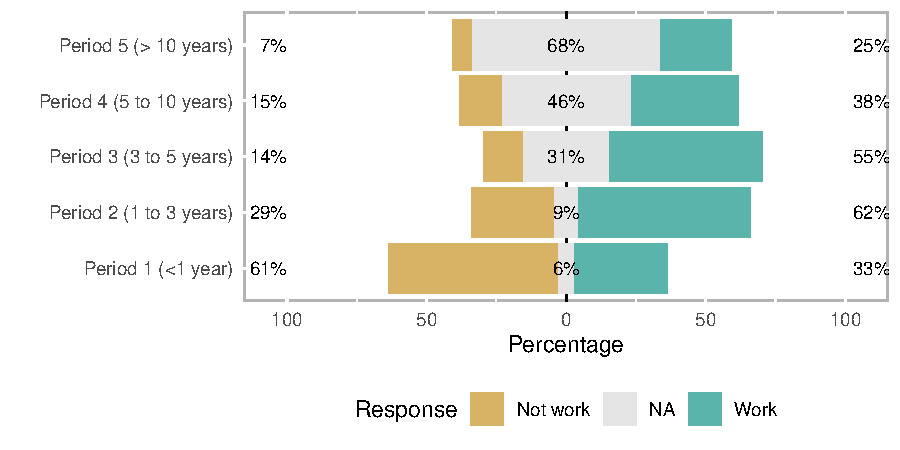
\includegraphics[width=\maxwidth]{plots/pworkstat-1} 

\end{knitrout}
\caption{Work status after LTx for all time periods}\label{fig:fig8}
\end{figure}


% latex table generated in R 3.5.2 by xtable 1.8-4 package
% Thu Oct 10 20:45:50 2019
\begin{table}[ht]
\centering
\caption{Post-LTx work status} 
\label{tab:tab3}
\scalebox{1}{
\begin{tabular}{rrrrrr}
  \hline
 & Period 1 & Period 2 & Period 3 & Period 4 & Period 5 \\ 
  \hline
Work &  60 &  29 &  14 &  15 &   7 \\ 
  Not work &  33 &  61 &  54 &  38 &  25 \\ 
  NA &   6 &   9 &  31 &  46 &  67 \\ 
  Total &  93 &  90 &  68 &  53 &  32 \\ 
   \hline
\end{tabular}
}
\end{table}


When it comes to work status after lung transplantation, figure \ref {fig:fig8} and table\ref{tab:tab3} showed that, the proportion of loss to follow-up has increased a lot during the follow-up time periods, from 6\% of the whole study population to 68\% of the whole study population. The proportion of  not working patients after transplantation decreased monotonously, from 61\% to 7\%.

\clearpage
% =======================================
\section{Results} \label{sec:results}
% =======================================
The first step was logistic regression for post-transplantation work status and linear regression for post-transplantation work percentage with respect to each time point after lung transplantation.

From table \ref{tab:tab2}, time-dependent factors \textit{CLAD}, \textit{Cancer} and \textit{Kidney-Dialysis} did not have enough number of events. Therefore, we did not take those three time-dependent factors into consideration before the analysis for repeated measurements.

We used BIC for model selection. 

% =======================================
\subsection*{Logistic regression for post-transplantation work status} \label{subsec:logis}
% =======================================
% =======================================
\subsubsection*{Post-transplantation work status within one year} \label{subsubsec:logis1}
% =======================================

%Variable Selection based on AUC and BIC


% latex table generated in R 3.5.2 by xtable 1.8-4 package
% Thu Oct 10 20:45:51 2019
\begin{table}[ht]
\centering
\caption{Univariate models for work status 
                within one year after LTx} 
\scalebox{0.8}{
\begin{tabular}{rrllrr}
  \hline
 & Odds Ratio & $95\%$-confidence interval & $p$-value & AUC & BIC \\ 
  \hline
Age & 0.98 & from 0.94 to 1.03 & 0.48 & 0.54 & 105.15 \\ 
  Best FEV1(\%) & 1.00 & from 0.97 to 1.02 & 0.81 & 0.59 & 104.97 \\ 
  BMI & 0.89 & from 0.75 to 1.03 & 0.14 & 0.59 & 102.81 \\ 
  Education(Academic) & 2.17 & from 0.79 to 6.02 & 0.13 & 0.57 & 103.40 \\ 
  Living(Alone) & 0.35 & from 0.08 to 1.20 & 0.12 & 0.57 & 102.56 \\ 
  Pre-employment(Employed) & 8.67 & from 3.33 to 25.12 & < 0.0001 & 0.74 & 88.84 \\ 
  Relationship(Single) & 1.42 & from 0.56 to 3.73 & 0.47 & 0.55 & 104.70 \\ 
  Sex(Male) & 0.99 & from 0.42 to 2.34 & 0.99 & 0.54 & 105.09 \\ 
  6MWD & 1.00 & from 0.99 to 1.00 & 0.43 & 0.56 & 104.57 \\ 
  Waiting time & 1.00 & from 0.99 to 1.01 & 0.94 & 0.58 & 104.93 \\ 
   \hline
\end{tabular}
}
\end{table}



AUC and BIC were calculated based on the same dataset, which removed patients with missing values. Odds ratios and corresponding 95\% confidence interval were calculated from the whole dataset. 

Within one year after lung transplantation, there are 60 patients did not work and 33 worked. Our selected model would have at most three predictors.

The univariate model with predictor \textit{Pre-employment}, has the much smaller BIC (88.84) than other univariate models. It may have much more strong effect on the post-transplantation work status than other factors. We would like to take it as a predictor in any of the selected models. 

% latex table generated in R 3.5.2 by xtable 1.8-4 package
% Thu Oct 10 20:45:51 2019
\begin{table}[ht]
\centering
\caption{Model selection for 
                   work status within one year after LTx} 
\label{tab:tab5}
\scalebox{0.8}{
\begin{tabular}{rr}
  \hline
 & BIC \\ 
  \hline
Pre-employment+Living+Education & 92.30 \\ 
  Pre-employment+Education & 91.96 \\ 
  Pre-employment+Living & 89.46 \\ 
  Pre-employment & 88.84 \\ 
   \hline
\end{tabular}
}
\end{table}



% latex table generated in R 3.5.2 by xtable 1.8-4 package
% Thu Oct 10 20:45:51 2019
\begin{table}[!h]
\centering
\caption{Selected model for work status 
                less than one year after LTx} 
\label{tab:tab6}
\begingroup\footnotesize
\begin{tabular}{rrrr}
  \hline
 & Odds Ratio & 95\%-confidence interval & $p$-value \\ 
  \hline
Pre-employment(Employed) & 8.67 & from 3.33 to 25.12 & $<$ 0.0001 \\ 
   \hline
\end{tabular}
\endgroup
\end{table}


Based on the the odds ratio from those univariate models, factors \textit{Education} and \textit{Living} also seem to have relatively strong effect on the post-transplantation work status. We compared the BIC values of all possible models, as is illustrated in table \ref{tab:tab5}.

With the smallest value of BIC (88.84), we determine \textit{Pre-employment} as the only  predictor for post-transplantation work status one year after lung transplantation. The result from table \ref{tab:tab6} shows that there is strong evidence for association between \textit{Pre-employment} and work status within one year after lung transplantation. \textit{Pre-employment} is the predictor we determined for work status within one year after lung transplantation.

\vspace*{1cm}

% =======================================
\subsubsection*{Post-transplantation work status one to three years} \label{subsubsec:logis2}
% =======================================

% latex table generated in R 3.5.2 by xtable 1.8-4 package
% Thu Oct 10 20:45:52 2019
\begin{table}[ht]
\centering
\caption{Univariate models for work status one to three years after LTx} 
\scalebox{0.8}{
\begin{tabular}{rrllrr}
  \hline
 & Odds Ratio & $95\%$-confidence interval & $p$-value & AUC & BIC \\ 
  \hline
Age & 0.95 & from 0.91 to 1.00 & 0.04 & 0.63 & 95.97 \\ 
  Best FEV1(\%) & 1.00 & from 0.98 to 1.03 & 0.92 & 0.62 & 98.92 \\ 
  BMI & 0.91 & from 0.78 to 1.05 & 0.21 & 0.45 & 97.37 \\ 
  Education(Academic) & 5.22 & from 1.35 to 34.53 & 0.04 & 0.62 & 92.92 \\ 
  Living(Alone) & 0.78 & from 0.26 to 2.54 & 0.67 & 0.51 & 99.53 \\ 
  Pre-employment(Employed) & 11.08 & from 3.73 to 41.39 & < 0.0001 & 0.80 & 72.59 \\ 
  Relationship(Single) & 1.61 & from 0.63 to 4.06 & 0.31 & 0.58 & 97.88 \\ 
  Sex(Male) & 0.51 & from 0.20 to 1.25 & 0.15 & 0.59 & 97.52 \\ 
  6MWD & 1.00 & from 1.00 to 1.00 & 1.00 & 0.54 & 99.52 \\ 
  Waiting time & 1.01 & from 1.00 to 1.03 & 0.13 & 0.55 & 98.21 \\ 
   \hline
\end{tabular}
}
\end{table}



Similarly, from the result of univariate models one to three years after lung transplantation, the one with \textit{Pre-employment} as the only predictor has much lower BIC than other univariate models. The number of patients work work after lung transplantation is 29. Therefore, we would also take at most 3 predictors into consideration.

The results of odds ratios of univariate models show that, besides \textit{Pre-employment}, model with \textit{Education} is the only one whose odds ratio is far from 1. Therefore, \textit{Education} and \textit{Pre-employment} are possible predictors for work status one to three years after lung transplantation.


% latex table generated in R 3.5.2 by xtable 1.8-4 package
% Thu Oct 10 20:45:52 2019
\begin{table}[ht]
\centering
\caption{Model selection for work status one to three years after LTx} 
\scalebox{0.8}{
\begin{tabular}{rr}
  \hline
 & BIC \\ 
  \hline
Pre-employment & 72.59 \\ 
  Pre-employment+Education & 70.33 \\ 
   \hline
\end{tabular}
}
\end{table}



The results determined \textit{Pre-employment} and \textit{Education} both as the predictors for work status one to three years after lung transplantation.

% latex table generated in R 3.5.2 by xtable 1.8-4 package
% Thu Oct 10 20:45:52 2019
\begin{table}[!h]
\centering
\caption{Selected model for work status one to three years after LTx} 
\label{tab:tab9}
\begingroup\footnotesize
\begin{tabular}{rrrr}
  \hline
 & Odds Ratio & 95\%-confidence interval & $p$-value \\ 
  \hline
Pre-employment(Employed) & 11.19 & from 3.67 to 42.71 & $<$ 0.0001 \\ 
  Education(Academic) & 5.34 & from 1.22 to 37.82 & 0.045 \\ 
   \hline
\end{tabular}
\endgroup
\end{table}


Table \ref{tab:tab9} shows there is also strong evidence that \textit{Pre-employment} has an effect on the work status. The evidence for \textit{Education} as a predictor is moderate.  

\clearpage
% =======================================
\subsubsection*{Post-transplantation work status three to five years} \label{subsubsec:logis3}
% =======================================

\begin{figure}[ht]
\begin{knitrout}
\definecolor{shadecolor}{rgb}{0.969, 0.969, 0.969}\color{fgcolor}
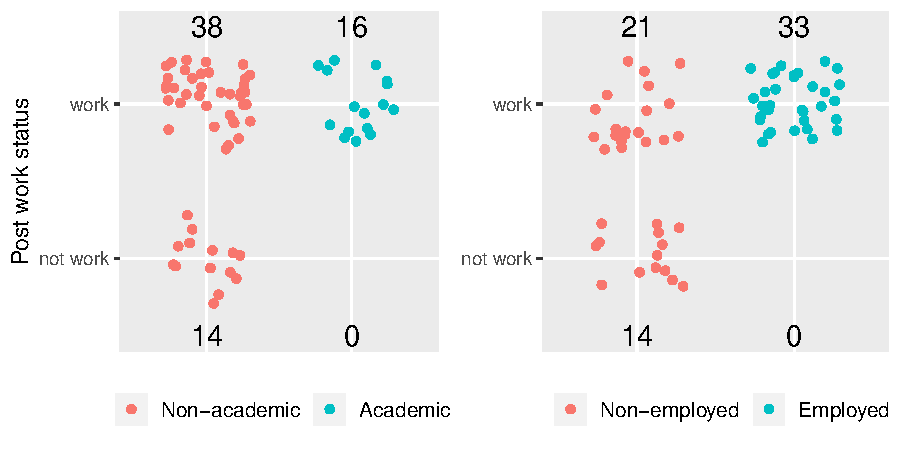
\includegraphics[width=\maxwidth]{plots/ptwoby2plot-1} 

\end{knitrout}
\caption{Work status with respect to Pre-employment and Education for three to five year after LTx}\label{fig9}
\end{figure}


There are some extreme cases as shown in figure \ref{fig9}. We could not analysis the association between \textit{Education} and \textit{Pre-employment},
no academic-educated or pre-employed not working three to five years after transplantation.

It shows association between those two factors, \textit{Education} and \textit{Pre-employment} and the post-transplantation work status during this time period.

From the univariate models in \ref{tab:tab10}, it is clear that, in spite of \textit{Education} and \textit{Pre-employment}, odds ratio for any of those factor are not far from 1, indicating not very strong effect on the work status.

Since we would do further analyses, we do not choose any kind of correction ways to do regress for work status for those time periods.

% latex table generated in R 3.5.2 by xtable 1.8-4 package
% Thu Oct 10 20:45:53 2019
\begin{table}[ht]
\centering
\caption{Univariate models for work status three to five years after LTx} 
\label{tab:tab10}
\scalebox{0.8}{
\begin{tabular}{rrllrr}
  \hline
 & Odds Ratio & $95\%$-confidence interval & $p$-value & AUC & BIC \\ 
  \hline
Age & 0.96 & from 0.91 to 1.02 & 0.16 & 0.66 & 60.28 \\ 
  Best FEV1(\%) & 0.98 & from 0.95 to 1.02 & 0.41 & 0.67 & 62.74 \\ 
  BMI & 0.95 & from 0.80 to 1.16 & 0.60 & 0.63 & 63.22 \\ 
  Living(Alone) & 0.39 & from 0.10 to 1.71 & 0.19 & 0.58 & 63.98 \\ 
  Relationship(Single) & 1.05 & from 0.29 to 3.53 & 0.94 & 0.59 & 64.54 \\ 
  Sex(Male) & 0.87 & from 0.26 to 2.84 & 0.82 & 0.57 & 64.64 \\ 
  6MWD & 1.00 & from 0.99 to 1.00 & 0.75 & 0.44 & 64.61 \\ 
  Waiting time & 1.00 & from 0.99 to 1.02 & 0.80 & 0.55 & 64.62 \\ 
   \hline
\end{tabular}
}
\end{table}



\clearpage

% =======================================
\subsubsection*{Post-transplantation work status five to ten years} \label{subsubsec:logis4}
% =======================================
% latex table generated in R 3.5.2 by xtable 1.8-4 package
% Thu Oct 10 20:45:54 2019
\begin{table}[ht]
\centering
\caption{Univariate models for work status five to ten years after LTx} 
\scalebox{0.8}{
\begin{tabular}{rrllrr}
  \hline
 & Odds Ratio & $95\%$-confidence interval & $p$-value & AUC & BIC \\ 
  \hline
Age & 0.94 & from 0.88 to 1.00 & 0.07 & 0.64 & 57.33 \\ 
  Best FEV1(\%) & 0.98 & from 0.94 to 1.02 & 0.34 & 0.64 & 58.91 \\ 
  BMI & 0.90 & from 0.71 to 1.11 & 0.33 & 0.51 & 58.65 \\ 
  Education(Academic) & 6.46 & from 1.09 to 123.87 & 0.09 & 0.64 & 54.93 \\ 
  Living(Alone) & 0.44 & from 0.10 to 2.07 & 0.28 & 0.57 & 58.22 \\ 
  Pre-employment(Employed) & 26.92 & from 4.64 to 515.70 & 0.0025 & 0.79 & 44.87 \\ 
  Relationship(Single) & 1.00 & from 0.26 to 3.52 & 1.00 & 0.55 & 58.78 \\ 
  Sex(Male) & 0.88 & from 0.26 to 2.91 & 0.83 & 0.54 & 58.96 \\ 
  6MWD & 1.00 & from 0.99 to 1.00 & 0.47 & 0.45 & 58.85 \\ 
  Waiting time & 1.00 & from 0.98 to 1.03 & 0.85 & 0.53 & 58.93 \\ 
   \hline
\end{tabular}
}
\end{table}




% latex table generated in R 3.5.2 by xtable 1.8-4 package
% Thu Oct 10 20:45:54 2019
\begin{table}[ht]
\centering
\caption{Model selection for 
                   work status five to ten years after LTx} 
\label{tab:tab11}
\scalebox{0.8}{
\begin{tabular}{rr}
  \hline
 & BIC \\ 
  \hline
Pre-employment & 44.87 \\ 
  Pre-employment+Education & 41.71 \\ 
   \hline
\end{tabular}
}
\end{table}



% latex table generated in R 3.5.2 by xtable 1.8-4 package
% Thu Oct 10 20:45:54 2019
\begin{table}[!h]
\centering
\caption{Selected model for work status 
                five to ten years after LTx} 
\label{tab:tab12}
\begingroup\footnotesize
\begin{tabular}{rrrr}
  \hline
 & Odds Ratio & 95\%-confidence interval & $p$-value \\ 
  \hline
Pre-employment(Employed) & 36.51 & from 5.84 to 724.49 & 0.001 \\ 
  Education(Academic) & 11.56 & from 1.61 to 240.46 & 0.036 \\ 
   \hline
\end{tabular}
\endgroup
\end{table}




For time period three to five years after lung transplantation, there are 15 patients did not work and 38 worked.
We took at most 2 predictors into consideration for selected model. It is very obvious that \textit{Education} and \textit{Pre-employment} are the two possible predictors for selected model, as the univariate models for those two show much more strong effect on post-transplantation work status than other factors.

From table \ref{tab:tab11} and \ref{tab:tab12}, we determine \textit{Pre-employment} and \textit{Education} as the predictors for the work status five to ten years after lung transplantation. The evidence for those two predictors are strong for \textit{Pre-employment} and moderate for \textit{Education}.

\clearpage
% =======================================
\subsubsection*{Post-transplantation work status longer than ten years} \label{subsubsec:logis3}
% =======================================
\begin{figure}[ht]
\begin{knitrout}
\definecolor{shadecolor}{rgb}{0.969, 0.969, 0.969}\color{fgcolor}
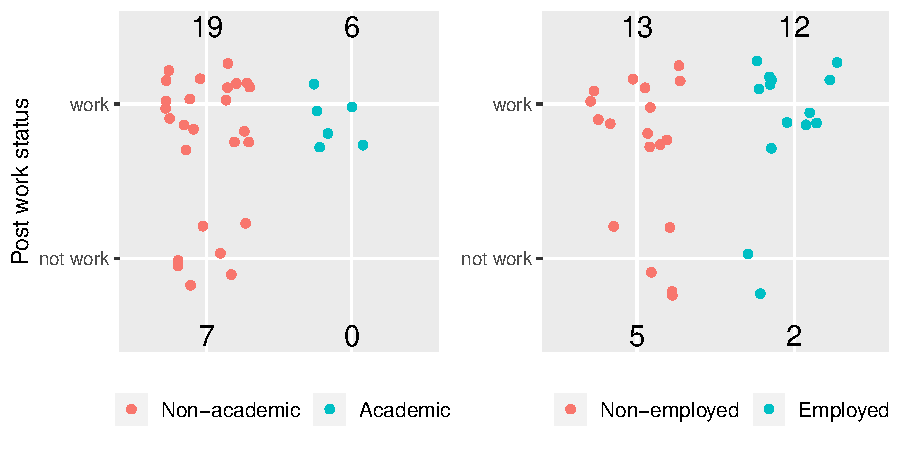
\includegraphics[width=\maxwidth]{plots/ptwoby2plot2-1} 

\end{knitrout}
\caption{Work status with respect to Pre-employment and Education for longer than ten years after LTx}\label{fig10}
\end{figure}


% latex table generated in R 3.5.2 by xtable 1.8-4 package
% Thu Oct 10 20:45:55 2019
\begin{table}[ht]
\centering
\caption{Univariate models for work status
                 longer than ten years after LTx} 
\label{tab:tabadd}
\scalebox{0.8}{
\begin{tabular}{rrllrr}
  \hline
 & Odds Ratio & $95\%$-confidence interval & $p$-value & AUC & BIC \\ 
  \hline
Age & 0.92 & from 0.82 to 1.01 & 0.11 & 0.66 & 32.74 \\ 
  Best FEV1(\%) & 0.98 & from 0.93 to 1.03 & 0.47 & 0.67 & 34.31 \\ 
  BMI & 0.78 & from 0.51 to 1.00 & 0.13 & 0.63 & 32.16 \\ 
  Living(Alone) & 0.24 & from 0.02 to 2.37 & 0.20 & 0.58 & 33.72 \\ 
  Relationship(Single) & 2.70 & from 0.42 to 16.86 & 0.28 & 0.59 & 33.83 \\ 
  Sex(Male) & 1.23 & from 0.23 to 7.35 & 0.81 & 0.57 & 34.19 \\ 
  6MWD & 1.00 & from 0.99 to 1.01 & 0.48 & 0.44 & 34.27 \\ 
  Waiting time & 1.00 & from 0.96 to 1.06 & 0.88 & 0.55 & 34.50 \\ 
   \hline
\end{tabular}
}
\end{table}


Similarly to the time period three to five years after lung transplantation, In figure \ref{fig10}, there were few cases for academic-educated and pre-employed patients not working after transplantation. 

We did not analyse the association between \textit{Education}, \textit{Pre-employment} and work status after transplantation. 

From the univariate models in \ref{tab:tabadd}, it is clear that, those factors, in spite of \textit{Education} and \textit{Pre-employment}, do not have very strong effect on the outcome.


\clearpage

% =======================================
\subsubsection*{Post-transplantation work status for all time periods} \label{subsubsec:logis_all}

% latex table generated in R 3.5.2 by xtable 1.8-4 package
% Thu Oct 10 20:45:55 2019
\begin{table}[ht]
\centering
\caption{Result for logistic regression 
                  for all possible periods after LTx} 
\label{tab:tab13}
\scalebox{0.8}{
\begin{tabular}{rlll}
  \hline
 & Odds Ratio & $95\%$-confidence interval & $p$-value \\ 
  \hline
Pre-employment(<1) & 8.67 & from 3.33 to 25.12 & < 0.0001 \\ 
  Pre-employment(1-3) & 11.19 & from 3.67 to 42.71 & < 0.0001 \\ 
  Pre-employment(5-10) & 36.51 & from 5.84 to 724.49 & 0.001 \\ 
   & - & - & - \\ 
  Education(3-5) & 5.34 & from 1.22 to 37.82 & 0.045 \\ 
  Education(5-10) & 11.56 & from 1.61 to 240.46 & 0.036 \\ 
   \hline
\end{tabular}
}
\end{table}



Table \ref{tab:tab13} showed all of the results of logistic regression for three time periods, within one year, one to three year and five to ten years after transplantation. 

There are two possible predictors for post-transplantation work status. \textit{Pre-employment} is the dominant one with very strong or strong of evidence. \textit{Education} is another predictor with moderate evidence for association with the work status after lung transplantation. 

The width of 95\% confidence intervals for both predictors increased with time, due to more and more loss to follow-up with time. 


\clearpage
% =======================================
\subsection*{Linear regression for post-transplantation work percentage} \label{subsec:linear}
% =======================================
\vspace*{0.5cm}
% =======================================
\subsubsection*{Post-transplantation work percentage within one year} \label{subsubsection:linear1}
% =======================================




% latex table generated in R 3.5.2 by xtable 1.8-4 package
% Thu Oct 10 20:45:56 2019
\begin{table}[ht]
\centering
\caption{Univariate models for work percentage 
                  less than one year after LTx} 
\label{tab:tab14}
\scalebox{0.8}{
\begin{tabular}{rrllr}
  \hline
 & Coefficient & $95\%$-confidence interval & $p$-value & BIC \\ 
  \hline
Age & -0.78 & from -1.46 to -0.09 & 0.04 & 742.15 \\ 
  Best FEV1(\%) & -0.20 & from -0.59 to 0.20 & 0.11 & 743.70 \\ 
  BMI & -2.23 & from -4.46 to 0.00 & 0.08 & 743.10 \\ 
  Education(Academic) & 2.20 & from -15.02 to 19.42 & 0.94 & 746.35 \\ 
  Living(Alone) & -16.98 & from -34.32 to 0.37 & 0.09 & 743.35 \\ 
  Pre-employment(Employed) & 30.71 & from 18.06 to 43.36 & < 0.0001 & 728.85 \\ 
  Relationship(Single) & 14.36 & from 0.11 to 28.61 & 0.05 & 742.32 \\ 
  Sex(Male) & -0.87 & from -15.03 to 13.29 & 0.49 & 745.86 \\ 
  6MWD & -0.03 & from -0.10 to 0.04 & 0.30 & 745.26 \\ 
  Waiting time & -0.06 & from -0.24 to 0.13 & 0.22 & 744.78 \\ 
   \hline
\end{tabular}
}
\end{table}



% latex table generated in R 3.5.2 by xtable 1.8-4 package
% Thu Oct 10 20:45:56 2019
\begin{table}[ht]
\centering
\caption{Model selection for 
               work percentage less than one year after LTx} 
\label{tab:tab15}
\scalebox{0.8}{
\begin{tabular}{rr}
  \hline
 & BIC \\ 
  \hline
Pre-employment+Living+Education & 733.38 \\ 
  Pre-employment+Education & 732.99 \\ 
  Pre-employment+Living & 729.21 \\ 
  Pre-employment & 728.85 \\ 
   \hline
\end{tabular}
}
\end{table}



% latex table generated in R 3.5.2 by xtable 1.8-4 package
% Thu Oct 10 20:45:56 2019
\begin{table}[!h]
\centering
\caption{Selected model for work percentage
                one to three years after LTx} 
\begingroup\footnotesize
\begin{tabular}{rrrr}
  \hline
 & Coefficient & 95\%-confidence interval & $p$-value \\ 
  \hline
Pre-employment(Employed) & 30.71 & from 18.06 to 43.36 & $<$ 0.0001 \\ 
   \hline
\end{tabular}
\endgroup
\end{table}


For those univariate models for linear regression for work percentage, we choose \textit{Pre-employment}, \textit{Living}, \textit{Education} for model selection, since those three seem to have much more strong effect on the outcome than the others from the coefficients from table \ref{tab:tab14}.

After model selection based on BIC, we determined \textit{pre-employment} as the predictor for work percentage one year after lung transplantation. Form the $p$-value in the table \ref{tab:tab15}, we can also see strong evidence for this predictor.

\clearpage
% =======================================
\subsubsection*{Post-transplantation work percentage one to three years} \label{subsubsection:linear2}
% =======================================
% latex table generated in R 3.5.2 by xtable 1.8-4 package
% Thu Oct 10 20:45:56 2019
\begin{table}[ht]
\centering
\caption{Univariate models for work percentage 
                  one to three years after LTx} 
\scalebox{0.8}{
\begin{tabular}{rrllr}
  \hline
 & Coefficient & $95\%$-confidence interval & $p$-value & BIC \\ 
  \hline
Age & -1.20 & from -1.91 to -0.48 & 0.0013 & 732.13 \\ 
  Best FEV1(\%) & 0.00 & from -0.44 to 0.45 & 0.99 & 740.81 \\ 
  BMI & -3.40 & from -5.85 to -0.94 & 0.0072 & 735.00 \\ 
  Education(Academic) & 15.73 & from -3.11 to 34.56 & 0.10 & 740.01 \\ 
  Living(Alone) & -20.07 & from -39.89 to -0.25 & 0.05 & 738.99 \\ 
  Pre-employment(Employed) & 35.41 & from 21.69 to 49.12 & < 0.0001 & 714.92 \\ 
  Relationship(Single) & 13.66 & from -2.58 to 29.90 & 0.10 & 737.90 \\ 
  Sex(Male) & -6.16 & from -21.79 to 9.46 & 0.44 & 740.38 \\ 
  6MWD & -0.00 & from -0.08 to 0.07 & 0.94 & 741.17 \\ 
  Waiting time & 0.13 & from -0.07 to 0.32 & 0.20 & 740.02 \\ 
   \hline
\end{tabular}
}
\end{table}



% latex table generated in R 3.5.2 by xtable 1.8-4 package
% Thu Oct 10 20:45:56 2019
\begin{table}[ht]
\centering
\caption{Model selection for work percentage 
               one to three years after LTx} 
\scalebox{0.8}{
\begin{tabular}{rr}
  \hline
 & BIC \\ 
  \hline
Pre-employment+Education & 718.51 \\ 
  Pre-employment+Living+Education & 718.44 \\ 
  Pre-employment+Living & 715.06 \\ 
  Pre-employment & 714.92 \\ 
   \hline
\end{tabular}
}
\end{table}



% latex table generated in R 3.5.2 by xtable 1.8-4 package
% Thu Oct 10 20:45:56 2019
\begin{table}[!h]
\centering
\caption{Selected model for work percentage one to three years after LTx} 
\label{tab:tab19}
\begingroup\footnotesize
\begin{tabular}{rrrr}
  \hline
 & Coefficient & 95\%-confidence interval & $p$-value \\ 
  \hline
Pre-employment(Employed) & 35.41 & from 21.69 to 49.12 & $<$ 0.0001 \\ 
   \hline
\end{tabular}
\endgroup
\end{table}


The possible predictors for work percentage one to three years after lung transplantation, are \textit{Pre-employment}, \textit{Living} and \textit{Education.} Although the model with \textit{Pre-employment} and \textit{Education} as the predictors have the smallest BIC, we would also choose the model with only \textit{Pre-employment} as the predictor. Since the difference between these two model is smaller than 2, and we would like to choose the one with smaller number of predictors.

$P$-value in table \ref{tab:tab19} also showed strong evidence for \textit{Pre-employment} as a predictor, but the 95\% confidence interval is wider than before due to smaller sample size.

\clearpage
% =======================================
\subsubsection*{Post-transplantation work percentage three to five years} \label{subsubsection:linear3}
% =======================================
% latex table generated in R 3.5.2 by xtable 1.8-4 package
% Thu Oct 10 20:45:56 2019
\begin{table}[ht]
\centering
\caption{Univariate models for work percentage 
                  three to five years after LTx} 
\scalebox{0.8}{
\begin{tabular}{rllll}
  \hline
 & Coefficient & $95\%$-confidence interval & $p$-value & BIC \\ 
  \hline
Age & -1.27 & from -2.05 to -0.49 & 0.0019 & 528.53 \\ 
  Best FEV1(\%) & -0.30 & from -0.82 to 0.22 & 0.26 & 534.18 \\ 
  BMI & -3.46 & from -6.25 to -0.66 & 0.02 & 531.87 \\ 
  Education(Academic) & 20.00 & from -0.38 to 40.38 & 0.05 & 536.27 \\ 
  Living(Alone) & -20.91 & from -44.13 to 2.31 & 0.08 & 536.50 \\ 
  Pre-employment(Employed) & 38.69 & from 23.66 to 53.73 & < 0.0001 & 514.05 \\ 
  Relationship(Single) & 13.28 & from -5.04 to 31.59 & 0.15 & 536.42 \\ 
  Sex(Male) & -3.65 & from -21.48 to 14.18 & 0.68 & 538.32 \\ 
  6MWD & -0.01 & from -0.10 to 0.07 & 0.77 & 538.25 \\ 
  Waiting time & 0.13 & from -0.12 to 0.39 & 0.31 & 537.75 \\ 
   \hline
\end{tabular}
}
\end{table}


% latex table generated in R 3.5.2 by xtable 1.8-4 package
% Thu Oct 10 20:45:56 2019
\begin{table}[ht]
\centering
\caption{Model selection for work percentage three to five years after LTx} 
\scalebox{0.8}{
\begin{tabular}{rr}
  \hline
 & BIC \\ 
  \hline
Pre-employment+Living+Education & 515.77 \\ 
  Pre-employment+Education & 515.60 \\ 
  Pre-employment+Living & 515.12 \\ 
  Pre-employment & 514.05 \\ 
   \hline
\end{tabular}
}
\end{table}


% latex table generated in R 3.5.2 by xtable 1.8-4 package
% Thu Oct 10 20:45:56 2019
\begin{table}[!h]
\centering
\caption{Selected model for work status three to five years after LTx} 
\begingroup\footnotesize
\begin{tabular}{rrrr}
  \hline
 & Coefficient & 95\%-confidence interval & $p$-value \\ 
  \hline
Pre-employment(Employed) & 38.69 & from 23.66 to 53.73 & $<$ 0.0001 \\ 
   \hline
\end{tabular}
\endgroup
\end{table}


For work percentage three to five years after lung transplantation, model with only \textit{Pre-employment} has the lowest BIC. The evidence for the association between \textit{Pre-employment} and work percentage is very strong during this time period. 

\clearpage
% =======================================
\subsubsection*{Post-transplantation work percentage five to ten years} \label{subsubsection:linear4}
% =======================================

% latex table generated in R 3.5.2 by xtable 1.8-4 package
% Thu Oct 10 20:45:56 2019
\begin{table}[ht]
\centering
\caption{Univariate models for work percentage 
                  five to ten years after LTx} 
\scalebox{0.8}{
\begin{tabular}{rrlll}
  \hline
 & Coefficient & $95\%$-confidence interval & $p$-value & BIC \\ 
  \hline
Age & -0.96 & from -1.89 to -0.03 & 0.04 & 394.83 \\ 
  Best FEV1(\%) & -0.20 & from -0.78 to 0.37 & 0.48 & 396.56 \\ 
  BMI & -2.31 & from -5.58 to 0.95 & 0.16 & 396.01 \\ 
  Education(Academic) & 20.38 & from -0.92 to 41.69 & 0.06 & 395.24 \\ 
  Living(Alone) & -24.89 & from -48.01 to -1.76 & 0.04 & 393.15 \\ 
  Pre-employment(Employed) & 32.92 & from 16.34 to 49.50 & 0.00021 & 379.69 \\ 
  Relationship(Single) & 4.62 & from -14.91 to 24.15 & 0.64 & 396.86 \\ 
  Sex(Male) & -7.63 & from -26.49 to 11.24 & 0.42 & 396.7 \\ 
  6MWD & -0.04 & from -0.12 to 0.05 & 0.41 & 395.98 \\ 
  Waiting time & 0.08 & from -0.25 to 0.40 & 0.64 & 396.83 \\ 
   \hline
\end{tabular}
}
\end{table}



% latex table generated in R 3.5.2 by xtable 1.8-4 package
% Thu Oct 10 20:45:57 2019
\begin{table}[ht]
\centering
\caption{Model selection for work percentage 
               five to ten years after LTx} 
\scalebox{0.8}{
\begin{tabular}{rr}
  \hline
 & BIC \\ 
  \hline
Pre-employment+Living+Education & 378.99 \\ 
  Pre-employment+Education & 379.85 \\ 
  Pre-employment & 379.69 \\ 
  Pre-employment+Living & 379.20 \\ 
   \hline
\end{tabular}
}
\end{table}



% latex table generated in R 3.5.2 by xtable 1.8-4 package
% Thu Oct 10 20:45:57 2019
\begin{table}[!h]
\centering
\caption{Selected model for work status five to ten years after LTx} 
\begingroup\footnotesize
\begin{tabular}{rrrr}
  \hline
 & Coefficient & 95\%-confidence interval & $p$-value \\ 
  \hline
Pre-employment(Employed) & 32.92 & from 16.34 to 49.50 & 0.0002 \\ 
   \hline
\end{tabular}
\endgroup
\end{table}


For work percentage five to ten years after lung transplantation, model with predictors, \textit{Pre-employment} and \textit{Living}, has the lowest BIC, but the BIC for model with only \textit{Pre-employment} as the predictor, is not so much larger than this one. Therefore, the predictor we determined is \textit{Pre-employment}.

\clearpage

% =======================================
\subsubsection*{Post-transplantation work percentage longer than ten year} \label{subsubsection:linear5}
% =======================================



% latex table generated in R 3.5.2 by xtable 1.8-4 package
% Thu Oct 10 20:45:57 2019
\begin{table}[ht]
\centering
\caption{Univariate models for work percentage longer than ten years after LTx} 
\scalebox{0.8}{
\begin{tabular}{rrlll}
  \hline
 & Coefficient & $95\%$-confidence interval & $p$-value & BIC \\ 
  \hline
Age & -1.01 & from -2.24 to 0.22 & 0.10 & 234.5 \\ 
  Best FEV1(\%) & -0.04 & from -0.72 to 0.64 & 0.90 & 236 \\ 
  BMI & -2.65 & from -5.75 to 0.45 & 0.09 & 234.38 \\ 
  Education(Academic) & 29.04 & from 1.58 to 56.50 & 0.04 & 233.62 \\ 
  Living(Alone) & -28.62 & from -62.83 to 5.60 & 0.10 & 233.41 \\ 
  Pre-employment(Employed) & 20.23 & from -1.74 to 42.20 & 0.07 & 229.41 \\ 
  Relationship(Single) & 8.25 & from -19.21 to 35.71 & 0.54 & 235.81 \\ 
  Sex(Male) & 2.00 & from -21.08 to 25.07 & 0.86 & 236.03 \\ 
  6MWD & -0.02 & from -0.16 to 0.12 & 0.74 & 235.84 \\ 
  Waiting time & 0.23 & from -0.36 to 0.81 & 0.44 & 235.57 \\ 
   \hline
\end{tabular}
}
\end{table}



% latex table generated in R 3.5.2 by xtable 1.8-4 package
% Thu Oct 10 20:45:57 2019
\begin{table}[ht]
\centering
\caption{Model selection for work percentage longer than ten years after LTx} 
\scalebox{0.8}{
\begin{tabular}{rr}
  \hline
 & BIC \\ 
  \hline
Pre-employment+Living & 231.79 \\ 
  Pre-employment+Living+Education & 231.47 \\ 
  Pre-employment & 229.41 \\ 
  Pre-employment+Education & 229.36 \\ 
   \hline
\end{tabular}
}
\end{table}



% latex table generated in R 3.5.2 by xtable 1.8-4 package
% Thu Oct 10 20:45:57 2019
\begin{table}[!h]
\centering
\caption{Selected model for work status longer than ten years after LTx} 
\begingroup\footnotesize
\begin{tabular}{rrrr}
  \hline
 & Coefficient & 95\%-confidence interval & $p$-value \\ 
  \hline
Pre-employment(Employed) & 20.23 & from -1.74 to 42.20 & 0.07 \\ 
   \hline
\end{tabular}
\endgroup
\end{table}


Though the model with lowest value of BIC is the one with \textit{Pre-employment} and \textit{Education}, we would still determine \textit{Pre-employment} as the only predictor. The difference between values of BIC of the those two models is smaller than two, so we choose the one with smaller number of predictors.

For this time period, we get the same result as the previous time periods, \textit{Pre-employment} is the predictor that we determined.

\clearpage
% =======================================
\subsubsection*{Post-transplantation work percentage for all time periods} \label{subsubsection:linear5}




% latex table generated in R 3.5.2 by xtable 1.8-4 package
% Thu Oct 10 20:45:57 2019
\begin{table}[ht]
\centering
\caption{Result for linear regression  for periods after LTx} 
\label{tab:tab29}
\scalebox{0.8}{
\begin{tabular}{rlll}
  \hline
 & Coefficients & $95\%$-confidence interval & $p$-value \\ 
  \hline
Pre-employment(<1) & 30.71 & from 18.06 to 43.36 & < 0.0001 \\ 
  Pre-employment(1-3) & 35.41 & from 21.69 to 49.12 & < 0.0001 \\ 
  Pre-employment(3-5) & 38.69 & from 23.66 to 53.73 & < 0.0001 \\ 
  Pre-employment(5-10) & 32.92 & from 16.34 to 49.50 & 0.0002 \\ 
  Pre-employment(>10) & 20.23 & from -1.74 to 42.20 & 0.07 \\ 
   \hline
\end{tabular}
}
\end{table}


From table \ref{tab:tab29}, we get the conclusion that, results for work percentage for all time periods are consistent. \textit{Pre-employment} is the only predictor that we determined for work percentage after lung transplantation. The evidence is very strong for the fist three time periods and relatively weaker for the last time period. 95\% confidence interval also gets wider and wider.



\clearpage
% =======================================
\subsection*{Longitudinal data analysis for post-transplantation work status} \label{subsec:LDA}
% =======================================
The aim of our study is to evaluate the long-term work participation after lung transplantation. In an attempt to take time, time-varying variables and repeated measurements of outcomes into one model, we did the longitudinal data analysis.

\begin{figure}[ht]
\centering
\begin{knitrout}
\definecolor{shadecolor}{rgb}{0.969, 0.969, 0.969}\color{fgcolor}
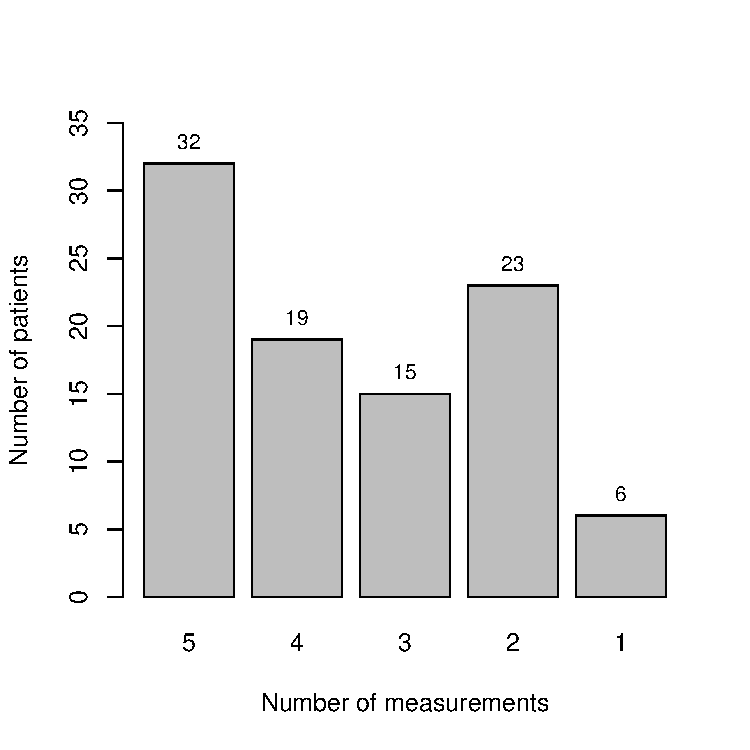
\includegraphics[width=\maxwidth]{plots/pnumber_measurements-1} 

\end{knitrout}
\caption{The number of patients corresponding to number of measurements}\label{fig:fig13}
\end{figure}
 
From figure \ref{fig:fig13}, we can see the number of repeated measurements are different for different patients. Since the time they got the lung transplantation are different, the study period for each patient are different. There are 32 patients, undergoing lung transplantation very early and have measurements for all five time points. 6 patients got the lung transplantation too late, we only had access to their measurements of work participation and the possible post-transplantation rejections and complications at the end of the study.

Based on those repeated measurements and the exact time for each patient, we got the long-format data. From the results from the previous results from linear regression and logistic regression for separate time points, we would be able to construct mixed-effects models for work status and work percentage after lung transplantation.


% =======================================
\subsubsection*{Generalized linear mixed effect model for work status after LTx}\label{subsubsec:GLMM}
% =======================================
From the results of logistic model, there are two possible predictors for the work  status after lung transplantation, \textit{Pre-employment} and \textit{Education}. We select model for longitudinal data analysis based on the result and three transformation of Time.

There a great number of ways to transform time, we chose the most common ones, log(Time), Time and $\mathrm{Time}^2$ , we selected the form of transformation with the lowest BIC.




% latex table generated in R 3.5.2 by xtable 1.8-4 package
% Thu Oct 10 20:45:57 2019
\begin{table}[ht]
\centering
\caption{Time transformation for work status after LTx based on BIC} 
\label{tab:tab30}
\begin{tabular}{rrr}
  \hline
 & Pre-employment & Education + Pre-employment \\ 
  \hline
log(Time) & 352.37 & 343.07 \\ 
  Time & 371.11 & 361.61 \\ 
  $(\mathrm{Time})^2$ & 383.84 & 373.83 \\ 
   \hline
\end{tabular}
\end{table}


Table \ref{tab:tab30} shows that we would choose log(Time) as the transformation for time. Both of the time-independent factors, \textit{Pre-employment} and \textit{Education} would go into our model for generalized linear mixed-effects model. 

% latex table generated in R 3.5.2 by xtable 1.8-4 package
% Thu Oct 10 20:45:57 2019
\begin{table}[ht]
\centering
\caption{Model selection for work status based on Time-dependent factors} 
\scalebox{0.8}{
\begin{tabular}{rrrrr}
  \hline
 & CLAD & Cancer & Kidney-Dialysis & BIC \\ 
  \hline
Model 1 & 0 & 0 & 1 & 333.75 \\ 
  Model 2 & 0 & 1 & 0 & 336.48 \\ 
  Model 3 & 1 & 0 & 0 & 337.00 \\ 
  Model 4 & 0 & 1 & 1 & 339.00 \\ 
  Model 5 & 1 & 0 & 1 & 339.48 \\ 
  Model 6 & 1 & 1 & 0 & 342.18 \\ 
  Model 7 & 1 & 1 & 1 & 344.69 \\ 
   \hline
\end{tabular}
}
\end{table}



From table \ref{tab:tab32}, among all those three time-dependent factors, we chose \textit{CLAD} as the only predictor for our model, and Time variable is transformed into as log(Time).




% latex table generated in R 3.5.2 by xtable 1.8-4 package
% Thu Oct 10 20:47:06 2019
\begin{table}[ht]
\centering
\caption{Result for Generalized Linear Mixed-effects Model 
for Post-LTx Work Status} 
\label{tab:tab32}
\scalebox{0.8}{
\begin{tabular}{rrll}
  \hline
 & Odds Ratio & $95\%$-confidence interval & $p$-value \\ 
  \hline
Pre-employment & 32.16 & from 9.48 to 177.09 & < 0.0001 \\ 
  Education & 4.40 & from 1.07 to 20.55 & 0.04 \\ 
  CLAD & 0.64 & from 0.15 to 2.40 & 0.49 \\ 
  log(Time) & 4.94 & from 2.95 to 9.38 & < 0.0001 \\ 
   \hline
\end{tabular}
}
\end{table}



The result from generalized linear fixed effect model \ref{tab:tab32} showed that there is moderate evidence that time-dependent factor, \textit{CLAD}, is the predictor for post-transplantation work status.  



\clearpage
% =======================================
\subsubsection*{Linear mixed-effect model for work status after LTx}\label{subsubsec:LMM}
% =======================================

Analogously, the first thing we did for linear mixed-effects model was time transformation.

% latex table generated in R 3.5.2 by xtable 1.8-4 package
% Thu Oct 10 20:47:06 2019
\begin{table}[ht]
\centering
\caption{Time transformation for work percentage after LTx} 
\label{tab:tab29}
\begin{tabular}{rrr}
  \hline
 & Pre-employment & Education + Pre-employment \\ 
  \hline
log(Time) & 3291.53 & 3288.63 \\ 
  Time & 3302.13 & 3298.95 \\ 
  $(\mathrm{Time})^2$ & 3307.03 & 3303.80 \\ 
   \hline
\end{tabular}
\end{table}


Table \ref{tab:tab29} shows that the time transformation for long-term work percentage is also log(Time), and \textit{Education} which we determined as a predictor for post-transplantation work status during the analyses for each time period, would also go into this model with respect to work percentage after lung transplantation.
% latex table generated in R 3.5.2 by xtable 1.8-4 package
% Thu Oct 10 20:47:06 2019
\begin{table}[ht]
\centering
\caption{Model selection for work percentage based on Time-dependent factors} 
\scalebox{0.8}{
\begin{tabular}{rrrrr}
  \hline
 & CLAD & Cancer & Kidney-Dialysis & BIC \\ 
  \hline
Model 1 & 0 & 0 & 1 & 3192.72 \\ 
  Model 2 & 0 & 1 & 0 & 3197.34 \\ 
  Model 3 & 1 & 0 & 0 & 3197.52 \\ 
  Model 4 & 0 & 1 & 1 & 3198.28 \\ 
  Model 5 & 1 & 0 & 1 & 3198.46 \\ 
  Model 6 & 1 & 1 & 0 & 3203.09 \\ 
  Model 7 & 1 & 1 & 1 & 3204.05 \\ 
   \hline
\end{tabular}
}
\end{table}


Based on the BIC values for all possible choices of combination of time-dependent factors, we determined to include \textit{Kidney-Dialysis} as an additional predictor into the linear mixed-effect model. 


The result from linear fixed-effect model \ref{tab:tab35} shows that there is moderate evidence for \textit{Kidney-Dialysis} as a predictor. 

% latex table generated in R 3.5.2 by xtable 1.8-4 package
% Thu Oct 10 20:47:08 2019
\begin{table}[ht]
\centering
\caption{Result for Linear Mixed-effects 
                 Model for Post-LTx Work percentages} 
\label{tab:tab35}
\scalebox{0.8}{
\begin{tabular}{rrll}
  \hline
 & Coefficients & $95\%$-confidence interval & $p$-value \\ 
  \hline
Pre-employment & 31.66 & from 21.00 to 42.31 & < 0.0001 \\ 
  Education & 7.82 & from -5.04 to 20.64 & 0.24 \\ 
  Kidney-Dialysis & -18.69 & from -31.80 to -5.59 & 0.0056 \\ 
  log(Time) & 6.91 & from 4.00 to 9.91 & < 0.0001 \\ 
   \hline
\end{tabular}
}
\end{table}



\clearpage
%=======================================
\section{Conclusion} \label{sec:conclu}
%=======================================
From the results of longitudinal data analysis, we determine \textit{Pre-employment} and  \textit{Education} as the predictors for long-term work status. The odds ratio for \textit{Pre-employment} is 32.16, from 9.48 to 177.09. Odds ratio for \textit{Education} is 4.4, 95\% confidence interval from 1.07 to 20.55, showing moderate evidence of the effect on the post-transplantation work status. \textit{CLAD} is also a predictor, with odds ratio 0.64, 95\% confidence interval from 0.15 to 2.40.

Similarly for work percentage, \textit{Pre-employment} showed strong evidence as a predictor, while the evidence for \textit{Education} is weak. The evidence for the negative effect of \textit{Kidney-Dialysis} is moderate.

The effect of lung transplantation on work participation would be better and better with time. From the our results, patients who were employed and with academic education would be more likely to return to work after lung transplantation.

In an attempt to improve the work participation after lung transplantation, measurements should be taken to avoid CLAD and also some renal dysfunctions.


\vspace{2cm}
%=======================================
%\section{References} \label{sec:ref}
%=======================================
\nocite{R}

\bibliography{consulting}


\vfill

\footnotesize






\vfill

\footnotesize{{\bf \prog{R} version and packages used to generate this report:}

\prog{R} version: \textsf{R version 3.5.2 (2018-12-20)}

Base packages: \textsf{stats, graphics, grDevices, utils, datasets, methods, base}

Other packages: \textsf{lmerTest 3.1-0, huxtable 4.7.0, stringr 1.4.0, lme4 1.1-21, Matrix 1.2-17, sjPlot 2.7.2, tidyr 1.0.0, dplyr 0.8.3, reshape2 1.4.3, superheat 0.1.0, ggstance 0.3.3, jtools 2.0.1, ggbeeswarm 0.6.0, plyr 1.8.4, ggpubr 0.2, magrittr 1.5, reporttools 1.1.2, biostatUZH 1.8.0, survival 2.43-3, likert 1.3.5, ggplot2 3.2.0, xtable 1.8-4, tableone 0.10.0, RColorBrewer 1.1-2, zoo 1.8-6, knitr 1.23}

This document was generated on October 10, 2019 at 20:47.


\clearpage




% =======================================
\section{Appendix} \label{sec:app}
% =======================================
\begin{knitrout}
\definecolor{shadecolor}{rgb}{0.969, 0.969, 0.969}\color{fgcolor}\begin{kframe}
\begin{alltt}
\hlcom{####### code for packages, settings, data prep}
\hlkwd{library}\hlstd{(zoo)}\hlcom{#manipulation of pate variables}
\hlkwd{library}\hlstd{(RColorBrewer)} \hlcom{# colors for plots}
\hlkwd{library}\hlstd{(tableone)} \hlcom{# for Table 1 functions}
\hlkwd{library}\hlstd{(xtable)} \hlcom{# formatting tables and generating the tex code}
\hlkwd{library}\hlstd{(likert)}
\hlkwd{library}\hlstd{(biostatUZH)} \hlcom{# EBPI-written package}
\hlkwd{library}\hlstd{(ggplot2)} \hlcom{# customizable plots}
\hlkwd{library}\hlstd{(reporttools)}\hlcom{#to make table in report}
\hlkwd{library}\hlstd{(ggpubr)}
\hlkwd{library}\hlstd{(plyr)}
\hlkwd{library}\hlstd{(ggbeeswarm)}
\hlkwd{library}\hlstd{(jtools)}
\hlkwd{library}\hlstd{(ggstance)}
\hlkwd{library}\hlstd{(superheat)}
\hlkwd{library}\hlstd{(reshape2)}
\hlkwd{library}\hlstd{(dplyr)}
\hlkwd{library}\hlstd{(tidyr)}
\hlkwd{library}\hlstd{(sjPlot)}
\hlkwd{library}\hlstd{(lme4)}\hlcom{#linear mixed effects models}
\hlkwd{library}\hlstd{(stringr)}\hlcom{#manipulation of work percentage}
\hlkwd{library}\hlstd{(huxtable)}
\hlkwd{library}\hlstd{(lmerTest)}


\hlcom{#source("../code/data_cleaning.R")}
\hlcom{#£data cleaning}
\hlcom{## Import Data}
\hlcom{## ------------}
\hlstd{dat} \hlkwb{<-} \hlkwd{read.csv}\hlstd{(}\hlstr{"../data/newdata.csv"}\hlstd{)}


\hlcom{## sample size of the study population: 99}
\hlcom{## ----------------}
\hlstd{dat} \hlkwb{<-} \hlstd{dat[,}\hlopt{-}\hlnum{1}\hlstd{]}
\hlstd{dat} \hlkwb{<-} \hlkwd{unique}\hlstd{(dat)}
\hlstd{dat} \hlkwb{<-} \hlstd{dat[}\hlopt{-}\hlkwd{nrow}\hlstd{(dat),]}
\hlkwd{dim}\hlstd{(dat)}\hlcom{#99  60}

\hlcom{## extract the useful ones}
\hlcom{## ----------------}
\hlstd{binary_pred} \hlkwb{<-} \hlstd{(dat[,}\hlkwd{c}\hlstd{(}\hlnum{8}\hlstd{,}\hlnum{3}\hlstd{,}\hlnum{4}\hlstd{,}\hlnum{6}\hlstd{,}\hlnum{28}\hlstd{,}\hlnum{51}\hlstd{,}\hlnum{55}\hlstd{,}\hlnum{59}\hlstd{)])}
\hlkwd{colnames}\hlstd{(binary_pred)} \hlkwb{<-} \hlkwd{c}\hlstd{(}\hlstr{"Sex"}\hlstd{,}\hlstr{"Education"}\hlstd{,}\hlstr{"Relationship"}\hlstd{,}\hlstr{"Living"}\hlstd{,}
                           \hlstr{"Employment"}\hlstd{,}\hlstr{"CLAD"}\hlstd{,}\hlstr{"kidney_Tx"}\hlstd{,}\hlstr{"Cancer"}\hlstd{)}
\hlstd{num_pred} \hlkwb{<-} \hlstd{dat[,}\hlkwd{c}\hlstd{(}\hlnum{9}\hlstd{,}\hlnum{26}\hlstd{,}\hlnum{27}\hlstd{,}\hlnum{44}\hlstd{)]}
\hlkwd{colnames}\hlstd{(num_pred)} \hlkwb{<-} \hlkwd{c}\hlstd{(}\hlstr{"Age"}\hlstd{,}\hlstr{"BMI"}\hlstd{,}\hlstr{"6MWD"}\hlstd{,}\hlstr{"FEV1"}\hlstd{)}
\hlstd{employ_stat} \hlkwb{<-} \hlstd{dat[,}\hlkwd{c}\hlstd{(}\hlnum{30}\hlstd{,}\hlnum{32}\hlstd{,}\hlnum{34}\hlstd{,}\hlnum{36}\hlstd{,}\hlnum{38}\hlstd{)]}
\hlkwd{colnames}\hlstd{(employ_stat)} \hlkwb{<-} \hlkwd{c}\hlstd{(}\hlstr{"less_one"}\hlstd{,}\hlstr{"one_three"}\hlstd{,}\hlstr{"three_five"}\hlstd{,}
                           \hlstr{"five_ten"}\hlstd{,}\hlstr{"longer_ten"}\hlstd{)}
\hlstd{employ_percent} \hlkwb{<-} \hlstd{dat[,}\hlkwd{c}\hlstd{(}\hlnum{31}\hlstd{,}\hlnum{33}\hlstd{,}\hlnum{35}\hlstd{,}\hlnum{37}\hlstd{,}\hlnum{39}\hlstd{)]}
\hlkwd{colnames}\hlstd{(employ_percent)} \hlkwb{<-} \hlkwd{c}\hlstd{(}\hlstr{"less_one_perc"}\hlstd{,}\hlstr{"one_three_perc"}\hlstd{,}
                              \hlstr{"three_five_perc"}\hlstd{,}\hlstr{"five_ten_perc"}\hlstd{,}
                              \hlstr{"longer_ten_perc"}\hlstd{)}

\hlcom{##relevel binary variables}
\hlcom{## ----------------}
\hlstd{binary_pred[]} \hlkwb{<-} \hlkwd{lapply}\hlstd{(binary_pred, as.factor)}
\hlstd{employ_stat[]} \hlkwb{<-} \hlkwd{lapply}\hlstd{(employ_stat,as.factor)}

\hlcom{## creating binary variables}
\hlcom{## ----------------}
\hlstd{pred} \hlkwb{<-} \hlkwd{cbind}\hlstd{(binary_pred, num_pred)}
\hlstd{out_percent} \hlkwb{<-} \hlstd{employ_percent}
\hlstd{out_stat} \hlkwb{<-} \hlstd{employ_stat}

\hlkwd{levels}\hlstd{(pred[,}\hlstr{"Sex"}\hlstd{])} \hlkwb{<-} \hlkwd{c}\hlstd{(}\hlstr{"male"}\hlstd{,} \hlstr{"female"}\hlstd{)}
\hlkwd{levels}\hlstd{(pred[,}\hlstr{"Education"}\hlstd{])} \hlkwb{<-} \hlkwd{c}\hlstd{(}\hlstr{"Non-academic"}\hlstd{,} \hlstr{"Academic "}\hlstd{)}

\hlkwd{levels}\hlstd{(pred[,}\hlstr{"Relationship"}\hlstd{])[}\hlkwd{levels}\hlstd{(pred[,}\hlstr{"Relationship"}\hlstd{])}\hlopt{==}\hlstr{"Divorced"}\hlopt{|}
                                \hlkwd{levels}\hlstd{(pred[,}\hlstr{"Relationship"}\hlstd{])}\hlopt{==}\hlstr{"Single"}\hlstd{]} \hlkwb{<-} \hlstr{"single"}
\hlkwd{levels}\hlstd{(pred[,}\hlstr{"Relationship"}\hlstd{])[}\hlkwd{levels}\hlstd{(pred[,}\hlstr{"Relationship"}\hlstd{])}\hlopt{==}\hlstr{"Engaged"}\hlopt{|}
                                \hlkwd{levels}\hlstd{(pred[,}\hlstr{"Relationship"}\hlstd{])}\hlopt{==}\hlstr{"Relationship"}\hlopt{|}
                                \hlkwd{levels}\hlstd{(pred[,}\hlstr{"Relationship"}\hlstd{])}\hlopt{==}\hlstr{"Married"}\hlstd{]} \hlkwb{<-} \hlstr{"not single"}
\hlkwd{levels}\hlstd{(pred[,}\hlstr{"Relationship"}\hlstd{])[}\hlkwd{levels}\hlstd{(pred[,}\hlstr{"Relationship"}\hlstd{])}\hlopt{!=}\hlstr{"single"}\hlopt{&}
                                \hlkwd{levels}\hlstd{(pred[,}\hlstr{"Relationship"}\hlstd{])}\hlopt{!=}\hlstr{"not single"}\hlstd{]} \hlkwb{<-} \hlnum{NA}
\hlcom{#two missing values for relationship status}


\hlstd{pred}\hlopt{$}\hlstd{Living} \hlkwb{<-} \hlkwd{ifelse}\hlstd{(pred}\hlopt{$}\hlstd{Living}\hlopt{==}\hlstr{"allein"}\hlstd{,}\hlstr{"alone"}\hlstd{,}\hlstr{"not alone"}\hlstd{)}
\hlstd{pred}\hlopt{$}\hlstd{Living} \hlkwb{<-} \hlkwd{as.factor}\hlstd{(pred}\hlopt{$}\hlstd{Living)}

\hlstd{pred}\hlopt{$}\hlstd{Employment} \hlkwb{<-} \hlkwd{as.factor}\hlstd{(}\hlkwd{ifelse}\hlstd{(pred}\hlopt{$}\hlstd{Employment}\hlopt{==}\hlnum{0}\hlstd{,}\hlstr{"Non-employed"}\hlstd{,}\hlstr{"Employed"}\hlstd{))}

\hlstd{pred}\hlopt{$}\hlstd{CLAD} \hlkwb{<-} \hlkwd{as.factor}\hlstd{(}\hlkwd{ifelse}\hlstd{(pred}\hlopt{$}\hlstd{CLAD}\hlopt{==}\hlnum{0}\hlstd{,}\hlstr{"no"}\hlstd{,}\hlstr{"yes"}\hlstd{))}
\hlstd{pred}\hlopt{$}\hlstd{kidney_Tx} \hlkwb{<-} \hlkwd{as.factor}\hlstd{(}\hlkwd{ifelse}\hlstd{(pred}\hlopt{$}\hlstd{kidney_Tx}\hlopt{==}\hlnum{0}\hlstd{,}\hlstr{"no"}\hlstd{,}\hlstr{"yes"}\hlstd{))}
\hlstd{pred}\hlopt{$}\hlstd{Cancer} \hlkwb{<-} \hlkwd{as.factor}\hlstd{(}\hlkwd{ifelse}\hlstd{(pred}\hlopt{$}\hlstd{Cancer}\hlopt{==}\hlnum{0}\hlstd{,}\hlstr{"no"}\hlstd{,}\hlstr{"yes"}\hlstd{))}


\hlcom{## work percentage(from nomial variables to continuous ones)}
\hlcom{## ----------------}

\hlcom{#less than one year work percentage}
\hlstd{factor1} \hlkwb{<-} \hlkwd{levels}\hlstd{(out_percent}\hlopt{$}\hlstd{less_one_perc)[out_percent}\hlopt{$}\hlstd{less_one_perc]}
\hlstd{factor1} \hlkwb{<-} \hlkwd{str_replace}\hlstd{(factor1,} \hlstr{"40-60"}\hlstd{,} \hlstr{"50"}\hlstd{)}
\hlstd{factor1} \hlkwb{<-} \hlkwd{str_replace}\hlstd{(factor1,} \hlstr{"20 - 50"}\hlstd{,} \hlstr{"35"}\hlstd{)}
\hlstd{factor1} \hlkwb{<-} \hlkwd{str_replace}\hlstd{(factor1,} \hlstr{"30 - 50"}\hlstd{,} \hlstr{"40"}\hlstd{)}
\hlstd{factor1} \hlkwb{<-} \hlkwd{str_replace}\hlstd{(factor1,} \hlstr{"60-80"}\hlstd{,} \hlstr{"70"}\hlstd{)}
\hlstd{out_percent}\hlopt{$}\hlstd{less_one_perc} \hlkwb{<-} \hlkwd{as.numeric}\hlstd{(factor1)}

\hlcom{#one to three years work percentage}
\hlstd{factor2} \hlkwb{<-} \hlkwd{levels}\hlstd{(out_percent}\hlopt{$}\hlstd{one_three_perc)[out_percent}\hlopt{$}\hlstd{one_three_perc]}
\hlstd{factor2} \hlkwb{<-} \hlkwd{str_replace}\hlstd{(factor2,} \hlstr{"40-60"}\hlstd{,} \hlstr{"50"}\hlstd{)}
\hlstd{factor2} \hlkwb{<-} \hlkwd{str_replace}\hlstd{(factor2,} \hlstr{"20 - 50"}\hlstd{,} \hlstr{"35"}\hlstd{)}
\hlstd{factor2} \hlkwb{<-} \hlkwd{str_replace}\hlstd{(factor2,} \hlstr{"30 - 50"}\hlstd{,} \hlstr{"40"}\hlstd{)}
\hlstd{factor2} \hlkwb{<-} \hlkwd{str_replace}\hlstd{(factor2,} \hlstr{"60-80"}\hlstd{,} \hlstr{"70"}\hlstd{)}
\hlstd{factor2} \hlkwb{<-} \hlkwd{str_replace}\hlstd{(factor2,} \hlstr{"80 - 100"}\hlstd{,} \hlstr{"90"}\hlstd{)}
\hlstd{factor2} \hlkwb{<-} \hlkwd{str_replace}\hlstd{(factor2,} \hlstr{"20-30"}\hlstd{,} \hlstr{"25"}\hlstd{)}
\hlstd{factor2} \hlkwb{<-} \hlkwd{str_replace}\hlstd{(factor2,} \hlstr{"20 - 30"}\hlstd{,} \hlstr{"25"}\hlstd{)}
\hlstd{factor2} \hlkwb{<-} \hlkwd{str_replace}\hlstd{(factor2,} \hlstr{"30 - 40"}\hlstd{,} \hlstr{"35"}\hlstd{)}
\hlstd{out_percent}\hlopt{$}\hlstd{one_three_perc} \hlkwb{<-} \hlkwd{as.numeric}\hlstd{(factor2)}

\hlcom{#three to five years work percentage}
\hlstd{factor3} \hlkwb{<-} \hlkwd{levels}\hlstd{(out_percent}\hlopt{$}\hlstd{three_five_perc)[out_percent}\hlopt{$}\hlstd{three_five_perc]}
\hlstd{factor3} \hlkwb{<-} \hlkwd{str_replace}\hlstd{(factor3,} \hlstr{"20-30"}\hlstd{,} \hlstr{"25"}\hlstd{)}
\hlstd{factor3} \hlkwb{<-} \hlkwd{str_replace}\hlstd{(factor3,} \hlstr{"50-60"}\hlstd{,} \hlstr{"55"}\hlstd{)}
\hlstd{out_percent}\hlopt{$}\hlstd{three_five_perc} \hlkwb{<-} \hlkwd{as.numeric}\hlstd{(factor3)}

\hlcom{#five to ten years work percentage}
\hlstd{factor4} \hlkwb{<-} \hlkwd{levels}\hlstd{(out_percent}\hlopt{$}\hlstd{five_ten_perc)[out_percent}\hlopt{$}\hlstd{five_ten_perc]}
\hlstd{factor4} \hlkwb{<-} \hlkwd{str_replace}\hlstd{(factor4,} \hlstr{"20-30"}\hlstd{,} \hlstr{"25"}\hlstd{)}
\hlstd{factor4} \hlkwb{<-} \hlkwd{str_replace}\hlstd{(factor4,} \hlstr{"50-60"}\hlstd{,} \hlstr{"55"}\hlstd{)}
\hlstd{factor4} \hlkwb{<-} \hlkwd{str_replace}\hlstd{(factor4,} \hlstr{"50 - 60"}\hlstd{,} \hlstr{"55"}\hlstd{)}
\hlstd{out_percent}\hlopt{$}\hlstd{five_ten_perc} \hlkwb{<-} \hlkwd{as.numeric}\hlstd{(factor4)}

\hlcom{#longer than ten years work percentage}
\hlstd{factor5} \hlkwb{<-} \hlkwd{levels}\hlstd{(out_percent}\hlopt{$}\hlstd{longer_ten_perc)[out_percent}\hlopt{$}\hlstd{longer_ten_perc]}
\hlstd{factor5} \hlkwb{<-} \hlkwd{str_replace}\hlstd{(factor5,} \hlstr{"40-80"}\hlstd{,} \hlstr{"60"}\hlstd{)}
\hlstd{factor5} \hlkwb{<-} \hlkwd{str_replace}\hlstd{(factor5,} \hlstr{"20-30"}\hlstd{,} \hlstr{"25"}\hlstd{)}
\hlstd{factor5} \hlkwb{<-} \hlkwd{str_replace}\hlstd{(factor5,} \hlstr{"80-100"}\hlstd{,} \hlstr{"90"}\hlstd{)}
\hlstd{factor5} \hlkwb{<-} \hlkwd{str_replace}\hlstd{(factor5,} \hlstr{"(5-10)"}\hlstd{,} \hlstr{"7"}\hlstd{)}
\hlstd{factor5[}\hlnum{47}\hlstd{]} \hlkwb{<-} \hlstr{"7"}
\hlstd{factor5} \hlkwb{<-} \hlkwd{str_replace}\hlstd{(factor5,} \hlstr{"50-60"}\hlstd{,} \hlstr{"55"}\hlstd{)}
\hlstd{factor5} \hlkwb{<-} \hlkwd{str_replace}\hlstd{(factor5,} \hlstr{"20-30"}\hlstd{,} \hlstr{"25"}\hlstd{)}
\hlstd{out_percent}\hlopt{$}\hlstd{longer_ten_perc} \hlkwb{<-} \hlkwd{as.numeric}\hlstd{(factor5)}

\hlcom{## consistency btw work percentage and work status}
\hlcom{## ----------------}
\hlstd{outcome} \hlkwb{<-} \hlkwd{cbind}\hlstd{(}\hlkwc{ind}\hlstd{=}\hlnum{1}\hlopt{:}\hlnum{99}\hlstd{,pred,out_percent,out_stat)}
\hlstd{outcome[}\hlkwd{which}\hlstd{(outcome[,}\hlstr{"less_one"}\hlstd{]}\hlopt{==}\hlnum{0}\hlstd{),][,}\hlstr{"less_one_perc"}\hlstd{]}
\hlstd{outcome[}\hlkwd{which}\hlstd{(outcome[,}\hlstr{"less_one"}\hlstd{]}\hlopt{==}\hlnum{1}\hlstd{),][,}\hlstr{"less_one_perc"}\hlstd{]}
\hlstd{outcome[}\hlkwd{which}\hlstd{(}\hlkwd{is.na}\hlstd{(outcome[,}\hlstr{"less_one"}\hlstd{])}\hlopt{==}\hlnum{TRUE}\hlstd{),][,}\hlstr{"less_one_perc"}\hlstd{]}
\hlcom{#no wired data for percentage}


\hlstd{outcome[}\hlkwd{which}\hlstd{(outcome[,}\hlstr{"one_three"}\hlstd{]}\hlopt{==}\hlnum{0}\hlstd{),][,}\hlstr{"one_three_perc"}\hlstd{]}
\hlcom{#1 wired data for 1-3 years percentage}
\hlstd{outcome[}\hlkwd{which}\hlstd{((outcome[,}\hlstr{"one_three"}\hlstd{]}\hlopt{==}\hlnum{0}\hlstd{)}\hlopt{&}
                \hlstd{(outcome[,}\hlstr{"one_three_perc"}\hlstd{]} \hlopt{>} \hlnum{0}\hlstd{)),][,}\hlstr{"one_three"}\hlstd{]} \hlkwb{<-} \hlnum{1}
\hlstd{outcome[}\hlkwd{which}\hlstd{(outcome[,}\hlstr{"one_three"}\hlstd{]}\hlopt{==}\hlnum{1}\hlstd{),][,}\hlkwd{c}\hlstd{(}\hlstr{"ind"}\hlstd{,}\hlstr{"one_three_perc"}\hlstd{)]}
\hlstd{outcome[}\hlnum{81}\hlstd{,}\hlstr{"one_three"}\hlstd{]} \hlkwb{<-} \hlnum{0}
\hlstd{outcome[}\hlkwd{which}\hlstd{(}\hlkwd{is.na}\hlstd{(outcome[,}\hlstr{"one_three"}\hlstd{])}\hlopt{==}\hlnum{TRUE}\hlstd{),][,}\hlkwd{c}\hlstd{(}\hlstr{"ind"}\hlstd{,}\hlstr{"one_three_perc"}\hlstd{,}\hlstr{"one_three"}\hlstd{)]}
\hlcom{# the 4 and 40 indicator patient}
\hlstd{outcome[}\hlnum{4}\hlstd{,}\hlstr{"one_three"}\hlstd{]} \hlkwb{<-} \hlnum{0}
\hlstd{outcome[}\hlnum{40}\hlstd{,}\hlstr{"one_three"}\hlstd{]} \hlkwb{<-} \hlnum{1}


\hlstd{outcome[}\hlkwd{which}\hlstd{(outcome[,}\hlstr{"three_five"}\hlstd{]}\hlopt{==}\hlnum{0}\hlstd{),][,}\hlkwd{c}\hlstd{(}\hlstr{"ind"}\hlstd{,}\hlstr{"three_five_perc"}\hlstd{,}\hlstr{"three_five"}\hlstd{)]}
\hlcom{#two wired data for 3-5 years percentage}
\hlstd{outcome[}\hlkwd{which}\hlstd{((outcome[,}\hlstr{"three_five"}\hlstd{]}\hlopt{==}\hlnum{0}\hlstd{)}
              \hlopt{&}\hlstd{(outcome[,}\hlstr{"three_five_perc"}\hlstd{]} \hlopt{>} \hlnum{0}\hlstd{)),][,}\hlstr{"three_five"}\hlstd{]} \hlkwb{<-} \hlnum{1}
\hlstd{outcome[}\hlkwd{which}\hlstd{(outcome[,}\hlstr{"three_five"}\hlstd{]}\hlopt{==}\hlnum{1}\hlstd{),][,}\hlkwd{c}\hlstd{(}\hlstr{"ind"}\hlstd{,}\hlstr{"three_five_perc"}\hlstd{,}\hlstr{"three_five"}\hlstd{)]}
\hlstd{outcome[}\hlkwd{which}\hlstd{(}\hlkwd{is.na}\hlstd{(outcome[,}\hlstr{"three_five"}\hlstd{])}\hlopt{==}\hlnum{TRUE}\hlstd{),][,}\hlkwd{c}\hlstd{(}\hlstr{"ind"}\hlstd{,}\hlstr{"three_five_perc"}\hlstd{,}\hlstr{"three_five"}\hlstd{)]}


\hlstd{outcome[}\hlkwd{which}\hlstd{(outcome[,}\hlstr{"five_ten"}\hlstd{]}\hlopt{==}\hlnum{0}\hlstd{),][,}\hlkwd{c}\hlstd{(}\hlstr{"ind"}\hlstd{,}\hlstr{"five_ten_perc"}\hlstd{,}\hlstr{"five_ten"}\hlstd{)]}
\hlcom{# one wired data for percentage}
\hlstd{outcome[}\hlnum{52}\hlstd{,}\hlstr{"five_ten_perc"}\hlstd{]} \hlkwb{<-} \hlnum{0}
\hlstd{outcome[}\hlkwd{which}\hlstd{(outcome[,}\hlstr{"five_ten"}\hlstd{]}\hlopt{==}\hlnum{1}\hlstd{),][,}\hlkwd{c}\hlstd{(}\hlstr{"ind"}\hlstd{,}\hlstr{"five_ten_perc"}\hlstd{,}\hlstr{"five_ten"}\hlstd{)]}
\hlstd{outcome[}\hlkwd{which}\hlstd{((outcome[,}\hlstr{"five_ten"}\hlstd{]}\hlopt{==}\hlnum{1}\hlstd{)}
              \hlopt{&}\hlstd{(outcome[,}\hlstr{"five_ten_perc"}\hlstd{]}\hlopt{==}\hlnum{0}\hlstd{)),][,}\hlstr{"five_ten"}\hlstd{]} \hlkwb{<-} \hlnum{0}
\hlstd{outcome[}\hlkwd{which}\hlstd{(}\hlkwd{is.na}\hlstd{(outcome[,}\hlstr{"five_ten"}\hlstd{])}\hlopt{==}\hlnum{TRUE}\hlstd{),][,}\hlkwd{c}\hlstd{(}\hlstr{"ind"}\hlstd{,}\hlstr{"five_ten_perc"}\hlstd{,}\hlstr{"five_ten"}\hlstd{)]}
\hlstd{outcome[}\hlnum{58}\hlstd{,}\hlstr{"five_ten"}\hlstd{]} \hlkwb{<-} \hlnum{1}
\hlstd{outcome[}\hlnum{68}\hlstd{,}\hlstr{"five_ten"}\hlstd{]} \hlkwb{<-} \hlnum{1}


\hlstd{outcome[}\hlkwd{which}\hlstd{(outcome[,}\hlstr{"longer_ten"}\hlstd{]}\hlopt{==}\hlnum{0}\hlstd{),][,}\hlkwd{c}\hlstd{(}\hlstr{"ind"}\hlstd{,}\hlstr{"longer_ten_perc"}\hlstd{,}\hlstr{"longer_ten"}\hlstd{)]}
\hlstd{outcome[}\hlnum{4}\hlstd{,}\hlstr{"longer_ten_perc"}\hlstd{]} \hlkwb{<-} \hlnum{0}
\hlstd{outcome[}\hlkwd{which}\hlstd{(outcome[,}\hlstr{"longer_ten"}\hlstd{]}\hlopt{==}\hlnum{1}\hlstd{),][,}\hlkwd{c}\hlstd{(}\hlstr{"ind"}\hlstd{,}\hlstr{"longer_ten_perc"}\hlstd{,}\hlstr{"longer_ten"}\hlstd{)]}
\hlstd{outcome[}\hlkwd{which}\hlstd{(}\hlkwd{is.na}\hlstd{(outcome[,}\hlstr{"longer_ten"}\hlstd{])}\hlopt{==}\hlnum{TRUE}\hlstd{),][,}\hlkwd{c}\hlstd{(}\hlstr{"ind"}\hlstd{,}
                                                        \hlstr{"longer_ten_perc"}\hlstd{,}\hlstr{"longer_ten"}\hlstd{)]}
\hlstd{outcome[}\hlnum{78}\hlstd{,}\hlstr{"longer_ten"}\hlstd{]} \hlkwb{<-} \hlnum{1}

\hlstd{date} \hlkwb{<-} \hlstd{dat[,}\hlkwd{c}\hlstd{(}\hlstr{"LTx_date"}\hlstd{,}\hlstr{"CLAD_ED"}\hlstd{,}
               \hlstr{"Kidney_Tx_Date"}\hlstd{,}\hlstr{"Start_Dialyse_Date"}\hlstd{,}\hlstr{"Cancer_ED"}\hlstd{,}\hlstr{"Waiting_list_date"}\hlstd{)]}
\hlstd{dat} \hlkwb{<-} \hlkwd{cbind}\hlstd{(outcome,date)}


\hlcom{## creat time-varying variables by the date of LTx and case date}
\hlcom{## ---------------}

\hlcom{##CLAD}
\hlstd{CLAD_day} \hlkwb{<-} \hlstd{dat[}\hlkwd{which}\hlstd{(dat[,}\hlstr{"CLAD"}\hlstd{]}\hlopt{==}\hlstr{"yes"}\hlstd{),][,}\hlkwd{c}\hlstd{(}\hlstr{"ind"}\hlstd{,}\hlstr{"LTx_date"}\hlstd{,}\hlstr{"CLAD_ED"}\hlstd{)]}
\hlstd{CLAD_day}\hlopt{$}\hlstd{LTx_date} \hlkwb{<-} \hlkwd{as.character}\hlstd{(CLAD_day}\hlopt{$}\hlstd{LTx_date)}
\hlstd{CLAD_day}\hlopt{$}\hlstd{LTx_date} \hlkwb{<-} \hlkwd{as.Date}\hlstd{(CLAD_day}\hlopt{$}\hlstd{LTx_date,}\hlkwc{na.action}\hlstd{=}\hlnum{TRUE}\hlstd{,}\hlkwc{format}\hlstd{=}\hlstr{"%d/%m/%Y"}\hlstd{)}
\hlstd{CLAD_day}\hlopt{$}\hlstd{CLAD_ED} \hlkwb{<-} \hlkwd{as.character}\hlstd{(CLAD_day}\hlopt{$}\hlstd{CLAD_ED)}
\hlstd{CLAD_day}\hlopt{$}\hlstd{CLAD_ED}  \hlkwb{<-} \hlkwd{as.yearmon}\hlstd{(CLAD_day}\hlopt{$}\hlstd{CLAD_ED,}\hlstr{"%m/%y"}\hlstd{)}
\hlstd{CLAD_day}\hlopt{$}\hlstd{CLAD_ED} \hlkwb{<-} \hlkwd{as.Date}\hlstd{(CLAD_day}\hlopt{$}\hlstd{CLAD_ED,}\hlkwc{na.action}\hlstd{=}\hlnum{TRUE}\hlstd{,}\hlkwc{format}\hlstd{=}\hlstr{"%m/%y"}\hlstd{)}


\hlstd{CLAD_time} \hlkwb{<-}  \hlkwd{difftime}\hlstd{(CLAD_day}\hlopt{$}\hlstd{CLAD_ED,CLAD_day}\hlopt{$}\hlstd{LTx_date,} \hlkwc{units} \hlstd{=} \hlstr{"days"}\hlstd{)} \hlcom{# days}
\hlstd{CLAD_time_year} \hlkwb{<-} \hlkwd{cbind}\hlstd{(CLAD_day}\hlopt{$}\hlstd{ind,(CLAD_time}\hlopt{/}\hlnum{365}\hlstd{))}\hlcom{#approximate years}
\hlstd{CLAD_day} \hlkwb{<-} \hlkwd{cbind}\hlstd{(CLAD_day,}\hlkwc{duration}\hlstd{=CLAD_time_year[,}\hlnum{2}\hlstd{])}


\hlcom{#CLAD: creat binary variable for each time period}
\hlcom{#1 year later}
\hlstd{CLAD_1} \hlkwb{<-} \hlkwd{matrix}\hlstd{(dat}\hlopt{$}\hlstd{CLAD,}\hlkwc{nrow}\hlstd{=}\hlkwd{length}\hlstd{(dat[,}\hlstr{"CLAD"}\hlstd{]),}\hlkwc{ncol}\hlstd{=}\hlnum{1}\hlstd{)}
\hlstd{CLAD_1[}\hlopt{-}\hlstd{CLAD_day[}\hlkwd{which}\hlstd{(CLAD_day[}\hlstr{"duration"}\hlstd{]}\hlopt{<}\hlnum{1}\hlstd{),][,}\hlstr{"ind"}\hlstd{],]} \hlkwb{<-} \hlstr{"no"}
\hlstd{CLAD_1[dat[}\hlkwd{which}\hlstd{(}\hlkwd{is.na}\hlstd{(dat}\hlopt{$}\hlstd{CLAD)}\hlopt{==}\hlnum{TRUE}\hlstd{),][,}\hlstr{"ind"}\hlstd{]]} \hlkwb{<-} \hlnum{NA}
\hlcom{#3 years later}
\hlstd{CLAD_3} \hlkwb{<-} \hlkwd{matrix}\hlstd{(dat}\hlopt{$}\hlstd{CLAD,}\hlkwc{nrow}\hlstd{=}\hlkwd{length}\hlstd{(dat[,}\hlstr{"CLAD"}\hlstd{]),}\hlkwc{ncol}\hlstd{=}\hlnum{1}\hlstd{)}
\hlstd{CLAD_3[}\hlopt{-}\hlstd{CLAD_day[}\hlkwd{which}\hlstd{(CLAD_day[}\hlstr{"duration"}\hlstd{]}\hlopt{<}\hlnum{3}\hlstd{),][,}\hlstr{"ind"}\hlstd{],]} \hlkwb{<-} \hlstr{"no"}
\hlstd{CLAD_3[dat[}\hlkwd{which}\hlstd{(}\hlkwd{is.na}\hlstd{(dat}\hlopt{$}\hlstd{CLAD)}\hlopt{==}\hlnum{TRUE}\hlstd{),][,}\hlstr{"ind"}\hlstd{]]} \hlkwb{<-} \hlnum{NA}
\hlcom{#5 year later}
\hlstd{CLAD_5} \hlkwb{<-} \hlkwd{matrix}\hlstd{(dat}\hlopt{$}\hlstd{CLAD,}\hlkwc{nrow}\hlstd{=}\hlkwd{length}\hlstd{(dat[,}\hlstr{"CLAD"}\hlstd{]),}\hlkwc{ncol}\hlstd{=}\hlnum{1}\hlstd{)}
\hlstd{CLAD_5[}\hlopt{-}\hlstd{CLAD_day[}\hlkwd{which}\hlstd{(CLAD_day[}\hlstr{"duration"}\hlstd{]}\hlopt{<}\hlnum{5}\hlstd{),][,}\hlstr{"ind"}\hlstd{],]} \hlkwb{<-} \hlstr{"no"}
\hlstd{CLAD_5[dat[}\hlkwd{which}\hlstd{(}\hlkwd{is.na}\hlstd{(dat}\hlopt{$}\hlstd{CLAD)}\hlopt{==}\hlnum{TRUE}\hlstd{),][,}\hlstr{"ind"}\hlstd{]]} \hlkwb{<-} \hlnum{NA}
\hlcom{#10 years later}
\hlstd{CLAD_10} \hlkwb{<-} \hlkwd{matrix}\hlstd{(dat}\hlopt{$}\hlstd{CLAD,}\hlkwc{nrow}\hlstd{=}\hlkwd{length}\hlstd{(dat[,}\hlstr{"CLAD"}\hlstd{]),}\hlkwc{ncol}\hlstd{=}\hlnum{1}\hlstd{)}
\hlstd{CLAD_10[}\hlopt{-}\hlstd{CLAD_day[}\hlkwd{which}\hlstd{(CLAD_day[}\hlstr{"duration"}\hlstd{]}\hlopt{<}\hlnum{10}\hlstd{),][,}\hlstr{"ind"}\hlstd{],]} \hlkwb{<-} \hlstr{"no"}
\hlstd{CLAD_10[dat[}\hlkwd{which}\hlstd{(}\hlkwd{is.na}\hlstd{(dat}\hlopt{$}\hlstd{CLAD)}\hlopt{==}\hlnum{TRUE}\hlstd{),][,}\hlstr{"ind"}\hlstd{]]} \hlkwb{<-} \hlnum{NA}
\hlstd{dat} \hlkwb{<-} \hlkwd{cbind}\hlstd{(dat,CLAD_1,CLAD_3,CLAD_5,CLAD_10)}



\hlcom{#CLAD}
\hlstd{Cancer_day} \hlkwb{<-} \hlstd{dat[}\hlkwd{which}\hlstd{(dat[,}\hlstr{"Cancer"}\hlstd{]}\hlopt{==}\hlstr{"yes"}\hlstd{),][,}\hlkwd{c}\hlstd{(}\hlstr{"ind"}\hlstd{,}\hlstr{"LTx_date"}\hlstd{,}\hlstr{"Cancer_ED"}\hlstd{)]}
\hlstd{Cancer_day}\hlopt{$}\hlstd{LTx_date} \hlkwb{<-} \hlkwd{as.character}\hlstd{(Cancer_day}\hlopt{$}\hlstd{LTx_date)}
\hlstd{Cancer_day}\hlopt{$}\hlstd{LTx_date} \hlkwb{<-} \hlkwd{as.Date}\hlstd{(Cancer_day}\hlopt{$}\hlstd{LTx_date,}\hlkwc{na.action}\hlstd{=}\hlnum{TRUE}\hlstd{,}\hlkwc{format}\hlstd{=}\hlstr{"%d/%m/%Y"}\hlstd{)}
\hlstd{Cancer_day}\hlopt{$}\hlstd{Cancer_ED} \hlkwb{<-} \hlkwd{as.character}\hlstd{(Cancer_day}\hlopt{$}\hlstd{Cancer_ED)}
\hlstd{Cancer_day}\hlopt{$}\hlstd{Cancer_ED[}\hlnum{4}\hlstd{]} \hlkwb{<-} \hlstr{"04/11"}
\hlstd{Cancer_day}\hlopt{$}\hlstd{Cancer_ED}  \hlkwb{<-} \hlkwd{as.yearmon}\hlstd{(Cancer_day}\hlopt{$}\hlstd{Cancer_ED,}\hlstr{"%m/%y"}\hlstd{)}
\hlstd{Cancer_day}\hlopt{$}\hlstd{Cancer_ED} \hlkwb{<-} \hlkwd{as.Date}\hlstd{(Cancer_day}\hlopt{$}\hlstd{Cancer_ED,}\hlkwc{na.action}\hlstd{=}\hlnum{TRUE}\hlstd{,}\hlkwc{format}\hlstd{=}\hlstr{"%m/%y"}\hlstd{)}
\hlstd{Cancer_time} \hlkwb{<-}  \hlkwd{difftime}\hlstd{(Cancer_day}\hlopt{$}\hlstd{Cancer_ED,Cancer_day}\hlopt{$}\hlstd{LTx_date,} \hlkwc{units} \hlstd{=} \hlstr{"days"}\hlstd{)} \hlcom{# days}
\hlstd{Cancer_time_year} \hlkwb{<-} \hlkwd{cbind}\hlstd{(Cancer_day}\hlopt{$}\hlstd{ind,(Cancer_time}\hlopt{/}\hlnum{365}\hlstd{))}\hlcom{#approximate years}
\hlstd{Cancer_day} \hlkwb{<-} \hlkwd{cbind}\hlstd{(Cancer_day,}\hlkwc{duration}\hlstd{=Cancer_time_year[,}\hlnum{2}\hlstd{])}
\hlcom{#1 year later}
\hlstd{Cancer_1} \hlkwb{<-} \hlkwd{matrix}\hlstd{(dat}\hlopt{$}\hlstd{Cancer,}\hlkwc{nrow}\hlstd{=}\hlkwd{length}\hlstd{(dat[,}\hlstr{"Cancer"}\hlstd{]),}\hlkwc{ncol}\hlstd{=}\hlnum{1}\hlstd{)}
\hlstd{Cancer_1[}\hlopt{-}\hlstd{Cancer_day[}\hlkwd{which}\hlstd{(Cancer_day[}\hlstr{"duration"}\hlstd{]}\hlopt{<}\hlnum{1}\hlstd{),][,}\hlstr{"ind"}\hlstd{],]} \hlkwb{<-} \hlstr{"no"}
\hlstd{Cancer_1[dat[}\hlkwd{which}\hlstd{(}\hlkwd{is.na}\hlstd{(dat}\hlopt{$}\hlstd{Cancer)}\hlopt{==}\hlnum{TRUE}\hlstd{),][,}\hlstr{"ind"}\hlstd{]]} \hlkwb{<-} \hlnum{NA}

\hlcom{#3 year later}
\hlstd{Cancer_3} \hlkwb{<-} \hlkwd{matrix}\hlstd{(dat}\hlopt{$}\hlstd{Cancer,}\hlkwc{nrow}\hlstd{=}\hlkwd{length}\hlstd{(dat[,}\hlstr{"Cancer"}\hlstd{]),}\hlkwc{ncol}\hlstd{=}\hlnum{1}\hlstd{)}
\hlstd{Cancer_3[}\hlopt{-}\hlstd{Cancer_day[}\hlkwd{which}\hlstd{(Cancer_day[}\hlstr{"duration"}\hlstd{]}\hlopt{<}\hlnum{3}\hlstd{),][,}\hlstr{"ind"}\hlstd{],]} \hlkwb{<-} \hlstr{"no"}
\hlstd{Cancer_3[dat[}\hlkwd{which}\hlstd{(}\hlkwd{is.na}\hlstd{(dat}\hlopt{$}\hlstd{Cancer)}\hlopt{==}\hlnum{TRUE}\hlstd{),][,}\hlstr{"ind"}\hlstd{]]} \hlkwb{<-} \hlnum{NA}

\hlcom{#5 year later}
\hlstd{Cancer_5} \hlkwb{<-} \hlkwd{matrix}\hlstd{(dat}\hlopt{$}\hlstd{Cancer,}\hlkwc{nrow}\hlstd{=}\hlkwd{length}\hlstd{(dat[,}\hlstr{"Cancer"}\hlstd{]),}\hlkwc{ncol}\hlstd{=}\hlnum{1}\hlstd{)}
\hlstd{Cancer_5[}\hlopt{-}\hlstd{Cancer_day[}\hlkwd{which}\hlstd{(Cancer_day[}\hlstr{"duration"}\hlstd{]}\hlopt{<}\hlnum{5}\hlstd{),][,}\hlstr{"ind"}\hlstd{],]} \hlkwb{<-} \hlstr{"no"}
\hlstd{Cancer_5[dat[}\hlkwd{which}\hlstd{(}\hlkwd{is.na}\hlstd{(dat}\hlopt{$}\hlstd{Cancer)}\hlopt{==}\hlnum{TRUE}\hlstd{),][,}\hlstr{"ind"}\hlstd{]]} \hlkwb{<-} \hlnum{NA}

\hlcom{#10 year later}
\hlstd{Cancer_10} \hlkwb{<-} \hlkwd{matrix}\hlstd{(dat}\hlopt{$}\hlstd{Cancer,}\hlkwc{nrow}\hlstd{=}\hlkwd{length}\hlstd{(dat[,}\hlstr{"Cancer"}\hlstd{]),}\hlkwc{ncol}\hlstd{=}\hlnum{1}\hlstd{)}
\hlstd{Cancer_10[}\hlopt{-}\hlstd{Cancer_day[}\hlkwd{which}\hlstd{(Cancer_day[}\hlstr{"duration"}\hlstd{]}\hlopt{<}\hlnum{10}\hlstd{),][,}\hlstr{"ind"}\hlstd{],]} \hlkwb{<-} \hlstr{"no"}
\hlstd{Cancer_10[dat[}\hlkwd{which}\hlstd{(}\hlkwd{is.na}\hlstd{(dat}\hlopt{$}\hlstd{Cancer)}\hlopt{==}\hlnum{TRUE}\hlstd{),][,}\hlstr{"ind"}\hlstd{]]} \hlkwb{<-} \hlnum{NA}

\hlstd{dat} \hlkwb{<-} \hlkwd{cbind}\hlstd{(dat,Cancer_1,Cancer_3,Cancer_5,Cancer_10)}


\hlcom{#Kidney_dialysis}
\hlstd{kidney_Dialysis_day} \hlkwb{<-} \hlstd{dat[}\hlkwd{which}\hlstd{(dat[,}\hlstr{"kidney_Tx"}\hlstd{]}\hlopt{==}\hlstr{"yes"}\hlstd{),][,}\hlkwd{c}\hlstd{(}\hlstr{"ind"}\hlstd{,}
                                                                \hlstr{"LTx_date"}\hlstd{,}\hlstr{"kidney_Tx"}\hlstd{,}
                                                                \hlstr{"Kidney_Tx_Date"}\hlstd{,}
                                                                \hlstr{"Start_Dialyse_Date"} \hlstd{)]}

\hlcom{######9 cases}
\hlcom{#two missing both date(kidney_TX and Dialyse)}
\hlstd{dat[}\hlnum{47}\hlstd{,}\hlstr{"kidney_Tx"}\hlstd{]} \hlkwb{<-} \hlnum{NA}
\hlstd{dat[}\hlnum{49}\hlstd{,}\hlstr{"kidney_Tx"}\hlstd{]} \hlkwb{<-} \hlnum{NA}

\hlstd{kidney_Dialysis} \hlkwb{<-} \hlstd{dat}\hlopt{$}\hlstd{kidney_Tx}
\hlcom{#1 year later}
\hlstd{kidney_Dialysis_1} \hlkwb{<-} \hlkwd{matrix}\hlstd{(dat}\hlopt{$}\hlstd{kidney_Tx,}\hlkwc{nrow}\hlstd{=}\hlkwd{length}\hlstd{(dat[,}\hlstr{"kidney_Tx"}\hlstd{]),}\hlkwc{ncol}\hlstd{=}\hlnum{1}\hlstd{)}
\hlstd{kidney_Dialysis_1[}\hlkwd{which}\hlstd{(kidney_Dialysis_1}\hlopt{==}\hlstr{"yes"}\hlstd{)]} \hlkwb{<-} \hlstr{"no"}
\hlcom{#no case}
\hlstd{kidney_Dialysis_1} \hlkwb{<-} \hlstd{kidney_Dialysis_1}
\hlcom{#3 years later}
\hlstd{kidney_Dialysis_3} \hlkwb{<-} \hlkwd{matrix}\hlstd{(dat}\hlopt{$}\hlstd{kidney_Tx,}\hlkwc{nrow}\hlstd{=}\hlkwd{length}\hlstd{(dat[,}\hlstr{"kidney_Tx"}\hlstd{]),}\hlkwc{ncol}\hlstd{=}\hlnum{1}\hlstd{)}
\hlstd{kidney_Dialysis_3[}\hlkwd{which}\hlstd{(kidney_Dialysis_3}\hlopt{==}\hlstr{"yes"}\hlstd{)]} \hlkwb{<-} \hlstr{"no"}
\hlcom{#no case}
\hlstd{kidney_Dialysis_3} \hlkwb{<-} \hlstd{kidney_Dialysis_1}
\hlcom{#5 years later}
\hlstd{kidney_Dialysis_5} \hlkwb{<-} \hlkwd{matrix}\hlstd{(dat}\hlopt{$}\hlstd{kidney_Tx,}\hlkwc{nrow}\hlstd{=}\hlkwd{length}\hlstd{(dat[,}\hlstr{"kidney_Tx"}\hlstd{]),}\hlkwc{ncol}\hlstd{=}\hlnum{1}\hlstd{)}
\hlstd{kidney_Dialysis_5[}\hlkwd{which}\hlstd{(kidney_Dialysis_5}\hlopt{==}\hlstr{"yes"}\hlstd{)]} \hlkwb{<-} \hlstr{"no"}
\hlstd{kidney_Dialysis_5[}\hlnum{1}\hlstd{,]} \hlkwb{<-} \hlstr{"yes"}
\hlcom{#1 case}
\hlcom{#10 years later}
\hlstd{kidney_Dialysis_10} \hlkwb{<-} \hlkwd{matrix}\hlstd{(dat}\hlopt{$}\hlstd{kidney_Tx,}\hlkwc{nrow}\hlstd{=}\hlkwd{length}\hlstd{(dat[,}\hlstr{"kidney_Tx"}\hlstd{]),}\hlkwc{ncol}\hlstd{=}\hlnum{1}\hlstd{)}
\hlstd{kidney_Dialysis_10[}\hlnum{17}\hlstd{,]} \hlkwb{<-} \hlstr{"no"}
\hlstd{kidney_Dialysis_10[}\hlnum{79}\hlstd{,]} \hlkwb{<-} \hlstr{"no"}
\hlstd{dat} \hlkwb{<-} \hlkwd{cbind}\hlstd{(dat,kidney_Dialysis,kidney_Dialysis_1,}
             \hlstd{kidney_Dialysis_3,kidney_Dialysis_5,}
             \hlstd{kidney_Dialysis_10)}



\hlcom{## waiting time}
\hlcom{## ---------------}
\hlstd{dat}\hlopt{$}\hlstd{Waiting_list_date} \hlkwb{<-} \hlkwd{as.character}\hlstd{(dat}\hlopt{$}\hlstd{Waiting_list_date)}
\hlstd{dat}\hlopt{$}\hlstd{Waiting_list_date} \hlkwb{<-} \hlkwd{as.Date}\hlstd{(dat}\hlopt{$}\hlstd{Waiting_list_date,}\hlkwc{format}\hlstd{=}\hlstr{"%d/%m/%Y"}\hlstd{)}
\hlstd{dat}\hlopt{$}\hlstd{LTx_date} \hlkwb{<-} \hlkwd{as.character}\hlstd{(dat}\hlopt{$}\hlstd{LTx_date)}
\hlstd{dat}\hlopt{$}\hlstd{LTx_date} \hlkwb{<-} \hlkwd{as.Date}\hlstd{(dat}\hlopt{$}\hlstd{LTx_date,}\hlkwc{format}\hlstd{=}\hlstr{"%d/%m/%Y"}\hlstd{)}

\hlstd{Waiting_time} \hlkwb{<-}  \hlkwd{difftime}\hlstd{(dat}\hlopt{$}\hlstd{LTx_date, dat}\hlopt{$}\hlstd{Waiting_list_date,} \hlkwc{units} \hlstd{=} \hlstr{"weeks"}\hlstd{)} \hlcom{# weeks}
\hlstd{Waiting_time} \hlkwb{<-} \hlkwd{as.numeric}\hlstd{(Waiting_time)}
\hlstd{dat} \hlkwb{<-} \hlkwd{cbind}\hlstd{(dat,Waiting_time)}

\hlkwd{levels}\hlstd{(dat}\hlopt{$}\hlstd{less_one)} \hlkwb{<-} \hlkwd{c}\hlstd{(}\hlstr{"not work"}\hlstd{,}\hlstr{"work"}\hlstd{)}
\hlkwd{levels}\hlstd{(dat}\hlopt{$}\hlstd{one_three)} \hlkwb{<-} \hlkwd{c}\hlstd{(}\hlstr{"not work"}\hlstd{,}\hlstr{"work"}\hlstd{)}
\hlkwd{levels}\hlstd{(dat}\hlopt{$}\hlstd{three_five)} \hlkwb{<-} \hlkwd{c}\hlstd{(}\hlstr{"not work"}\hlstd{,}\hlstr{"work"}\hlstd{)}
\hlkwd{levels}\hlstd{(dat}\hlopt{$}\hlstd{five_ten)} \hlkwb{<-} \hlkwd{c}\hlstd{(}\hlstr{"not work"}\hlstd{,}\hlstr{"work"}\hlstd{)}
\hlkwd{levels}\hlstd{(dat}\hlopt{$}\hlstd{longer_ten)} \hlkwb{<-} \hlkwd{c}\hlstd{(}\hlstr{"not work"}\hlstd{,}\hlstr{"work"}\hlstd{)}


\hlcom{#check the names and levels of the datset}

\hlstd{dat}\hlopt{$}\hlstd{Education} \hlkwb{<-} \hlkwd{relevel}\hlstd{(dat}\hlopt{$}\hlstd{Education,}\hlkwc{ref}\hlstd{=}\hlstr{"Non-academic"}\hlstd{)}
\hlstd{dat}\hlopt{$}\hlstd{Employment} \hlkwb{<-} \hlkwd{relevel}\hlstd{(dat}\hlopt{$}\hlstd{Employment,}\hlkwc{ref}\hlstd{=}\hlstr{"Non-employed"}\hlstd{)}
\hlstd{dat}\hlopt{$}\hlstd{Relationship} \hlkwb{<-} \hlkwd{relevel}\hlstd{(dat}\hlopt{$}\hlstd{Relationship,}\hlkwc{ref}\hlstd{=}\hlstr{"not single"}\hlstd{)}
\hlkwd{levels}\hlstd{(dat}\hlopt{$}\hlstd{Relationship)} \hlkwb{<-} \hlkwd{c}\hlstd{(}\hlstr{"Not single"}\hlstd{,}\hlstr{"Single"}\hlstd{)}
\hlstd{dat}\hlopt{$}\hlstd{Living} \hlkwb{<-} \hlkwd{relevel}\hlstd{(dat}\hlopt{$}\hlstd{Living,}\hlkwc{ref}\hlstd{=}\hlstr{"not alone"}\hlstd{)}
\hlkwd{levels}\hlstd{(dat}\hlopt{$}\hlstd{Living)} \hlkwb{<-} \hlkwd{c}\hlstd{(}\hlstr{"Not alone"}\hlstd{,}\hlstr{"Alone"}\hlstd{)}
\hlkwd{levels}\hlstd{(dat}\hlopt{$}\hlstd{Sex)} \hlkwb{<-} \hlkwd{c}\hlstd{(}\hlstr{"Female"}\hlstd{,}\hlstr{"Male"}\hlstd{)}

\hlkwd{write.csv}\hlstd{(dat,}\hlstr{"../data/shortformat.csv"}\hlstd{)}

\hlcom{## Long Format Dataset}
\hlcom{## ---------------}

\hlcom{#1st choose the mean of the distance from LTx for longer than ten years period}
\hlstd{end} \hlkwb{<-} \hlkwd{as.Date}\hlstd{(}\hlstr{"01/12/2016"}\hlstd{,}\hlstr{"%m/%d/%Y"}\hlstd{)}
\hlstd{duration} \hlkwb{<-} \hlkwd{difftime}\hlstd{(}\hlkwd{rep}\hlstd{(end,}\hlkwd{nrow}\hlstd{(dat)), dat}\hlopt{$}\hlstd{LTx_date,} \hlkwc{units} \hlstd{=} \hlstr{"days"}\hlstd{)}\hlopt{/}\hlnum{365}
\hlkwd{mean}\hlstd{((}\hlkwd{as.numeric}\hlstd{(duration[(}\hlkwd{as.numeric}\hlstd{(duration)}\hlopt{>}\hlnum{10}\hlstd{)])),}\hlkwc{na.rm}\hlstd{=}\hlnum{TRUE}\hlstd{)}

\hlstd{dat1} \hlkwb{<-} \hlkwd{reshape}\hlstd{(dat,}
                \hlkwc{varying} \hlstd{=} \hlkwd{c}\hlstd{(}\hlstr{"less_one"}\hlstd{,} \hlstr{"one_three"}\hlstd{,} \hlstr{"three_five"}\hlstd{,}
                            \hlstr{"five_ten"}\hlstd{,}\hlstr{"longer_ten"}\hlstd{),}
                \hlkwc{v.names} \hlstd{=} \hlstr{"Workstatus"}\hlstd{,}
                \hlkwc{timevar} \hlstd{=} \hlstr{"Time"}\hlstd{,}
                \hlkwc{times} \hlstd{=} \hlkwd{c}\hlstd{(}\hlnum{1}\hlstd{,}\hlnum{3}\hlstd{,}\hlnum{5}\hlstd{,}\hlnum{10}\hlstd{,}\hlnum{14}\hlstd{),}
                \hlcom{# new.row.names = 1:1000,}
                \hlkwc{direction} \hlstd{=} \hlstr{"long"}\hlstd{)}
\hlstd{dat2} \hlkwb{<-} \hlkwd{reshape}\hlstd{(dat,}
                \hlkwc{varying} \hlstd{=} \hlkwd{c}\hlstd{(}\hlstr{"less_one_perc"}\hlstd{,} \hlstr{"one_three_perc"}\hlstd{,}
                            \hlstr{"three_five_perc"}\hlstd{,}\hlstr{"five_ten_perc"}\hlstd{,}
                            \hlstr{"longer_ten_perc"}\hlstd{),}
                \hlkwc{v.names} \hlstd{=} \hlstr{"Percentage"}\hlstd{,}
                \hlkwc{timevar} \hlstd{=} \hlstr{"Time"}\hlstd{,}
                \hlkwc{times} \hlstd{=} \hlkwd{c}\hlstd{(}\hlnum{1}\hlstd{,}\hlnum{3}\hlstd{,}\hlnum{5}\hlstd{,}\hlnum{10}\hlstd{,}\hlnum{14}\hlstd{),}
                \hlcom{# new.row.names = 1:1000,}
                \hlkwc{direction} \hlstd{=} \hlstr{"long"}\hlstd{)}
\hlstd{dat3} \hlkwb{<-} \hlkwd{reshape}\hlstd{(dat,}
                \hlkwc{varying} \hlstd{=} \hlkwd{c}\hlstd{(}\hlstr{"CLAD_1"}\hlstd{,} \hlstr{"CLAD_3"}\hlstd{,}
                            \hlstr{"CLAD_5"}\hlstd{,}\hlstr{"CLAD_10"}\hlstd{,}\hlstr{"CLAD"}\hlstd{),}
                \hlkwc{v.names} \hlstd{=} \hlstr{"CLAD.l"}\hlstd{,}
                \hlkwc{timevar} \hlstd{=} \hlstr{"Time"}\hlstd{,}
                \hlkwc{times} \hlstd{=} \hlkwd{c}\hlstd{(}\hlnum{1}\hlstd{,}\hlnum{3}\hlstd{,}\hlnum{5}\hlstd{,}\hlnum{10}\hlstd{,}\hlnum{14}\hlstd{),}
                \hlcom{# new.row.names = 1:1000,}
                \hlkwc{direction} \hlstd{=} \hlstr{"long"}\hlstd{)}

\hlstd{dat4} \hlkwb{<-} \hlkwd{reshape}\hlstd{(dat,}
                \hlkwc{varying} \hlstd{=} \hlkwd{c}\hlstd{(}\hlstr{"Cancer_1"}\hlstd{,} \hlstr{"Cancer_3"}\hlstd{,}
                            \hlstr{"Cancer_5"}\hlstd{,}\hlstr{"Cancer_10"}\hlstd{,}\hlstr{"Cancer"}\hlstd{),}
                \hlkwc{v.names} \hlstd{=} \hlstr{"Cancer.l"}\hlstd{,}
                \hlkwc{timevar} \hlstd{=} \hlstr{"Time"}\hlstd{,}
                \hlkwc{times} \hlstd{=} \hlkwd{c}\hlstd{(}\hlnum{1}\hlstd{,}\hlnum{3}\hlstd{,}\hlnum{5}\hlstd{,}\hlnum{10}\hlstd{,}\hlnum{14}\hlstd{),}
                \hlcom{# new.row.names = 1:1000,}
                \hlkwc{direction} \hlstd{=} \hlstr{"long"}\hlstd{)}

\hlstd{dat5} \hlkwb{<-} \hlkwd{reshape}\hlstd{(dat,}
                \hlkwc{varying} \hlstd{=} \hlkwd{c}\hlstd{(}\hlstr{"kidney_Dialysis_1"}\hlstd{,} \hlstr{"kidney_Dialysis_3"}\hlstd{,}
                            \hlstr{"kidney_Dialysis_5"}\hlstd{,}\hlstr{"kidney_Dialysis_10"}\hlstd{,}
                            \hlstr{"kidney_Dialysis"}\hlstd{),}
                \hlkwc{v.names} \hlstd{=} \hlstr{"Kidney_Dialysis.l"}\hlstd{,}
                \hlkwc{timevar} \hlstd{=} \hlstr{"Time"}\hlstd{,}
                \hlkwc{times} \hlstd{=} \hlkwd{c}\hlstd{(}\hlnum{1}\hlstd{,}\hlnum{3}\hlstd{,}\hlnum{5}\hlstd{,}\hlnum{10}\hlstd{,}\hlnum{14}\hlstd{),}
                \hlcom{# new.row.names = 1:1000,}
                \hlkwc{direction} \hlstd{=} \hlstr{"long"}\hlstd{)}
\hlstd{longdata}\hlkwb{<-}\hlkwd{cbind}\hlstd{(dat1,}\hlkwc{Percentage}\hlstd{=dat2}\hlopt{$}\hlstd{Percentage,}
                \hlkwc{CLAD}\hlstd{=dat3}\hlopt{$}\hlstd{CLAD.l,}\hlkwc{Cancer}\hlstd{=dat4}\hlopt{$}\hlstd{Cancer.l,}
                \hlkwc{Kidney_Dialysis}\hlstd{=dat5}\hlopt{$}\hlstd{Kidney_Dialysis.l}
\hlstd{)}
\hlstd{longformat} \hlkwb{<-}
  \hlstd{longdata[,}\hlkwd{c}\hlstd{(}\hlstr{"ind"}\hlstd{,}\hlstr{"Sex"}\hlstd{,}\hlstr{"Education"}\hlstd{,}\hlstr{"Relationship"}\hlstd{,}\hlstr{"Living"}\hlstd{,}
              \hlstr{"Employment"}\hlstd{,}\hlstr{"Age"}\hlstd{,}\hlstr{"BMI"}\hlstd{,} \hlstr{"6MWD"}\hlstd{,}
              \hlstr{"FEV1"}\hlstd{,}\hlstr{"Waiting_time"}\hlstd{,}\hlstr{"Time"}\hlstd{,}\hlstr{"Workstatus"}\hlstd{,}
              \hlstr{"Percentage"}\hlstd{,}\hlstr{"CLAD"}\hlstd{,}\hlstr{"Cancer"}\hlstd{,}\hlstr{"Kidney_Dialysis"}\hlstd{)]}




\hlcom{## ---------------}
\hlcom{#From the comments after final presentation, use the exact time for patients for the final period of time}
\hlcom{#1st still creat the the one with estimated percentage for the final period}

\hlstd{end} \hlkwb{<-} \hlkwd{as.Date}\hlstd{(}\hlstr{"12/01/2016"}\hlstd{,}\hlstr{"%m/%d/%Y"}\hlstd{)}
\hlstd{duration} \hlkwb{<-} \hlkwd{difftime}\hlstd{(}\hlkwd{rep}\hlstd{(end,}\hlkwd{nrow}\hlstd{(dat)), dat}\hlopt{$}\hlstd{LTx_date,} \hlkwc{units} \hlstd{=} \hlstr{"days"}\hlstd{)}\hlopt{/}\hlnum{365}
\hlstd{duration} \hlkwb{<-} \hlkwd{as.numeric}\hlstd{(duration)}
\hlkwd{sum}\hlstd{(}\hlkwd{is.na}\hlstd{(duration))}\hlcom{#4 NA}

\hlstd{dat.dura} \hlkwb{<-} \hlkwd{cbind}\hlstd{(dat,duration)}
\hlstd{patient_longerten} \hlkwb{<-} \hlstd{dat.dura[}\hlkwd{which}\hlstd{(duration}\hlopt{>}\hlnum{10}\hlstd{),}\hlkwd{c}\hlstd{(}\hlstr{"ind"}\hlstd{,}\hlstr{"duration"}\hlstd{)]}
\hlcom{#28 patients who end at the time period 5.}
\hlstd{patient_longerfive} \hlkwb{<-} \hlstd{dat.dura[}\hlkwd{which}\hlstd{((duration}\hlopt{>}\hlnum{5}\hlstd{)}\hlopt{&}\hlstd{(duration}\hlopt{<}\hlnum{10}\hlstd{)),}\hlkwd{c}\hlstd{(}\hlstr{"ind"}\hlstd{,}\hlstr{"duration"}\hlstd{)]}
\hlcom{#19 patients who end at the time period 4.}
\hlstd{patient_longerthree} \hlkwb{<-} \hlstd{dat.dura[}\hlkwd{which}\hlstd{((duration}\hlopt{>}\hlnum{3}\hlstd{)}\hlopt{&}\hlstd{(duration}\hlopt{<}\hlnum{5}\hlstd{)),}\hlkwd{c}\hlstd{(}\hlstr{"ind"}\hlstd{,}\hlstr{"duration"}\hlstd{)]}
\hlcom{#15 patients who end at the time period 3}
\hlstd{patient_longerone} \hlkwb{<-} \hlstd{dat.dura[}\hlkwd{which}\hlstd{((duration}\hlopt{>}\hlnum{1}\hlstd{)}\hlopt{&}\hlstd{(duration}\hlopt{<}\hlnum{3}\hlstd{)),}\hlkwd{c}\hlstd{(}\hlstr{"ind"}\hlstd{,}\hlstr{"duration"}\hlstd{)]}
\hlcom{#23 patients who end at the time period 2}
\hlstd{patient_withinone} \hlkwb{<-} \hlstd{dat.dura[}\hlkwd{which}\hlstd{((duration}\hlopt{<}\hlnum{1}\hlstd{)}\hlopt{&}\hlstd{(duration}\hlopt{>}\hlnum{0}\hlstd{)),}\hlkwd{c}\hlstd{(}\hlstr{"ind"}\hlstd{,}\hlstr{"duration"}\hlstd{)]}
\hlcom{#6 patients who end at the time period 2}

\hlcom{#the exact time for the final time period for each patient}
\hlstd{longdata2} \hlkwb{<-} \hlstd{longformat}
\hlstd{Num5} \hlkwb{<-} \hlstd{patient_longerten}\hlopt{$}\hlstd{ind}\hlopt{+}\hlnum{4}\hlopt{*}\hlnum{99}
\hlstd{Num4} \hlkwb{<-} \hlstd{patient_longerfive}\hlopt{$}\hlstd{ind}\hlopt{+}\hlnum{3}\hlopt{*}\hlnum{99}
\hlstd{Num3} \hlkwb{<-} \hlstd{patient_longerthree}\hlopt{$}\hlstd{ind}\hlopt{+}\hlnum{2}\hlopt{*}\hlnum{99}
\hlstd{Num2} \hlkwb{<-} \hlstd{patient_longerone}\hlopt{$}\hlstd{ind}\hlopt{+}\hlnum{1}\hlopt{*}\hlnum{99}
\hlstd{Num1} \hlkwb{<-} \hlstd{patient_withinone}\hlopt{$}\hlstd{ind}
\hlstd{longdata2[Num5,]}\hlopt{$}\hlstd{Time} \hlkwb{<-} \hlstd{patient_longerten}\hlopt{$}\hlstd{duration}
\hlstd{longdata2[Num4,]}\hlopt{$}\hlstd{Time} \hlkwb{<-} \hlstd{patient_longerfive}\hlopt{$}\hlstd{duration}
\hlstd{longdata2[Num3,]}\hlopt{$}\hlstd{Time} \hlkwb{<-} \hlstd{patient_longerthree}\hlopt{$}\hlstd{duration}
\hlstd{longdata2[Num2,]}\hlopt{$}\hlstd{Time} \hlkwb{<-} \hlstd{patient_longerone}\hlopt{$}\hlstd{duration}


\hlstd{longformat} \hlkwb{<-} \hlstd{longdata2}


\hlstd{dat}\hlopt{$}\hlstd{X6MWD} \hlkwb{<-} \hlstd{dat}\hlopt{$}\hlstd{`6MWD`}

\hlcom{####### code for results showing in abstract}
\hlcom{#results from the final part, for the abstract}
\hlstd{final1_3}  \hlkwb{<-} \hlkwd{glm}\hlstd{(one_three} \hlopt{~} \hlstd{Employment} \hlopt{+} \hlstd{Education,}\hlkwc{family}\hlstd{=binomial,}\hlkwc{data}\hlstd{=dat)}
\hlstd{ci_emp} \hlkwb{<-} \hlkwd{formatCI}\hlstd{(}\hlkwd{exp}\hlstd{(}\hlkwd{confint}\hlstd{(final1_3))[}\hlnum{2}\hlstd{,],}\hlkwc{text} \hlstd{=} \hlstr{"english"}\hlstd{)}
\hlstd{ci_edu} \hlkwb{<-} \hlkwd{formatCI}\hlstd{(}\hlkwd{exp}\hlstd{(}\hlkwd{confint}\hlstd{(final1_3))[}\hlnum{3}\hlstd{,],}\hlkwc{text} \hlstd{=} \hlstr{"english"}\hlstd{)}

\hlstd{longformat}\hlopt{$}\hlstd{ind} \hlkwb{<-} \hlkwd{factor}\hlstd{(longformat}\hlopt{$}\hlstd{ind)}
\hlstd{fit_GLMM} \hlkwb{<-} \hlkwd{glmer}\hlstd{(Workstatus} \hlopt{~} \hlstd{Employment} \hlopt{+} \hlstd{Education}  \hlopt{+} \hlstd{(}\hlnum{1}\hlopt{|}\hlstd{ind)} \hlopt{+} \hlstd{CLAD} \hlopt{+} \hlkwd{log}\hlstd{(Time) ,}
                \hlkwc{data}\hlstd{=longformat,} \hlkwc{family}\hlstd{=}\hlstr{"binomial"}\hlstd{)}
\hlstd{OR_GLMM} \hlkwb{<-} \hlkwd{exp}\hlstd{(}\hlkwd{summary}\hlstd{(fit_GLMM)}\hlopt{$}\hlstd{coefficients[,}\hlnum{1}\hlstd{])[}\hlopt{-}\hlnum{1}\hlstd{]}
\hlstd{test} \hlkwb{<-} \hlkwd{confint}\hlstd{(fit_GLMM)}
\hlstd{ci_GLMM} \hlkwb{<-}\hlkwd{formatCI}\hlstd{(}\hlkwd{exp}\hlstd{(test),}\hlkwc{text} \hlstd{=} \hlstr{"english"}\hlstd{)[}\hlopt{-}\hlkwd{c}\hlstd{(}\hlnum{1}\hlopt{:}\hlnum{2}\hlstd{)]}

\hlstd{fit_LMM} \hlkwb{<-}\hlstd{lme4}\hlopt{::}\hlkwd{lmer}\hlstd{(Percentage} \hlopt{~} \hlstd{Employment}  \hlopt{+} \hlstd{Education} \hlopt{+}
\hlstd{(}\hlnum{1}\hlopt{|}\hlstd{ind)} \hlopt{+} \hlstd{Kidney_Dialysis} \hlopt{+}\hlkwd{log}\hlstd{(Time) ,}
\hlkwc{data}\hlstd{=longformat)}
\hlstd{coef_fit} \hlkwb{<-} \hlstd{lmerTest}\hlopt{::}\hlkwd{lmer}\hlstd{(fit_LMM,}\hlkwc{data}\hlstd{=longformat)}
\hlstd{coef_LMM} \hlkwb{<-} \hlstd{(}\hlkwd{summary}\hlstd{(coef_fit)}\hlopt{$}\hlstd{coefficients[,}\hlnum{1}\hlstd{])[}\hlopt{-}\hlnum{1}\hlstd{]}
\hlstd{test} \hlkwb{<-} \hlkwd{confint}\hlstd{(coef_fit)}
\hlstd{ci_LMM} \hlkwb{<-}\hlkwd{formatCI}\hlstd{((test),}\hlkwc{text} \hlstd{=} \hlstr{"english"}\hlstd{)[}\hlopt{-}\hlkwd{c}\hlstd{(}\hlnum{1}\hlopt{:}\hlnum{3}\hlstd{)]}



\hlcom{####### code for Data Description}

\hlstd{dat.ind} \hlkwb{<-} \hlstd{dat[,}\hlkwd{c}\hlstd{(}\hlstr{"Age"}\hlstd{,}\hlstr{"BMI"}\hlstd{,}\hlstr{"6MWD"}\hlstd{,}\hlstr{"FEV1"}\hlstd{,}\hlstr{"Waiting_time"}\hlstd{,}\hlstr{"Sex"}\hlstd{,}
                  \hlstr{"Education"}\hlstd{,}\hlstr{"Relationship"}\hlstd{,}\hlstr{"Living"}\hlstd{,} \hlstr{"Employment"}\hlstd{)]}
\hlkwd{colnames}\hlstd{(dat.ind)} \hlkwb{<-} \hlkwd{c}\hlstd{(}\hlstr{"Age"}\hlstd{,}\hlstr{"BMI"}\hlstd{,}\hlstr{"6MWD"}\hlstd{,}\hlstr{"Best FEV1 pred"}\hlstd{,}
                       \hlstr{"Waiting time"}\hlstd{,}\hlstr{"Sex"}\hlstd{,}\hlstr{"Education"}\hlstd{,}
                       \hlstr{"Relationship"}\hlstd{,}
                       \hlstr{"Living"}\hlstd{,} \hlstr{"Pre-employment"}\hlstd{)}
\hlstd{Vars} \hlkwb{<-} \hlkwd{c}\hlstd{(}\hlstr{"Age"}\hlstd{,}\hlstr{"BMI"}\hlstd{,}\hlstr{"6MWD"}\hlstd{,}\hlstr{"Best FEV1 pred"}\hlstd{,}\hlstr{"Waiting time"}\hlstd{,}
          \hlstr{"Sex"}\hlstd{,}\hlstr{"Education"}\hlstd{,}\hlstr{"Relationship"}\hlstd{,}\hlstr{"Living"}\hlstd{,} \hlstr{"Pre-employment"}\hlstd{)}
\hlstd{tableOne} \hlkwb{<-} \hlkwd{CreateTableOne}\hlstd{(}\hlkwc{vars} \hlstd{= Vars,} \hlkwc{data} \hlstd{= dat.ind)}
\hlstd{tab1} \hlkwb{<-} \hlkwd{print}\hlstd{(tableOne,} \hlkwc{showAllLevels} \hlstd{=} \hlnum{TRUE}\hlstd{,}
              \hlkwc{printToggle} \hlstd{=} \hlnum{FALSE}\hlstd{,} \hlkwc{noSpaces} \hlstd{=} \hlnum{TRUE}\hlstd{)}
\hlkwd{kable}\hlstd{(tab1,} \hlkwc{format} \hlstd{=} \hlstr{"latex"}\hlstd{,}\hlkwc{booktabs} \hlstd{= T)}
\hlstd{mu} \hlkwb{<-} \hlkwd{ddply}\hlstd{(dat,} \hlstr{"Sex"}\hlstd{, summarise,} \hlkwc{grp.mean}\hlstd{=}\hlkwd{mean}\hlstd{(Age))}
\hlstd{agesex_plot} \hlkwb{<-} \hlkwd{ggplot}\hlstd{(dat,} \hlkwd{aes}\hlstd{(}\hlkwc{x}\hlstd{=Sex,} \hlkwc{y}\hlstd{=Age,}\hlkwc{fill}\hlstd{=Sex))} \hlopt{+}
  \hlkwd{geom_boxplot}\hlstd{(}\hlkwc{alpha}\hlstd{=}\hlnum{0.4}\hlstd{,}\hlkwc{outlier.colour}\hlstd{=}\hlstr{"red"}\hlstd{,} \hlkwc{outlier.shape}\hlstd{=}\hlnum{8}\hlstd{,}
                \hlkwc{outlier.size}\hlstd{=}\hlnum{6}\hlstd{)}\hlopt{+}
  \hlkwd{geom_dotplot}\hlstd{(}\hlkwc{binaxis}\hlstd{=}\hlstr{'y'}\hlstd{,} \hlkwc{stackdir}\hlstd{=}\hlstr{'center'}\hlstd{,}
                 \hlkwc{position}\hlstd{=}\hlkwd{position_dodge}\hlstd{(}\hlnum{1}\hlstd{))}\hlopt{+}
  \hlkwd{theme}\hlstd{(}\hlkwc{legend.position}\hlstd{=}\hlstr{"bottom"}\hlstd{)}

\hlstd{dat.choice} \hlkwb{<-}  \hlstd{dat[}\hlopt{-}\hlkwd{which}\hlstd{(}\hlkwd{is.na}\hlstd{(dat}\hlopt{$}\hlstd{Relationship)}\hlopt{|}
                            \hlkwd{is.na}\hlstd{(dat}\hlopt{$}\hlstd{Living)),]}

\hlstd{df2} \hlkwb{<-} \hlkwd{data.frame}\hlstd{(}\hlkwd{table}\hlstd{(dat.choice}\hlopt{$}\hlstd{Relationship,dat.choice}\hlopt{$}\hlstd{Living))}
\hlkwd{levels}\hlstd{(dat.choice}\hlopt{$}\hlstd{Living)} \hlkwb{<-} \hlkwd{c}\hlstd{(}\hlstr{"living alone"}\hlstd{,}\hlstr{"not alone"}\hlstd{)}
\hlkwd{colnames}\hlstd{(df2)} \hlkwb{<-} \hlkwd{c}\hlstd{(}\hlstr{"Relationship"}\hlstd{,}\hlstr{"Living"}\hlstd{,}\hlstr{"counts"}\hlstd{)}

\hlstd{status2} \hlkwb{<-} \hlkwd{ggplot}\hlstd{(df2,}\hlkwd{aes}\hlstd{(}\hlkwc{x}\hlstd{=Living,}\hlkwc{y}\hlstd{=counts,} \hlkwc{fill} \hlstd{= Relationship))} \hlopt{+}
    \hlkwd{geom_bar}\hlstd{(}\hlkwc{stat}\hlstd{=}\hlstr{"identity"}\hlstd{,} \hlkwc{position}\hlstd{=}\hlkwd{position_dodge}\hlstd{())} \hlopt{+}
  \hlkwd{geom_text}\hlstd{(}\hlkwd{aes}\hlstd{(}\hlkwc{label}\hlstd{=counts),} \hlkwc{vjust}\hlstd{=}\hlnum{1.6}\hlstd{,}
            \hlkwc{position} \hlstd{=} \hlkwd{position_dodge}\hlstd{(}\hlnum{0.9}\hlstd{),} \hlkwc{size}\hlstd{=}\hlnum{5}\hlstd{)}\hlopt{+}
  \hlkwd{scale_fill_brewer}\hlstd{(}\hlkwc{palette}\hlstd{=}\hlstr{"Paired"}\hlstd{)}\hlopt{+}
  \hlkwd{theme}\hlstd{(}\hlkwc{legend.position}\hlstd{=}\hlstr{"bottom"}\hlstd{,}\hlkwc{legend.title} \hlstd{=} \hlkwd{element_blank}\hlstd{())}

\hlkwd{ggarrange}\hlstd{(agesex_plot,status2)}
\hlstd{barfill} \hlkwb{<-} \hlstr{"#4271AE"}
\hlstd{barlines} \hlkwb{<-} \hlstr{"#1F3552"}

\hlstd{wait} \hlkwb{<-} \hlkwd{ggplot}\hlstd{(dat,}\hlkwd{aes}\hlstd{(}\hlkwc{x}\hlstd{=Waiting_time))}\hlopt{+}
  \hlkwd{geom_density}\hlstd{(}\hlkwc{fill}\hlstd{=barfill,}\hlkwc{alpha}\hlstd{=}\hlnum{0.5}\hlstd{)}\hlopt{+}
  \hlkwd{scale_x_continuous}\hlstd{(}\hlkwc{name} \hlstd{=} \hlstr{"Waiting time in weeks"}\hlstd{,}
                     \hlkwc{breaks} \hlstd{=} \hlkwd{seq}\hlstd{(}\hlnum{0}\hlstd{,} \hlnum{200}\hlstd{,} \hlnum{30}\hlstd{),}
                     \hlkwc{limits}\hlstd{=}\hlkwd{c}\hlstd{(}\hlnum{0}\hlstd{,} \hlnum{200}\hlstd{))}\hlopt{+}
  \hlkwd{labs}\hlstd{(}\hlkwc{x} \hlstd{=} \hlstr{"Waiting time in weeks"}\hlstd{,}\hlkwc{y}\hlstd{=}\hlstr{"density"}\hlstd{)}\hlopt{+}
  \hlkwd{theme}\hlstd{(}\hlkwc{axis.title.y} \hlstd{=} \hlkwd{element_blank}\hlstd{(),}
        \hlkwc{axis.text.y}\hlstd{=}\hlkwd{element_blank}\hlstd{(),}
        \hlkwc{axis.ticks.y}\hlstd{=}\hlkwd{element_blank}\hlstd{())}\hlopt{+}
  \hlkwd{geom_vline}\hlstd{(}\hlkwc{xintercept} \hlstd{=} \hlkwd{mean}\hlstd{(dat}\hlopt{$}\hlstd{Waiting_time,}\hlkwc{na.rm}\hlstd{=T),}
             \hlstd{vline.data,}\hlkwc{col}\hlstd{=}\hlstr{"red"}\hlstd{)}

\hlstd{bmi} \hlkwb{<-} \hlkwd{ggplot}\hlstd{(dat,}\hlkwd{aes}\hlstd{(}\hlkwc{x}\hlstd{=BMI))}\hlopt{+}
 \hlkwd{geom_histogram}\hlstd{(}\hlkwd{aes}\hlstd{(}\hlkwc{y} \hlstd{= ..density..),}\hlkwc{binwidth}\hlstd{=}\hlnum{2}\hlstd{,}
                 \hlkwc{colour} \hlstd{= barlines,} \hlkwc{fill} \hlstd{= barfill)}\hlopt{+}
  \hlkwd{scale_x_continuous}\hlstd{(}\hlkwc{name} \hlstd{=} \hlstr{"BMI"}\hlstd{,}
                     \hlkwc{breaks} \hlstd{=} \hlkwd{seq}\hlstd{(}\hlnum{0}\hlstd{,} \hlnum{35}\hlstd{,} \hlnum{5}\hlstd{),}
                     \hlkwc{limits}\hlstd{=}\hlkwd{c}\hlstd{(}\hlnum{0}\hlstd{,} \hlnum{35}\hlstd{))}\hlopt{+}
  \hlkwd{theme}\hlstd{(}\hlkwc{axis.title.y} \hlstd{=} \hlkwd{element_blank}\hlstd{(),}
        \hlkwc{axis.text.y}\hlstd{=}\hlkwd{element_blank}\hlstd{(),}
        \hlkwc{axis.ticks.y}\hlstd{=}\hlkwd{element_blank}\hlstd{())}\hlopt{+}
  \hlkwd{geom_vline}\hlstd{(}\hlkwc{xintercept} \hlstd{=} \hlkwd{median}\hlstd{(dat}\hlopt{$}\hlstd{BMI,}\hlkwc{na.rm}\hlstd{=T),}
             \hlstd{vline.data,}\hlkwc{col}\hlstd{=}\hlstr{"red"}\hlstd{)}

\hlstd{sixMWD} \hlkwb{<-} \hlkwd{ggplot}\hlstd{(dat,}\hlkwd{aes}\hlstd{(}\hlkwc{x}\hlstd{=X6MWD))}\hlopt{+}
  \hlkwd{geom_histogram}\hlstd{(}\hlkwd{aes}\hlstd{(}\hlkwc{y} \hlstd{= ..density..),}\hlkwc{binwidth}\hlstd{=}\hlnum{50}\hlstd{,}
                 \hlkwc{colour} \hlstd{= barlines,} \hlkwc{fill} \hlstd{= barfill)}\hlopt{+}
  \hlkwd{scale_x_continuous}\hlstd{(}\hlkwc{name} \hlstd{=} \hlstr{"6MWD(m)"}\hlstd{,}
                     \hlkwc{breaks} \hlstd{=} \hlkwd{seq}\hlstd{(}\hlnum{0}\hlstd{,} \hlnum{800}\hlstd{,} \hlnum{150}\hlstd{),}
                     \hlkwc{limits}\hlstd{=}\hlkwd{c}\hlstd{(}\hlnum{0}\hlstd{,} \hlnum{800}\hlstd{))}\hlopt{+}
  \hlkwd{theme}\hlstd{(}\hlkwc{axis.title.y} \hlstd{=} \hlkwd{element_blank}\hlstd{(),}
        \hlkwc{axis.text.y}\hlstd{=}\hlkwd{element_blank}\hlstd{(),}
        \hlkwc{axis.ticks.y}\hlstd{=}\hlkwd{element_blank}\hlstd{())}\hlopt{+}
  \hlkwd{geom_vline}\hlstd{(}\hlkwc{xintercept} \hlstd{=} \hlkwd{median}\hlstd{(dat}\hlopt{$}\hlstd{X6MWD,}\hlkwc{na.rm}\hlstd{=T),}
             \hlstd{vline.data,}\hlkwc{col}\hlstd{=}\hlstr{"red"}\hlstd{,}\hlkwc{na.rm}\hlstd{=T)}

\hlstd{FEV} \hlkwb{<-} \hlkwd{ggplot}\hlstd{(dat,}\hlkwd{aes}\hlstd{(}\hlkwc{x}\hlstd{=FEV1))}\hlopt{+}
  \hlkwd{geom_histogram}\hlstd{(}\hlkwd{aes}\hlstd{(}\hlkwc{y} \hlstd{= ..density..),}\hlkwc{binwidth}\hlstd{=}\hlnum{10}\hlstd{,}
                 \hlkwc{colour} \hlstd{= barlines,} \hlkwc{fill} \hlstd{= barfill)}\hlopt{+}
  \hlkwd{scale_x_continuous}\hlstd{(}\hlkwc{name} \hlstd{=} \hlstr{"FEV1(%)"}\hlstd{,}
                     \hlkwc{breaks} \hlstd{=} \hlkwd{seq}\hlstd{(}\hlnum{0}\hlstd{,} \hlnum{150}\hlstd{,} \hlnum{20}\hlstd{),}
                     \hlkwc{limits}\hlstd{=}\hlkwd{c}\hlstd{(}\hlnum{0}\hlstd{,} \hlnum{150}\hlstd{))}\hlopt{+}
  \hlkwd{theme}\hlstd{(}\hlkwc{axis.title.y} \hlstd{=} \hlkwd{element_blank}\hlstd{(),}
        \hlkwc{axis.text.y}\hlstd{=}\hlkwd{element_blank}\hlstd{(),}
        \hlkwc{axis.ticks.y}\hlstd{=}\hlkwd{element_blank}\hlstd{())}\hlopt{+}
  \hlkwd{geom_vline}\hlstd{(}\hlkwc{xintercept} \hlstd{=} \hlkwd{median}\hlstd{(dat}\hlopt{$}\hlstd{FEV1,}\hlkwc{na.rm}\hlstd{=T),}
             \hlstd{vline.data,}\hlkwc{col}\hlstd{=}\hlstr{"red"}\hlstd{,}\hlkwc{na.rm}\hlstd{=T)}
\hlkwd{ggarrange}\hlstd{(wait,bmi,FEV,}\hlkwc{ncol}\hlstd{=}\hlnum{3}\hlstd{,}\hlkwc{nrow}\hlstd{=}\hlnum{1}\hlstd{)}


\hlstd{CLAD} \hlkwb{<-} \hlkwd{cbind}\hlstd{(}\hlkwd{sum}\hlstd{(dat}\hlopt{$}\hlstd{CLAD_1}\hlopt{==}\hlstr{"yes"}\hlstd{,}\hlkwc{na.rm} \hlstd{= T),}
              \hlkwd{sum}\hlstd{(dat}\hlopt{$}\hlstd{CLAD_3}\hlopt{==}\hlstr{"yes"}\hlstd{,}\hlkwc{na.rm} \hlstd{= T),}
              \hlkwd{sum}\hlstd{(dat}\hlopt{$}\hlstd{CLAD_5}\hlopt{==}\hlstr{"yes"}\hlstd{,}\hlkwc{na.rm} \hlstd{= T),}
              \hlkwd{sum}\hlstd{(dat}\hlopt{$}\hlstd{CLAD_10}\hlopt{==}\hlstr{"yes"}\hlstd{,}\hlkwc{na.rm} \hlstd{= T),}
              \hlkwd{sum}\hlstd{(dat}\hlopt{$}\hlstd{CLAD}\hlopt{==}\hlstr{"yes"}\hlstd{,}\hlkwc{na.rm} \hlstd{= T),}
              \hlkwd{sum}\hlstd{(}\hlkwd{is.na}\hlstd{(dat}\hlopt{$}\hlstd{CLAD)))}

\hlstd{Cancer} \hlkwb{<-} \hlkwd{cbind}\hlstd{(}\hlkwd{sum}\hlstd{(dat}\hlopt{$}\hlstd{Cancer_1}\hlopt{==}\hlstr{"yes"}\hlstd{,}\hlkwc{na.rm} \hlstd{= T),}
                \hlkwd{sum}\hlstd{(dat}\hlopt{$}\hlstd{Cancer_3}\hlopt{==}\hlstr{"yes"}\hlstd{,}\hlkwc{na.rm} \hlstd{= T),}
                \hlkwd{sum}\hlstd{(dat}\hlopt{$}\hlstd{Cancer_5}\hlopt{==}\hlstr{"yes"}\hlstd{,}\hlkwc{na.rm} \hlstd{= T),}
                \hlkwd{sum}\hlstd{(dat}\hlopt{$}\hlstd{Cancer_10}\hlopt{==}\hlstr{"yes"}\hlstd{,}\hlkwc{na.rm} \hlstd{= T),}
                \hlkwd{sum}\hlstd{(dat}\hlopt{$}\hlstd{Cancer}\hlopt{==}\hlstr{"yes"}\hlstd{,}\hlkwc{na.rm} \hlstd{= T),}
                \hlkwd{sum}\hlstd{(}\hlkwd{is.na}\hlstd{(dat}\hlopt{$}\hlstd{Cancer)))}

\hlstd{KD} \hlkwb{<-} \hlkwd{cbind}\hlstd{(}\hlkwd{sum}\hlstd{(dat}\hlopt{$}\hlstd{kidney_Dialysis_1}\hlopt{==}\hlstr{"yes"}\hlstd{,}\hlkwc{na.rm} \hlstd{= T),}
            \hlkwd{sum}\hlstd{(dat}\hlopt{$}\hlstd{kidney_Dialysis_3}\hlopt{==}\hlstr{"yes"}\hlstd{,}\hlkwc{na.rm} \hlstd{= T),}
                      \hlkwd{sum}\hlstd{(dat}\hlopt{$}\hlstd{kidney_Dialysis_5}\hlopt{==}\hlstr{"yes"}\hlstd{,}\hlkwc{na.rm} \hlstd{= T),}
            \hlkwd{sum}\hlstd{(dat}\hlopt{$}\hlstd{kidney_Dialysis_10}\hlopt{==}\hlstr{"yes"}\hlstd{,}\hlkwc{na.rm} \hlstd{= T),}
                      \hlkwd{sum}\hlstd{(dat}\hlopt{$}\hlstd{kidney_Dialysis}\hlopt{==}\hlstr{"yes"}\hlstd{,}\hlkwc{na.rm} \hlstd{= T),}
            \hlkwd{sum}\hlstd{(}\hlkwd{is.na}\hlstd{(dat}\hlopt{$}\hlstd{kidney_Dialysis)))}

\hlstd{df.timedep} \hlkwb{<-} \hlkwd{rbind}\hlstd{(CLAD,Cancer,KD)}
\hlkwd{rownames}\hlstd{(df.timedep)} \hlkwb{<-} \hlkwd{c}\hlstd{(}\hlstr{"CLAD"}\hlstd{,}\hlstr{"Cancer"}\hlstd{,}
                          \hlstr{"Kidney-Dialysis"}\hlstd{)}
\hlkwd{colnames}\hlstd{(df.timedep)} \hlkwb{<-} \hlkwd{c}\hlstd{(}\hlstr{"1 year"}\hlstd{,}
                        \hlstr{"3 years"}\hlstd{,}
                        \hlstr{"5 years"}\hlstd{,}
                        \hlstr{"10 years"}\hlstd{,}
                        \hlstr{"End of Study"}\hlstd{,}
                        \hlstr{"NA"}\hlstd{)}
\hlstd{res.table}\hlkwb{<-}\hlkwd{xtable}\hlstd{(df.timedep,}
                  \hlkwc{caption} \hlstd{=} \hlstr{'Number of events with respect to time-dependent factors'}\hlstd{,}
                        \hlkwc{table.placement} \hlstd{=}\hlstr{""}\hlstd{,} \hlkwc{label} \hlstd{=} \hlstr{"tab:tab2"}\hlstd{)}
\hlkwd{print}\hlstd{(res.table,} \hlkwc{scalebox}\hlstd{=}\hlnum{0.8}\hlstd{,} \hlkwc{caption.placement} \hlstd{=} \hlstr{"top"}\hlstd{)}
\hlstd{dat.heat} \hlkwb{<-} \hlstd{dat}
\hlstd{df} \hlkwb{<-} \hlstd{dat.heat[,}\hlkwd{c}\hlstd{(}\hlstr{"CLAD_1"}\hlstd{,}\hlstr{"CLAD_3"}\hlstd{,}\hlstr{"CLAD_5"}\hlstd{,}\hlstr{"CLAD_10"}\hlstd{,}\hlstr{"CLAD"}\hlstd{,}
             \hlstr{"Cancer_1"}\hlstd{,}\hlstr{"Cancer_3"}\hlstd{,}\hlstr{"Cancer_5"}\hlstd{,}\hlstr{"Cancer_10"}\hlstd{,}\hlstr{"Cancer"}\hlstd{,}
             \hlstr{"kidney_Dialysis_1"}\hlstd{,}\hlstr{"kidney_Dialysis_3"}\hlstd{,}
             \hlstr{"kidney_Dialysis_5"}\hlstd{,}\hlstr{"kidney_Dialysis_10"}\hlstd{,}\hlstr{"kidney_Dialysis"}\hlstd{)]}
\hlstd{cases} \hlkwb{<-} \hlnum{1}\hlopt{:}\hlkwd{ncol}\hlstd{(df)}
\hlkwa{for}\hlstd{(i} \hlkwa{in} \hlnum{1}\hlopt{:}\hlkwd{ncol}\hlstd{(df))\{}
  \hlkwd{levels}\hlstd{(df[,i])} \hlkwb{<-} \hlkwd{c}\hlstd{(}\hlnum{0}\hlstd{,}\hlnum{1}\hlstd{)}
  \hlstd{df[,i]}\hlkwb{<-}\hlkwd{as.numeric}\hlstd{(}\hlkwd{as.character}\hlstd{(df[,i]))}
  \hlstd{cases[i]} \hlkwb{<-} \hlkwd{sum}\hlstd{(df[i],}\hlkwc{na.rm} \hlstd{= T)}
\hlstd{\}}
\hlstd{dat.slice} \hlkwb{<-} \hlkwd{slice}\hlstd{(df,} \hlnum{1}\hlopt{:}\hlkwd{nrow}\hlstd{(dat),}\hlkwc{na.action}\hlstd{=T)}
\hlstd{col.cluster} \hlkwb{<-} \hlkwd{as.vector}\hlstd{(}\hlkwd{c}\hlstd{(}\hlkwd{rep}\hlstd{(}\hlstr{"CLAD"}\hlstd{,}\hlnum{5}\hlstd{),}
                           \hlkwd{rep}\hlstd{(}\hlstr{"Cancer"}\hlstd{,}\hlnum{5}\hlstd{),}\hlkwd{rep}\hlstd{(}\hlstr{"Kidney-Dialysis"}\hlstd{,}\hlnum{5}\hlstd{)))}
\hlkwd{superheat}\hlstd{(dat.slice,}\hlkwc{left.label} \hlstd{=} \hlstr{"none"}\hlstd{,}
          \hlkwc{yt} \hlstd{= cases,}\hlkwc{heat.na.col} \hlstd{=} \hlstr{"white"}\hlstd{,}
                                        \hlkwc{yt.plot.type} \hlstd{=} \hlstr{"bar"}\hlstd{,}
                                        \hlkwc{yt.axis.name} \hlstd{=} \hlstr{"Number of Events"}\hlstd{,}
                                        \hlkwc{yt.obs.col} \hlstd{=}  \hlkwd{c}\hlstd{(}\hlkwd{rep}\hlstd{(}\hlstr{"#fdcdac"}\hlstd{,}\hlnum{5}\hlstd{),}
                                                                                                        \hlkwd{rep}\hlstd{(}\hlstr{"#b3e2cd"}\hlstd{,}\hlnum{5}\hlstd{),}
                                                                                                        \hlkwd{rep}\hlstd{(}\hlstr{"#e5d8bd"}\hlstd{,}\hlnum{5}\hlstd{)),}
          \hlkwc{heat.pal} \hlstd{=} \hlkwd{c}\hlstd{(}\hlstr{"#b35806"}\hlstd{,} \hlstr{"white"}\hlstd{,} \hlstr{"#542788"}\hlstd{),}
          \hlkwc{legend} \hlstd{= F,}
          \hlkwc{membership.cols} \hlstd{= col.cluster,}
          \hlkwc{bottom.label.col} \hlstd{=} \hlkwd{c}\hlstd{(}\hlstr{"#b3e2cd"}\hlstd{,}\hlstr{"#fdcdac"}\hlstd{,}\hlstr{"#e5d8bd"}\hlstd{),}
          \hlkwc{row.title.size} \hlstd{=} \hlnum{6}\hlstd{,}
          \hlkwc{row.title} \hlstd{=} \hlstr{"Patients"}\hlstd{,}
          \hlkwc{smooth.heat} \hlstd{= F)}

\hlkwd{set.seed}\hlstd{(}\hlnum{10}\hlstd{)}
\hlstd{ind} \hlkwb{<-} \hlkwd{sample}\hlstd{(}\hlkwc{x}\hlstd{=}\hlkwd{nrow}\hlstd{(dat),}\hlkwc{size}\hlstd{=}\hlnum{10}\hlstd{,}\hlkwc{replace}\hlstd{=}\hlnum{FALSE}\hlstd{)}
\hlstd{v} \hlkwb{<-} \hlkwd{matrix}\hlstd{(}\hlnum{0}\hlstd{,}\hlkwc{nrow}\hlstd{=}\hlkwd{length}\hlstd{(ind),}\hlkwc{ncol}\hlstd{=}\hlnum{6}\hlstd{)}
\hlkwd{colnames}\hlstd{(v)} \hlkwb{<-} \hlkwd{c}\hlstd{(}\hlstr{"Pre LTx Workstates"}\hlstd{,}\hlstr{"less_one_perc"}\hlstd{,}
                 \hlstr{"one_three_perc"}\hlstd{,}\hlstr{"three_five_perc"}\hlstd{,}
                 \hlstr{"five_ten_perc"}\hlstd{,}\hlstr{"longer_ten_perc"}\hlstd{)}
\hlstd{x} \hlkwb{<-} \hlkwd{matrix}\hlstd{(}\hlnum{1}\hlopt{:}\hlkwd{ncol}\hlstd{(v))}
\hlstd{pre} \hlkwb{<-} \hlkwd{as.vector}\hlstd{(dat[,}\hlstr{"Employment"}\hlstd{])}
\hlstd{pre[}\hlkwd{which}\hlstd{(pre[]}\hlopt{==}\hlstr{"Employed"}\hlstd{)]} \hlkwb{<-} \hlnum{100}
\hlstd{pre[}\hlkwd{which}\hlstd{(pre[]}\hlopt{==}\hlstr{"Non-employed"}\hlstd{)]} \hlkwb{<-} \hlnum{0}
\hlkwd{plot}\hlstd{(}\hlkwd{spline}\hlstd{(x,v[}\hlnum{1}\hlstd{,]),}\hlkwc{axes}\hlstd{=}\hlnum{FALSE}\hlstd{,}
     \hlkwc{type}\hlstd{=}\hlstr{"n"}\hlstd{,}\hlkwc{ylim}\hlstd{=}\hlkwd{c}\hlstd{(}\hlnum{0}\hlstd{,}\hlnum{100}\hlstd{),}\hlkwc{xlim}\hlstd{=}\hlkwd{c}\hlstd{(}\hlnum{1}\hlstd{,}\hlnum{6}\hlstd{),}
     \hlkwc{ylab}\hlstd{=}\hlstr{"Work Percentage(%)"}\hlstd{,}
                 \hlkwc{xlab}\hlstd{=}\hlstr{"Time Period after LTx"}\hlstd{)}
\hlkwa{for}\hlstd{(i} \hlkwa{in} \hlnum{1}\hlopt{:}\hlkwd{length}\hlstd{(ind))\{}
  \hlstd{v[i,]} \hlkwb{<-} \hlkwd{c}\hlstd{(pre[ind[i]],dat[ind[i],}\hlstr{"less_one_perc"}\hlstd{],}
             \hlstd{dat[ind[i],}\hlstr{"one_three_perc"}\hlstd{],dat[ind[i],}\hlstr{"three_five_perc"}\hlstd{],}
             \hlstd{dat[ind[i],}\hlstr{"five_ten_perc"}\hlstd{],dat[ind[i],}\hlstr{"longer_ten_perc"}\hlstd{])}
  \hlkwd{lines}\hlstd{(x,v[i,],}\hlkwc{col}\hlstd{=i}\hlopt{*}\hlnum{5}\hlstd{,}\hlkwc{type}\hlstd{=}\hlstr{"o"}\hlstd{)}
  \hlstd{\}}


\hlkwd{legend}\hlstd{(}\hlstr{"bottomright"}\hlstd{,} \hlstr{"Individual examples"}\hlstd{,} \hlkwc{pch}\hlstd{=}\hlnum{1}\hlstd{,}
       \hlkwc{lty}\hlstd{=}\hlnum{1}\hlstd{,}\hlkwc{inset}\hlstd{=}\hlkwd{c}\hlstd{(}\hlnum{0}\hlstd{,}\hlnum{1}\hlstd{),} \hlkwc{xpd}\hlstd{=}\hlnum{TRUE}\hlstd{,} \hlkwc{horiz}\hlstd{=}\hlnum{TRUE}\hlstd{,}
       \hlkwc{bty}\hlstd{=}\hlstr{"n"}\hlstd{,}\hlkwc{cex} \hlstd{=} \hlnum{1.25}\hlstd{)}


\hlstd{y} \hlkwb{<-} \hlkwd{c}\hlstd{(}\hlnum{0}\hlstd{,}\hlnum{20}\hlstd{,}\hlnum{40}\hlstd{,}\hlnum{60}\hlstd{,}\hlnum{80}\hlstd{,}\hlnum{100}\hlstd{)}
\hlkwd{axis}\hlstd{(}\hlkwc{side}\hlstd{=}\hlnum{1}\hlstd{,}\hlkwc{at}\hlstd{=x,}\hlkwc{col}\hlstd{=}\hlnum{1}\hlstd{,}\hlkwc{font}\hlstd{=}\hlnum{3}\hlstd{,}\hlkwc{lty}\hlstd{=}\hlnum{1}\hlstd{,}\hlkwc{cex}\hlstd{=}\hlnum{25}\hlstd{,}
     \hlkwc{labels}\hlstd{=}\hlkwd{c}\hlstd{(}\hlstr{"pre LTx"}\hlstd{,}\hlstr{"<1"}\hlstd{,}\hlstr{"1-3"}\hlstd{,}\hlstr{"3-5"}\hlstd{,}\hlstr{"5-10"}\hlstd{,}\hlstr{">10"}\hlstd{))}
\hlkwd{axis}\hlstd{(}\hlkwc{side}\hlstd{=}\hlnum{2}\hlstd{,}\hlkwc{at}\hlstd{=y,}\hlkwc{col}\hlstd{=}\hlnum{1}\hlstd{,}\hlkwc{font}\hlstd{=}\hlnum{3}\hlstd{,}\hlkwc{lty}\hlstd{=}\hlnum{1}\hlstd{,}\hlkwc{cex}\hlstd{=}\hlnum{25}\hlstd{,}
     \hlkwc{labels}\hlstd{=}\hlkwd{c}\hlstd{(}\hlstr{"0"}\hlstd{,}\hlstr{"20"}\hlstd{,}\hlstr{"40"}\hlstd{,}\hlstr{"60"}\hlstd{,}\hlstr{"80"}\hlstd{,}\hlstr{"100"}\hlstd{))}
\hlcom{#title("Work percentage from a small sample(n=10)", line = 2.3)}
\hlstd{percent} \hlkwb{<-} \hlstd{dat[,}\hlkwd{c}\hlstd{(}\hlstr{"less_one_perc"}\hlstd{,}\hlstr{"one_three_perc"}\hlstd{,}
                  \hlstr{"three_five_perc"}\hlstd{,}\hlstr{"five_ten_perc"}\hlstd{,}\hlstr{"longer_ten_perc"}\hlstd{)]}
\hlkwd{colnames}\hlstd{(percent)} \hlkwb{<-}  \hlkwd{c}\hlstd{(}\hlstr{"Period 1 (<1 year)"}\hlstd{,}
                        \hlstr{"Period 2 (1 to 3 years)"}\hlstd{,}
                        \hlstr{"Period 3 (3 to 5 years)"}\hlstd{,}
                        \hlstr{"Period 4 (5 to 10 years)"}\hlstd{,}
                        \hlstr{"Period 5 (> 10 years)"}\hlstd{)}
\hlstd{percent} \hlopt
  \hlstd{tidyr}\hlopt{::}\hlkwd{gather}\hlstd{(}\hlstr{"Time"}\hlstd{,} \hlstr{"value"}\hlstd{,}\hlnum{1}\hlopt{:}\hlnum{5}\hlstd{)} \hlopt
  \hlkwd{ggplot}\hlstd{(.,} \hlkwd{aes}\hlstd{(}\hlkwc{x} \hlstd{= Time,} \hlkwc{y} \hlstd{= value,}\hlkwc{col}\hlstd{=Time))}\hlopt{+}
  \hlkwd{labs}\hlstd{(}\hlkwc{y} \hlstd{=} \hlstr{"Work percentage(%)"}\hlstd{,}\hlkwc{x}\hlstd{=}\hlstr{"Time period after LTx"}\hlstd{)} \hlopt{+}
        \hlkwd{geom_jitter}\hlstd{(}\hlkwc{width} \hlstd{=} \hlnum{0.3}\hlstd{,} \hlkwc{height} \hlstd{=} \hlnum{0.5}\hlstd{,}\hlkwc{size}\hlstd{=}\hlnum{2}\hlstd{,}\hlkwc{na.rm}\hlstd{=}\hlnum{TRUE}\hlstd{,}\hlkwc{shape}\hlstd{=}\hlnum{1}\hlstd{)}\hlopt{+}
  \hlkwd{geom_boxplot}\hlstd{(}\hlkwc{alpha}\hlstd{=}\hlnum{0.2}\hlstd{)}\hlopt{+}
        \hlkwd{theme}\hlstd{(}\hlkwc{line} \hlstd{=} \hlkwd{element_blank}\hlstd{())}\hlopt{+}
        \hlkwd{theme}\hlstd{(}\hlkwc{panel.grid.major} \hlstd{=} \hlkwd{element_blank}\hlstd{(),}
                                \hlkwc{panel.grid.minor} \hlstd{=} \hlkwd{element_blank}\hlstd{(),}
\hlkwc{panel.background} \hlstd{=} \hlkwd{element_blank}\hlstd{(),}
\hlkwc{axis.line} \hlstd{=} \hlkwd{element_line}\hlstd{(}\hlkwc{colour} \hlstd{=} \hlstr{"black"}\hlstd{))}\hlopt{+}
  \hlkwd{theme}\hlstd{(}\hlkwc{legend.position}\hlstd{=}\hlstr{"right"}\hlstd{,}
                        \hlkwc{legend.text}\hlstd{=}\hlkwd{element_text}\hlstd{(}\hlkwc{size}\hlstd{=}\hlnum{8}\hlstd{),}
                        \hlkwc{legend.title} \hlstd{=}\hlkwd{element_text}\hlstd{(}\hlkwc{size}\hlstd{=}\hlnum{15}\hlstd{),}
                        \hlkwc{axis.text.x} \hlstd{=} \hlkwd{element_blank}\hlstd{())}\hlopt{+}
        \hlkwd{scale_colour_hue}\hlstd{(}\hlkwc{breaks}\hlstd{=} \hlkwd{c}\hlstd{(}\hlstr{"Period 1 (<1 year)"}\hlstd{,}
                       \hlstr{"Period 2 (1 to 3 years)"}\hlstd{,}\hlstr{"Period 3 (3 to 5 years)"}\hlstd{,}
                       \hlstr{"Period 4 (5 to 10 years)"}\hlstd{,}\hlstr{"Period 5 (> 10 years)"}\hlstd{))}\hlopt{+}
        \hlkwd{theme}\hlstd{(}\hlkwc{plot.title} \hlstd{=} \hlkwd{element_text}\hlstd{(}\hlkwc{size} \hlstd{=} \hlnum{16}\hlstd{,} \hlkwc{face} \hlstd{=} \hlstr{"bold"}\hlstd{))}

\hlcom{####### code for results: first research question}
\hlcom{#the number of patients of working, NA and not working each time point}
\hlstd{timep1} \hlkwb{<-} \hlkwd{as.factor}\hlstd{(}\hlkwd{ifelse}\hlstd{(}\hlkwd{is.na}\hlstd{(dat}\hlopt{$}\hlstd{less_one),}
                      \hlstr{"NA"}\hlstd{, dat}\hlopt{$}\hlstd{less_one))}
\hlkwd{levels}\hlstd{(timep1)} \hlkwb{<-} \hlkwd{c}\hlstd{(}\hlstr{"Not work"}\hlstd{,}\hlstr{"Work"}\hlstd{,}\hlstr{"NA"}\hlstd{)}
\hlstd{timep1} \hlkwb{<-} \hlkwd{factor}\hlstd{(timep1,} \hlkwc{levels} \hlstd{=} \hlkwd{c}\hlstd{(}\hlstr{"Not work"}\hlstd{,}
                          \hlstr{"NA"}\hlstd{,} \hlstr{"Work"}\hlstd{))}
\hlstd{timep2} \hlkwb{<-} \hlkwd{as.factor}\hlstd{(}\hlkwd{ifelse}\hlstd{(}\hlkwd{is.na}\hlstd{(dat}\hlopt{$}\hlstd{one_three),}
                      \hlstr{"NA"}\hlstd{, dat}\hlopt{$}\hlstd{one_three))}
\hlkwd{levels}\hlstd{(timep2)} \hlkwb{<-} \hlkwd{c}\hlstd{(}\hlstr{"Not work"}\hlstd{,}\hlstr{"Work"}\hlstd{,}\hlstr{"NA"}\hlstd{)}
\hlstd{timep2} \hlkwb{<-} \hlkwd{factor}\hlstd{(timep2,} \hlkwc{levels} \hlstd{=} \hlkwd{c}\hlstd{(}\hlstr{"Not work"}\hlstd{,} \hlstr{"NA"}\hlstd{,} \hlstr{"Work"}\hlstd{))}
\hlstd{timep3} \hlkwb{<-} \hlkwd{as.factor}\hlstd{(}\hlkwd{ifelse}\hlstd{(}\hlkwd{is.na}\hlstd{(dat}\hlopt{$}\hlstd{three_five),}
                      \hlstr{"NA"}\hlstd{, dat}\hlopt{$}\hlstd{three_five))}
\hlkwd{levels}\hlstd{(timep3)} \hlkwb{<-} \hlkwd{c}\hlstd{(}\hlstr{"Not work"}\hlstd{,}\hlstr{"Work"}\hlstd{,}\hlstr{"NA"}\hlstd{)}
\hlstd{timep3} \hlkwb{<-} \hlkwd{factor}\hlstd{(timep3,} \hlkwc{levels} \hlstd{=} \hlkwd{c}\hlstd{(}\hlstr{"Not work"}\hlstd{,} \hlstr{"NA"}\hlstd{,} \hlstr{"Work"}\hlstd{))}
\hlstd{timep4}  \hlkwb{<-} \hlkwd{as.factor}\hlstd{(}\hlkwd{ifelse}\hlstd{(}\hlkwd{is.na}\hlstd{(dat}\hlopt{$}\hlstd{five_ten),}
                       \hlstr{"NA"}\hlstd{, dat}\hlopt{$}\hlstd{five_ten))}
\hlkwd{levels}\hlstd{(timep4)} \hlkwb{<-} \hlkwd{c}\hlstd{(}\hlstr{"Not work"}\hlstd{,}\hlstr{"Work"}\hlstd{,}\hlstr{"NA"}\hlstd{)}
\hlstd{timep4} \hlkwb{<-} \hlkwd{factor}\hlstd{(timep4,} \hlkwc{levels} \hlstd{=} \hlkwd{c}\hlstd{(}\hlstr{"Not work"}\hlstd{,} \hlstr{"NA"}\hlstd{,} \hlstr{"Work"}\hlstd{))}
\hlstd{timep5} \hlkwb{<-} \hlkwd{as.factor}\hlstd{(}\hlkwd{ifelse}\hlstd{(}\hlkwd{is.na}\hlstd{(dat}\hlopt{$}\hlstd{longer_ten),}
                      \hlstr{"NA"}\hlstd{, dat}\hlopt{$}\hlstd{longer_ten))}
\hlkwd{levels}\hlstd{(timep5)} \hlkwb{<-} \hlkwd{c}\hlstd{(}\hlstr{"Not work"}\hlstd{,}\hlstr{"Work"}\hlstd{,}\hlstr{"NA"}\hlstd{)}
\hlstd{timep5} \hlkwb{<-} \hlkwd{factor}\hlstd{(timep5,} \hlkwc{levels} \hlstd{=} \hlkwd{c}\hlstd{(}\hlstr{"Not work"}\hlstd{,} \hlstr{"NA"}\hlstd{,} \hlstr{"Work"}\hlstd{))}
\hlstd{likedat} \hlkwb{<-} \hlkwd{data.frame}\hlstd{(timep1,timep2,timep3,timep4,timep5)}
\hlkwd{colnames}\hlstd{(likedat)} \hlkwb{<-} \hlkwd{c}\hlstd{(}\hlstr{"Period 1 (<1 year)"}\hlstd{,}
                       \hlstr{"Period 2 (1 to 3 years)"}\hlstd{,}\hlstr{"Period 3 (3 to 5 years)"}\hlstd{,}
                       \hlstr{"Period 4 (5 to 10 years)"}\hlstd{,}\hlstr{"Period 5 (> 10 years)"}\hlstd{)}
\hlstd{ldatdat} \hlkwb{<-} \hlkwd{likert}\hlstd{(likedat)}
\hlkwd{plot}\hlstd{(ldatdat,}\hlkwc{order}\hlstd{=F)}
\hlstd{col1} \hlkwb{<-} \hlkwd{as.matrix}\hlstd{(}\hlkwd{table}\hlstd{(dat}\hlopt{$}\hlstd{less_one,}\hlkwc{exclude} \hlstd{=} \hlkwa{NULL}\hlstd{))}
\hlstd{col2} \hlkwb{<-} \hlkwd{as.matrix}\hlstd{(}\hlkwd{table}\hlstd{(dat}\hlopt{$}\hlstd{one_three,}\hlkwc{exclude} \hlstd{=} \hlkwa{NULL}\hlstd{))}
\hlstd{col3} \hlkwb{<-} \hlkwd{as.matrix}\hlstd{(}\hlkwd{table}\hlstd{(dat}\hlopt{$}\hlstd{three_five,}\hlkwc{exclude} \hlstd{=} \hlkwa{NULL}\hlstd{))}
\hlstd{col4} \hlkwb{<-} \hlkwd{as.matrix}\hlstd{(}\hlkwd{table}\hlstd{(dat}\hlopt{$}\hlstd{five_ten,}\hlkwc{exclude} \hlstd{=} \hlkwa{NULL}\hlstd{))}
\hlstd{col5} \hlkwb{<-} \hlkwd{as.matrix}\hlstd{(}\hlkwd{table}\hlstd{(dat}\hlopt{$}\hlstd{longer_ten,}\hlkwc{exclude} \hlstd{=} \hlkwa{NULL}\hlstd{))}

\hlstd{mat} \hlkwb{<-} \hlkwd{cbind}\hlstd{(col1,col2,col3,col4,col5)}
\hlstd{Total} \hlkwb{<-} \hlkwd{cbind}\hlstd{(}\hlkwd{nrow}\hlstd{(dat[}\hlopt{-}\hlkwd{which}\hlstd{(}\hlkwd{is.na}\hlstd{(dat}\hlopt{$}\hlstd{less_one)),]),}
               \hlkwd{nrow}\hlstd{(dat[}\hlopt{-}\hlkwd{which}\hlstd{(}\hlkwd{is.na}\hlstd{(dat}\hlopt{$}\hlstd{one_three)),]),}
               \hlkwd{nrow}\hlstd{(dat[}\hlopt{-}\hlkwd{which}\hlstd{(}\hlkwd{is.na}\hlstd{(dat}\hlopt{$}\hlstd{three_five)),]),}
               \hlkwd{nrow}\hlstd{(dat[}\hlopt{-}\hlkwd{which}\hlstd{(}\hlkwd{is.na}\hlstd{(dat}\hlopt{$}\hlstd{five_ten)),]),}
               \hlkwd{nrow}\hlstd{(dat[}\hlopt{-}\hlkwd{which}\hlstd{(}\hlkwd{is.na}\hlstd{(dat}\hlopt{$}\hlstd{longer_ten)),]))}
\hlstd{mat} \hlkwb{<-} \hlkwd{rbind}\hlstd{(mat,Total)}
\hlkwd{colnames}\hlstd{(mat)} \hlkwb{<-} \hlkwd{c}\hlstd{(}\hlstr{"Period 1"}\hlstd{,}\hlstr{"Period 2"}\hlstd{,}\hlstr{"Period 3"}\hlstd{,}
                   \hlstr{"Period 4"}\hlstd{,}\hlstr{"Period 5"}\hlstd{)}
\hlkwd{rownames}\hlstd{(mat)} \hlkwb{<-} \hlkwd{c}\hlstd{(}\hlstr{"Work"}\hlstd{,}\hlstr{"Not work"}\hlstd{,}\hlstr{"NA"}\hlstd{,}\hlstr{"Total"}\hlstd{)}
\hlstd{res.table}\hlkwb{<-}\hlkwd{xtable}\hlstd{(mat,} \hlkwc{caption} \hlstd{=} \hlstr{'Post-LTx work status'}\hlstd{,}
                  \hlkwc{table.placement} \hlstd{=}\hlstr{""}\hlstd{,}\hlkwc{label}\hlstd{=}\hlstr{"tab:tab3"}\hlstd{)}
\hlkwd{print}\hlstd{(res.table,} \hlkwc{scalebox}\hlstd{=}\hlnum{1.0}\hlstd{,} \hlkwc{caption.placement} \hlstd{=} \hlstr{"top"}\hlstd{)}

\hlcom{####### code for Results}
\hlstd{dat.choice1} \hlkwb{<-} \hlstd{dat[}\hlopt{-}\hlkwd{which}\hlstd{(} \hlkwd{is.na}\hlstd{(dat}\hlopt{$}\hlstd{Employment)} \hlopt{|} \hlkwd{is.na}\hlstd{(dat}\hlopt{$}\hlstd{Sex)}
                           \hlopt{|} \hlkwd{is.na}\hlstd{(dat}\hlopt{$}\hlstd{Education)} \hlopt{|} \hlkwd{is.na}\hlstd{(dat}\hlopt{$}\hlstd{Relationship)}
                           \hlopt{|} \hlkwd{is.na}\hlstd{(dat}\hlopt{$}\hlstd{Living)} \hlopt{|} \hlkwd{is.na}\hlstd{(dat}\hlopt{$}\hlstd{Age)}
                           \hlopt{|} \hlkwd{is.na}\hlstd{(dat}\hlopt{$}\hlstd{BMI)} \hlopt{|} \hlkwd{is.na}\hlstd{(dat}\hlopt{$}\hlstd{X6MWD)}
                           \hlopt{|} \hlkwd{is.na}\hlstd{(dat}\hlopt{$}\hlstd{FEV1)} \hlopt{|} \hlkwd{is.na}\hlstd{(dat}\hlopt{$}\hlstd{less_one)}
                           \hlopt{|} \hlkwd{is.na}\hlstd{(dat}\hlopt{$}\hlstd{Waiting_time)),]}

\hlstd{name_var}\hlkwb{=}\hlkwd{c}\hlstd{(}\hlstr{"Age"}\hlstd{,}\hlstr{"FEV1"}\hlstd{,}\hlstr{"BMI"}\hlstd{,}\hlstr{"Education"}\hlstd{,}\hlstr{"Living"}\hlstd{,}
           \hlstr{"Employment"}\hlstd{,}\hlstr{"Relationship"}\hlstd{,}\hlstr{"Sex"}\hlstd{,}\hlstr{"X6MWD"}\hlstd{,}
           \hlstr{"Waiting_time"}\hlstd{,}\hlstr{"less_one"}\hlstd{,}\hlstr{"one_three"}\hlstd{,}
           \hlstr{"three_five"}\hlstd{,}\hlstr{"five_ten"}\hlstd{,}\hlstr{"longer_ten"}\hlstd{)}
\hlstd{bic} \hlkwb{<-} \hlkwd{rep}\hlstd{(}\hlnum{NA}\hlstd{,}\hlnum{10}\hlstd{)}
\hlstd{AUC} \hlkwb{<-} \hlkwd{rep}\hlstd{(}\hlnum{NA}\hlstd{,}\hlnum{10}\hlstd{)}
\hlstd{fml} \hlkwb{<-} \hlkwd{rep}\hlstd{(}\hlnum{NA}\hlstd{,}\hlnum{10}\hlstd{)}
\hlkwa{for}\hlstd{(i} \hlkwa{in} \hlnum{1}\hlopt{:}\hlnum{10}\hlstd{)\{}
  \hlstd{fml[i]} \hlkwb{=} \hlkwd{paste}\hlstd{(name_var[}\hlnum{11}\hlstd{],}\hlstr{"~"}\hlstd{,name_var[i],}\hlkwc{sep}\hlstd{=}\hlstr{""}\hlstd{)}
  \hlstd{reg}\hlkwb{=}\hlkwd{glm}\hlstd{(fml[i],}\hlkwc{family}\hlstd{=binomial,}\hlkwc{data}\hlstd{=dat.choice1)}
  \hlstd{pred} \hlkwb{<-} \hlkwd{predict}\hlstd{(reg,}\hlkwc{type}\hlstd{=}\hlstr{"response"}\hlstd{)}
  \hlstd{bic[i]} \hlkwb{<-} \hlkwd{round}\hlstd{(}\hlkwd{BIC}\hlstd{(reg),}\hlnum{2}\hlstd{)}
  \hlstd{roc} \hlkwb{<-} \hlstd{pROC}\hlopt{::}\hlkwd{roc}\hlstd{(dat.choice1}\hlopt{$}\hlstd{less_one} \hlopt{~} \hlstd{pred)}
  \hlstd{AUC[i]} \hlkwb{<-} \hlkwd{round}\hlstd{(pROC}\hlopt{::}\hlkwd{auc}\hlstd{(roc),}\hlnum{2}\hlstd{)}
\hlstd{\}}
\hlstd{auc} \hlkwb{<-} \hlkwd{round}\hlstd{(AUC,}\hlkwc{digits} \hlstd{=} \hlnum{2}\hlstd{)}
\hlstd{bic} \hlkwb{<-} \hlkwd{round}\hlstd{(bic,}\hlkwc{digits} \hlstd{=} \hlnum{2}\hlstd{)}
\hlstd{pv} \hlkwb{<-} \hlkwd{rep}\hlstd{(}\hlnum{NA}\hlstd{,}\hlnum{10}\hlstd{)}
\hlstd{df1} \hlkwb{<-} \hlkwd{matrix}\hlstd{(}\hlnum{0}\hlstd{,}\hlkwc{nrow}\hlstd{=}\hlnum{10}\hlstd{,}\hlkwc{ncol}\hlstd{=}\hlnum{3}\hlstd{)}
\hlkwa{for}\hlstd{(i} \hlkwa{in} \hlnum{1}\hlopt{:}\hlnum{10}\hlstd{)\{}
  \hlstd{fml[i]} \hlkwb{=} \hlkwd{paste}\hlstd{(name_var[}\hlnum{11}\hlstd{],}\hlstr{"~"}\hlstd{,name_var[i],}\hlkwc{sep}\hlstd{=}\hlstr{""}\hlstd{)}
  \hlstd{reg}\hlkwb{=}\hlkwd{glm}\hlstd{(fml[i],}\hlkwc{family}\hlstd{=binomial,}\hlkwc{data}\hlstd{=dat)}
  \hlstd{pv[i]}\hlkwb{<-}\hlkwd{formatPval}\hlstd{(}\hlkwd{summary}\hlstd{(reg)}\hlopt{$}\hlstd{coefficients[}\hlnum{2}\hlstd{,}\hlnum{4}\hlstd{])}
  \hlstd{df1[i,]} \hlkwb{<-} \hlkwd{c}\hlstd{(}\hlkwd{round}\hlstd{(}\hlkwd{exp}\hlstd{(}\hlkwd{coef}\hlstd{(reg)[}\hlnum{2}\hlstd{]),}\hlkwc{digits} \hlstd{=} \hlnum{2}\hlstd{),}
               \hlkwd{round}\hlstd{(}\hlkwd{exp}\hlstd{(}\hlkwd{confint}\hlstd{(reg)[}\hlnum{2}\hlstd{,]),}\hlkwc{digits} \hlstd{=} \hlnum{2}\hlstd{))}
\hlstd{\}}

\hlstd{df} \hlkwb{<-} \hlkwd{data.frame}\hlstd{(df1[,}\hlnum{1}\hlstd{],}\hlkwd{formatCI}\hlstd{(df1[,}\hlkwd{c}\hlstd{(}\hlnum{2}\hlopt{:}\hlnum{3}\hlstd{)],}\hlkwc{text} \hlstd{=} \hlstr{"english"}\hlstd{),pv,auc,bic)}

\hlstd{tab_colname} \hlkwb{<-} \hlkwd{c}\hlstd{(}\hlstr{"Odds Ratio"}\hlstd{,}\hlstr{"$95\textbackslash{}\textbackslash{}%$-confidence interval"}\hlstd{,}\hlstr{"$p$-value"}\hlstd{,}\hlstr{"AUC"}\hlstd{,}\hlstr{"BIC"}\hlstd{)}
\hlkwd{colnames}\hlstd{(df)} \hlkwb{<-} \hlstd{tab_colname}
\hlstd{tab_rowname} \hlkwb{<-} \hlkwd{c}\hlstd{(}\hlstr{"Age"}\hlstd{,}\hlstr{"Best FEV1(\textbackslash{}\textbackslash{}%)"}\hlstd{,}\hlstr{"BMI"}\hlstd{,}\hlstr{"Education(Academic)"}\hlstd{,}
                 \hlstr{"Living(Alone)"}\hlstd{,}\hlstr{"Pre-employment(Employed)"}\hlstd{,}
                 \hlstr{"Relationship(Single)"}\hlstd{,}\hlstr{"Sex(Male)"}\hlstd{,}\hlstr{"6MWD"}\hlstd{,}\hlstr{"Waiting time"}\hlstd{)}
\hlkwd{rownames}\hlstd{(df)} \hlkwb{<-} \hlstd{tab_rowname}

\hlcom{#df[,1] <- as.numeric(df[,1])}
\hlstd{df_tab} \hlkwb{<-}\hlkwd{xtable}\hlstd{(df,} \hlkwc{caption} \hlstd{=} \hlstr{"Univariate models for work status 
                within one year after LTx"}\hlstd{)}
\hlkwd{print}\hlstd{(df_tab,} \hlkwc{scalebox}\hlstd{=}\hlnum{0.8}\hlstd{,}
      \hlkwc{caption.placement} \hlstd{=} \hlstr{"top"}\hlstd{,}
      \hlkwc{sanitize.text.function} \hlstd{=} \hlkwa{function}\hlstd{(}\hlkwc{x}\hlstd{) \{x\})}
\hlstd{reg0}\hlkwb{=}\hlkwd{glm}\hlstd{(less_one} \hlopt{~} \hlstd{Employment,}\hlkwc{family}\hlstd{=binomial,}\hlkwc{data}\hlstd{=dat.choice1)}

\hlstd{reg1}\hlkwb{=}\hlkwd{glm}\hlstd{(less_one} \hlopt{~} \hlstd{Education}\hlopt{+} \hlstd{Living}\hlopt{+}\hlstd{Employment,}\hlkwc{family}\hlstd{=binomial,}\hlkwc{data}\hlstd{=dat.choice1)}

\hlstd{reg2}\hlkwb{=}\hlkwd{glm}\hlstd{(less_one} \hlopt{~} \hlstd{Living}\hlopt{+}\hlstd{Employment,}\hlkwc{family}\hlstd{=binomial,}\hlkwc{data}\hlstd{=dat.choice1)}

\hlstd{reg3}\hlkwb{=}\hlkwd{glm}\hlstd{(less_one} \hlopt{~} \hlstd{Education}\hlopt{+}\hlstd{Employment,}\hlkwc{family}\hlstd{=binomial,}\hlkwc{data}\hlstd{=dat.choice1)}

\hlstd{tab1} \hlkwb{<-} \hlkwd{t}\hlstd{(}\hlkwd{data.frame}\hlstd{(}\hlkwd{BIC}\hlstd{(reg1),}\hlkwd{BIC}\hlstd{(reg3),}\hlkwd{BIC}\hlstd{(reg2),}\hlkwd{BIC}\hlstd{(reg0)))}
\hlkwd{rownames}\hlstd{(tab1)} \hlkwb{<-} \hlkwd{c}\hlstd{(}\hlstr{"Pre-employment+Living+Education"}\hlstd{,}
                    \hlstr{"Pre-employment+Education"}\hlstd{,}\hlstr{"Pre-employment+Living"}\hlstd{,}
                    \hlstr{"Pre-employment"}\hlstd{)}
\hlkwd{colnames}\hlstd{(tab1)} \hlkwb{<-} \hlkwd{c}\hlstd{(}\hlstr{"BIC"}\hlstd{)}
\hlstd{tab1_tab} \hlkwb{<-} \hlkwd{xtable}\hlstd{(tab1,}\hlkwc{digits} \hlstd{=} \hlnum{2}\hlstd{,}
                   \hlkwc{caption} \hlstd{=} \hlstr{"Model selection for 
                   work status within one year after LTx"}\hlstd{,}\hlkwc{label}\hlstd{=}\hlstr{"tab:tab5"}\hlstd{)}
\hlkwd{print}\hlstd{(tab1_tab,} \hlkwc{scalebox}\hlstd{=}\hlnum{0.8}\hlstd{,} \hlkwc{caption.placement} \hlstd{=} \hlstr{"top"}\hlstd{)}
\hlstd{final1}  \hlkwb{<-} \hlkwd{glm}\hlstd{(less_one} \hlopt{~} \hlstd{Employment,}\hlkwc{family}\hlstd{=binomial,}\hlkwc{data}\hlstd{=dat)}
\hlkwd{tableRegression}\hlstd{(final1,}
                \hlkwc{row.nam} \hlstd{=} \hlstr{"Pre-employment(Employed)"}\hlstd{,}
                \hlkwc{caption}\hlstd{=}\hlstr{"Selected model for work status 
                less than one year after LTx"}\hlstd{,}
                \hlkwc{caption.placement}\hlstd{=}\hlstr{"top"}\hlstd{,}\hlkwc{label}\hlstd{=}\hlstr{"tab:tab6"}\hlstd{)}

\hlstd{dat.choice2} \hlkwb{<-} \hlstd{dat[}\hlopt{-}\hlkwd{which}\hlstd{(} \hlkwd{is.na}\hlstd{(dat}\hlopt{$}\hlstd{Employment)} \hlopt{|} \hlkwd{is.na}\hlstd{(dat}\hlopt{$}\hlstd{Sex)}
                             \hlopt{|} \hlkwd{is.na}\hlstd{(dat}\hlopt{$}\hlstd{Education)} \hlopt{|} \hlkwd{is.na}\hlstd{(dat}\hlopt{$}\hlstd{Relationship)}
                             \hlopt{|} \hlkwd{is.na}\hlstd{(dat}\hlopt{$}\hlstd{Living)} \hlopt{|} \hlkwd{is.na}\hlstd{(dat}\hlopt{$}\hlstd{Age)}
                             \hlopt{|} \hlkwd{is.na}\hlstd{(dat}\hlopt{$}\hlstd{BMI)} \hlopt{|} \hlkwd{is.na}\hlstd{(dat}\hlopt{$}\hlstd{X6MWD)}
                             \hlopt{|} \hlkwd{is.na}\hlstd{(dat}\hlopt{$}\hlstd{FEV1)} \hlopt{|} \hlkwd{is.na}\hlstd{(dat}\hlopt{$}\hlstd{one_three)}
                             \hlopt{|} \hlkwd{is.na}\hlstd{(dat}\hlopt{$}\hlstd{Waiting_time)),]}
\hlkwa{for}\hlstd{(i} \hlkwa{in} \hlnum{1}\hlopt{:}\hlnum{10}\hlstd{)\{}
  \hlstd{fml[i]} \hlkwb{=} \hlkwd{paste}\hlstd{(name_var[}\hlnum{12}\hlstd{],}\hlstr{"~"}\hlstd{,name_var[i],}\hlkwc{sep}\hlstd{=}\hlstr{""}\hlstd{)}
  \hlstd{reg}\hlkwb{=}\hlkwd{glm}\hlstd{(fml[i],}\hlkwc{family}\hlstd{=binomial,}\hlkwc{data}\hlstd{=dat.choice2)}

  \hlstd{pred} \hlkwb{<-} \hlkwd{predict}\hlstd{(reg,}\hlkwc{type}\hlstd{=}\hlstr{"response"}\hlstd{)}
  \hlstd{bic[i]} \hlkwb{<-} \hlkwd{round}\hlstd{(}\hlkwd{BIC}\hlstd{(reg),}\hlnum{4}\hlstd{)}
  \hlstd{roc} \hlkwb{<-} \hlstd{pROC}\hlopt{::}\hlkwd{roc}\hlstd{(dat.choice2}\hlopt{$}\hlstd{one_three} \hlopt{~} \hlstd{pred)}
  \hlstd{AUC[i]} \hlkwb{<-} \hlkwd{round}\hlstd{(pROC}\hlopt{::}\hlkwd{auc}\hlstd{(roc),}\hlnum{4}\hlstd{)}
\hlstd{\}}
\hlstd{auc} \hlkwb{<-} \hlkwd{round}\hlstd{(AUC,}\hlkwc{digits} \hlstd{=} \hlnum{2}\hlstd{)}
\hlstd{bic} \hlkwb{<-} \hlkwd{round}\hlstd{(bic,}\hlkwc{digits} \hlstd{=} \hlnum{2}\hlstd{)}

\hlcom{#univariate models}
  \hlstd{df2} \hlkwb{<-} \hlkwd{matrix}\hlstd{(}\hlnum{0}\hlstd{,}\hlkwc{nrow}\hlstd{=}\hlnum{10}\hlstd{,}\hlkwc{ncol}\hlstd{=}\hlnum{3}\hlstd{)}
\hlkwa{for}\hlstd{(i} \hlkwa{in} \hlnum{1}\hlopt{:}\hlnum{10}\hlstd{)\{}
  \hlstd{fml[i]} \hlkwb{=} \hlkwd{paste}\hlstd{(name_var[}\hlnum{12}\hlstd{],}\hlstr{"~"}\hlstd{,name_var[i],}\hlkwc{sep}\hlstd{=}\hlstr{""}\hlstd{)}
  \hlstd{reg}\hlkwb{=}\hlkwd{glm}\hlstd{(fml[i],}\hlkwc{family}\hlstd{=binomial,}\hlkwc{data}\hlstd{=dat)}
  \hlstd{pv[i]}\hlkwb{<-}\hlkwd{formatPval}\hlstd{(}\hlkwd{summary}\hlstd{(reg)}\hlopt{$}\hlstd{coefficients[}\hlnum{2}\hlstd{,}\hlnum{4}\hlstd{])}
  \hlstd{df2[i,]} \hlkwb{<-} \hlkwd{c}\hlstd{(}\hlkwd{exp}\hlstd{(}\hlkwd{coef}\hlstd{(reg)[}\hlnum{2}\hlstd{]),}\hlkwd{exp}\hlstd{(}\hlkwd{confint}\hlstd{(reg)[}\hlnum{2}\hlstd{,]))}
\hlstd{\}}
\hlkwd{rownames}\hlstd{(df2)} \hlkwb{<-} \hlstd{name_var[}\hlnum{1}\hlopt{:}\hlnum{10}\hlstd{]}
\hlkwd{colnames}\hlstd{(df2)}\hlkwb{<-}\hlkwd{c}\hlstd{(}\hlstr{"OR"}\hlstd{,}\hlstr{"lower"}\hlstd{,}\hlstr{"upper"}\hlstd{)}

\hlstd{df} \hlkwb{<-} \hlkwd{data.frame}\hlstd{(}\hlkwd{round}\hlstd{(df2[,}\hlnum{1}\hlstd{],}\hlkwc{digits}\hlstd{=}\hlnum{2}\hlstd{),}
                 \hlkwd{formatCI}\hlstd{(df2[,}\hlkwd{c}\hlstd{(}\hlnum{2}\hlopt{:}\hlnum{3}\hlstd{)],}\hlkwc{text} \hlstd{=} \hlstr{"english"}\hlstd{),}
                 \hlstd{pv,auc,bic)}
\hlkwd{colnames}\hlstd{(df)}\hlkwb{<-} \hlstd{tab_colname}
\hlkwd{rownames}\hlstd{(df)} \hlkwb{<-} \hlstd{tab_rowname}
\hlstd{df_tab} \hlkwb{<-} \hlkwd{xtable}\hlstd{(df,}\hlkwc{digits} \hlstd{=} \hlkwa{NULL}\hlstd{,}
                 \hlkwc{caption}\hlstd{=}\hlstr{"Univariate models for work status one to three years after LTx"}\hlstd{)}
\hlkwd{print}\hlstd{(df_tab,} \hlkwc{scalebox}\hlstd{=}\hlnum{0.8}\hlstd{,} \hlkwc{caption.placement} \hlstd{=} \hlstr{"top"}\hlstd{,}
      \hlkwc{sanitize.text.function} \hlstd{=} \hlkwa{function}\hlstd{(}\hlkwc{x}\hlstd{) \{x\})}
\hlstd{reg1}\hlkwb{=}\hlkwd{glm}\hlstd{(one_three} \hlopt{~} \hlstd{Education}\hlopt{+} \hlstd{Employment,}\hlkwc{family}\hlstd{=binomial,}\hlkwc{data}\hlstd{=dat.choice2)}
\hlstd{reg0}\hlkwb{=}\hlkwd{glm}\hlstd{(one_three} \hlopt{~} \hlstd{Employment,}\hlkwc{family}\hlstd{=binomial,}\hlkwc{data}\hlstd{=dat.choice2)}

\hlstd{tab1} \hlkwb{<-} \hlkwd{t}\hlstd{(}\hlkwd{data.frame}\hlstd{(}\hlkwd{BIC}\hlstd{(reg0),}\hlkwd{BIC}\hlstd{(reg1)))}
\hlkwd{rownames}\hlstd{(tab1)} \hlkwb{<-} \hlkwd{c}\hlstd{(}\hlstr{"Pre-employment"}\hlstd{,}\hlstr{"Pre-employment+Education"}\hlstd{)}
\hlkwd{colnames}\hlstd{(tab1)} \hlkwb{<-} \hlkwd{c}\hlstd{(}\hlstr{"BIC"}\hlstd{)}
\hlstd{tab1_tab} \hlkwb{<-} \hlkwd{xtable}\hlstd{(tab1,}\hlkwc{digits} \hlstd{=} \hlnum{2}\hlstd{,}
                   \hlkwc{caption} \hlstd{=} \hlstr{"Model selection for work status one to three years after LTx"}\hlstd{)}
\hlkwd{print}\hlstd{(tab1_tab,} \hlkwc{scalebox}\hlstd{=}\hlnum{0.8}\hlstd{,} \hlkwc{caption.placement} \hlstd{=} \hlstr{"top"}\hlstd{)}
\hlstd{final2}  \hlkwb{<-} \hlkwd{glm}\hlstd{(one_three} \hlopt{~} \hlstd{Employment} \hlopt{+} \hlstd{Education,}\hlkwc{family}\hlstd{=binomial,}\hlkwc{data}\hlstd{=dat)}
\hlkwd{tableRegression}\hlstd{(final2,}\hlkwc{caption}\hlstd{=}\hlstr{"Selected model for work status one to three years after LTx"}\hlstd{,}
                \hlkwc{caption.placement}\hlstd{=}\hlstr{"top"}\hlstd{,}
                \hlkwc{row.nam} \hlstd{=} \hlkwd{c}\hlstd{(}\hlstr{"Pre-employment(Employed)"}\hlstd{,}\hlstr{"Education(Academic)"}\hlstd{),}\hlkwc{label}\hlstd{=}\hlstr{"tab:tab9"}\hlstd{)}

\hlstd{dat.select} \hlkwb{<-} \hlstd{dat[}\hlopt{-}\hlkwd{which}\hlstd{(}\hlkwd{is.na}\hlstd{(dat}\hlopt{$}\hlstd{Education)}\hlopt{|}
                           \hlkwd{is.na}\hlstd{(dat}\hlopt{$}\hlstd{three_five)),]}
\hlstd{edu3to5_tab} \hlkwb{<-} \hlkwd{table}\hlstd{(dat.select}\hlopt{$}\hlstd{Education,dat.select}\hlopt{$}\hlstd{three_five)}
\hlstd{edu3to5_tab}\hlkwb{<-} \hlkwd{as.numeric}\hlstd{(edu3to5_tab)}

\hlkwd{names}\hlstd{(edu3to5_tab)} \hlkwb{<-} \hlkwd{c}\hlstd{(}\hlstr{"nn"}\hlstd{,}\hlstr{"notwork"}\hlstd{,}\hlstr{"notedu"}\hlstd{,}\hlstr{"yy"}\hlstd{)}

\hlstd{twoby1} \hlkwb{<-} \hlkwd{ggplot}\hlstd{(dat.select,} \hlkwd{aes}\hlstd{(}\hlkwc{x}\hlstd{=Education,}\hlkwc{y}\hlstd{=three_five,}\hlkwc{col}\hlstd{=Education))}\hlopt{+}
  \hlkwd{geom_jitter}\hlstd{(}\hlkwc{width} \hlstd{=} \hlnum{0.3}\hlstd{,} \hlkwc{height} \hlstd{=} \hlnum{0.3}\hlstd{)}\hlopt{+}
  \hlkwd{theme}\hlstd{(}
    \hlkwc{axis.title.x}\hlstd{=}\hlkwd{element_blank}\hlstd{(),}
    \hlkwc{axis.text.x}\hlstd{=}\hlkwd{element_blank}\hlstd{(),}
    \hlkwc{axis.ticks.x}\hlstd{=}\hlkwd{element_blank}\hlstd{())}\hlopt{+}
  \hlkwd{theme}\hlstd{(}\hlkwc{legend.position}\hlstd{=}\hlstr{"bottom"}\hlstd{,}
        \hlkwc{legend.text} \hlstd{=} \hlkwd{element_text}\hlstd{(}\hlkwc{size} \hlstd{=} \hlnum{10}\hlstd{),}
        \hlkwc{legend.title}\hlstd{=}\hlkwd{element_blank}\hlstd{())}\hlopt{+}
  \hlkwd{labs}\hlstd{(}\hlkwc{y}\hlstd{=}\hlstr{"Post work status"}\hlstd{)}\hlopt{+}
  \hlkwd{geom_text}\hlstd{(}\hlkwc{x}\hlstd{=}\hlnum{2}\hlstd{,} \hlkwc{y}\hlstd{=}\hlnum{0.5}\hlstd{,} \hlkwc{label}\hlstd{=edu3to5_tab[}\hlstr{"notwork"}\hlstd{],}\hlkwc{size}\hlstd{=}\hlnum{5}\hlstd{,}\hlkwc{col}\hlstd{=}\hlnum{1}\hlstd{)}\hlopt{+}
  \hlkwd{geom_text}\hlstd{(}\hlkwc{x}\hlstd{=}\hlnum{2}\hlstd{,} \hlkwc{y}\hlstd{=}\hlnum{2.5}\hlstd{,} \hlkwc{label}\hlstd{=edu3to5_tab[}\hlstr{"yy"}\hlstd{],}\hlkwc{size}\hlstd{=}\hlnum{5}\hlstd{,}\hlkwc{col}\hlstd{=}\hlnum{1}\hlstd{)}\hlopt{+}
  \hlkwd{geom_text}\hlstd{(}\hlkwc{x}\hlstd{=}\hlnum{1}\hlstd{,} \hlkwc{y}\hlstd{=}\hlnum{0.5}\hlstd{,} \hlkwc{label}\hlstd{=edu3to5_tab[}\hlstr{"nn"}\hlstd{],}\hlkwc{size}\hlstd{=}\hlnum{5}\hlstd{,}\hlkwc{col}\hlstd{=}\hlnum{1}\hlstd{)}\hlopt{+}
  \hlkwd{geom_text}\hlstd{(}\hlkwc{x}\hlstd{=}\hlnum{1}\hlstd{,} \hlkwc{y}\hlstd{=}\hlnum{2.5}\hlstd{,} \hlkwc{label}\hlstd{=edu3to5_tab[}\hlstr{"notedu"}\hlstd{],}\hlkwc{size}\hlstd{=}\hlnum{5}\hlstd{,}\hlkwc{col}\hlstd{=}\hlnum{1}\hlstd{)}



\hlstd{dat.select2} \hlkwb{<-} \hlstd{dat[}\hlopt{-}\hlkwd{which}\hlstd{(}\hlkwd{is.na}\hlstd{(dat}\hlopt{$}\hlstd{Employment)}\hlopt{|}
                            \hlkwd{is.na}\hlstd{(dat}\hlopt{$}\hlstd{three_five)),]}

\hlstd{emp3to5_tab} \hlkwb{<-} \hlkwd{table}\hlstd{(dat.select2}\hlopt{$}\hlstd{Employment,}
                     \hlstd{dat.select2}\hlopt{$}\hlstd{three_five)}
\hlstd{emp3to5_tab}\hlkwb{<-} \hlkwd{as.numeric}\hlstd{(emp3to5_tab)}

\hlkwd{names}\hlstd{(emp3to5_tab)} \hlkwb{<-} \hlkwd{c}\hlstd{(}\hlstr{"nn"}\hlstd{,}\hlstr{"notwork"}\hlstd{,}\hlstr{"notemp"}\hlstd{,}\hlstr{"yy"}\hlstd{)}


\hlstd{twoby2} \hlkwb{<-} \hlkwd{ggplot}\hlstd{(dat.select2 ,}\hlkwc{labels}\hlstd{=}\hlnum{FALSE}\hlstd{,}
                 \hlkwd{aes}\hlstd{(}\hlkwc{x}\hlstd{=Employment,}\hlkwc{y}\hlstd{=three_five,}\hlkwc{col}\hlstd{=Employment))}\hlopt{+}
  \hlkwd{geom_jitter}\hlstd{(}\hlkwc{width} \hlstd{=} \hlnum{0.3}\hlstd{,} \hlkwc{height} \hlstd{=} \hlnum{0.3}\hlstd{)}\hlopt{+}
  \hlkwd{theme}\hlstd{(}
    \hlkwc{axis.title.x}\hlstd{=}\hlkwd{element_blank}\hlstd{(),}
    \hlkwc{axis.title.y}\hlstd{=}\hlkwd{element_blank}\hlstd{(),}
    \hlkwc{axis.text.x}\hlstd{=}\hlkwd{element_blank}\hlstd{(),}
    \hlkwc{axis.ticks.x}\hlstd{=}\hlkwd{element_blank}\hlstd{(),}
  \hlstd{)}\hlopt{+}
    \hlkwd{geom_text}\hlstd{(}\hlkwc{x}\hlstd{=}\hlnum{2}\hlstd{,} \hlkwc{y}\hlstd{=}\hlnum{0.5}\hlstd{,} \hlkwc{label}\hlstd{=emp3to5_tab[}\hlstr{"notwork"}\hlstd{],}\hlkwc{size}\hlstd{=}\hlnum{5}\hlstd{,}\hlkwc{col}\hlstd{=}\hlnum{1}\hlstd{)}\hlopt{+}
  \hlkwd{geom_text}\hlstd{(}\hlkwc{x}\hlstd{=}\hlnum{2}\hlstd{,} \hlkwc{y}\hlstd{=}\hlnum{2.5}\hlstd{,} \hlkwc{label}\hlstd{=emp3to5_tab[}\hlstr{"yy"}\hlstd{],}\hlkwc{size}\hlstd{=}\hlnum{5}\hlstd{,}\hlkwc{col}\hlstd{=}\hlnum{1}\hlstd{)}\hlopt{+}
  \hlkwd{geom_text}\hlstd{(}\hlkwc{x}\hlstd{=}\hlnum{1}\hlstd{,} \hlkwc{y}\hlstd{=}\hlnum{0.5}\hlstd{,} \hlkwc{label}\hlstd{=emp3to5_tab[}\hlstr{"nn"}\hlstd{],}\hlkwc{size}\hlstd{=}\hlnum{5}\hlstd{,}\hlkwc{col}\hlstd{=}\hlnum{1}\hlstd{)}\hlopt{+}
  \hlkwd{geom_text}\hlstd{(}\hlkwc{x}\hlstd{=}\hlnum{1}\hlstd{,} \hlkwc{y}\hlstd{=}\hlnum{2.5}\hlstd{,} \hlkwc{label}\hlstd{=emp3to5_tab[}\hlstr{"notemp"}\hlstd{],}\hlkwc{size}\hlstd{=}\hlnum{5}\hlstd{,}\hlkwc{col}\hlstd{=}\hlnum{1}\hlstd{)}\hlopt{+}

  \hlkwd{theme}\hlstd{(}\hlkwc{legend.position}\hlstd{=}\hlstr{"bottom"}\hlstd{,}
        \hlkwc{legend.text} \hlstd{=} \hlkwd{element_text}\hlstd{(}\hlkwc{size} \hlstd{=} \hlnum{10}\hlstd{),}
        \hlkwc{legend.title}\hlstd{=}\hlkwd{element_blank}\hlstd{())}
\hlkwd{table}\hlstd{(dat.select2}\hlopt{$}\hlstd{Employment,dat.select}\hlopt{$}\hlstd{three_five)}
\hlkwd{ggarrange}\hlstd{(twoby1,twoby2)}
\hlstd{bic.3} \hlkwb{<-} \hlkwd{rep}\hlstd{(}\hlnum{NA}\hlstd{,}\hlnum{8}\hlstd{)}
\hlstd{AUC.3} \hlkwb{<-} \hlkwd{rep}\hlstd{(}\hlnum{NA}\hlstd{,}\hlnum{8}\hlstd{)}
\hlstd{fml.3} \hlkwb{<-} \hlkwd{rep}\hlstd{(}\hlnum{NA}\hlstd{,}\hlnum{8}\hlstd{)}
\hlstd{pv.3} \hlkwb{<-} \hlkwd{rep}\hlstd{(}\hlnum{NA}\hlstd{,}\hlnum{8}\hlstd{)}
\hlstd{dat.choice4} \hlkwb{<-} \hlstd{dat[}\hlopt{-}\hlkwd{which}\hlstd{(} \hlkwd{is.na}\hlstd{(dat}\hlopt{$}\hlstd{Employment)} \hlopt{|} \hlkwd{is.na}\hlstd{(dat}\hlopt{$}\hlstd{Sex)}
                           \hlopt{|} \hlkwd{is.na}\hlstd{(dat}\hlopt{$}\hlstd{Education)} \hlopt{|} \hlkwd{is.na}\hlstd{(dat}\hlopt{$}\hlstd{Relationship)}
                           \hlopt{|} \hlkwd{is.na}\hlstd{(dat}\hlopt{$}\hlstd{Living)} \hlopt{|} \hlkwd{is.na}\hlstd{(dat}\hlopt{$}\hlstd{Age)}
                           \hlopt{|} \hlkwd{is.na}\hlstd{(dat}\hlopt{$}\hlstd{BMI)} \hlopt{|} \hlkwd{is.na}\hlstd{(dat}\hlopt{$}\hlstd{X6MWD)}
                           \hlopt{|} \hlkwd{is.na}\hlstd{(dat}\hlopt{$}\hlstd{FEV1)} \hlopt{|} \hlkwd{is.na}\hlstd{(dat}\hlopt{$}\hlstd{three_five)}
                           \hlopt{|} \hlkwd{is.na}\hlstd{(dat}\hlopt{$}\hlstd{Waiting_time)),]}

\hlstd{name_var_long5}\hlkwb{=}\hlkwd{c}\hlstd{(}\hlstr{"Age"}\hlstd{,}\hlstr{"FEV1"}\hlstd{,}\hlstr{"BMI"}\hlstd{,}\hlstr{"Living"}\hlstd{,}
           \hlstr{"Relationship"}\hlstd{,}\hlstr{"Sex"}\hlstd{,}\hlstr{"X6MWD"}\hlstd{,}
           \hlstr{"Waiting_time"}\hlstd{,}\hlstr{"less_one"}\hlstd{,}\hlstr{"one_three"}\hlstd{,}
           \hlstr{"three_five"}\hlstd{,}\hlstr{"five_ten"}\hlstd{,}\hlstr{"longer_ten"}\hlstd{)}
\hlkwa{for}\hlstd{(i} \hlkwa{in} \hlnum{1}\hlopt{:}\hlnum{8}\hlstd{)\{}
  \hlstd{fml.3[i]} \hlkwb{=} \hlkwd{paste}\hlstd{(name_var_long5[}\hlnum{11}\hlstd{],}\hlstr{"~"}\hlstd{,name_var_long5[i],}\hlkwc{sep}\hlstd{=}\hlstr{""}\hlstd{)}
  \hlstd{reg}\hlkwb{=}\hlkwd{glm}\hlstd{(fml.3[i],}\hlkwc{family}\hlstd{=binomial,}\hlkwc{data}\hlstd{=dat.choice4)}
  \hlstd{pred} \hlkwb{<-} \hlkwd{predict}\hlstd{(reg,}\hlkwc{type}\hlstd{=}\hlstr{"response"}\hlstd{)}
  \hlstd{bic.3[i]} \hlkwb{<-} \hlkwd{round}\hlstd{(}\hlkwd{BIC}\hlstd{(reg),}\hlnum{4}\hlstd{)}
  \hlstd{roc.3} \hlkwb{<-} \hlstd{pROC}\hlopt{::}\hlkwd{roc}\hlstd{(dat.choice4}\hlopt{$}\hlstd{longer_ten} \hlopt{~} \hlstd{pred)}
  \hlstd{AUC.3[i]} \hlkwb{<-} \hlkwd{round}\hlstd{(pROC}\hlopt{::}\hlkwd{auc}\hlstd{(roc.3),}\hlnum{4}\hlstd{)}
\hlstd{\}}
\hlstd{auc.3} \hlkwb{<-} \hlkwd{round}\hlstd{(AUC.3,}\hlkwc{digits} \hlstd{=} \hlnum{2}\hlstd{)}
\hlstd{bic.3} \hlkwb{<-} \hlkwd{round}\hlstd{(bic.3,}\hlkwc{digits} \hlstd{=} \hlnum{2}\hlstd{)}
\hlcom{#univariates models}
\hlstd{df} \hlkwb{<-} \hlkwd{matrix}\hlstd{(}\hlnum{0}\hlstd{,}\hlkwc{nrow}\hlstd{=}\hlnum{8}\hlstd{,}\hlkwc{ncol}\hlstd{=}\hlnum{3}\hlstd{)}
\hlkwa{for}\hlstd{(i} \hlkwa{in} \hlnum{1}\hlopt{:}\hlnum{8}\hlstd{)\{}
  \hlstd{fml.3[i]} \hlkwb{=} \hlkwd{paste}\hlstd{(name_var_long5[}\hlnum{11}\hlstd{],}\hlstr{"~"}\hlstd{,name_var_long5[i],}\hlkwc{sep}\hlstd{=}\hlstr{""}\hlstd{)}
  \hlstd{reg}\hlkwb{=}\hlkwd{glm}\hlstd{(fml.3[i],}\hlkwc{family}\hlstd{=binomial,}\hlkwc{data}\hlstd{=dat)}
  \hlstd{pv.3[i]}\hlkwb{<-}\hlkwd{formatPval}\hlstd{(}\hlkwd{summary}\hlstd{(reg)}\hlopt{$}\hlstd{coefficients[}\hlnum{2}\hlstd{,}\hlnum{4}\hlstd{])}
  \hlstd{df[i,]} \hlkwb{<-} \hlkwd{c}\hlstd{(}\hlkwd{exp}\hlstd{(}\hlkwd{coef}\hlstd{(reg)[}\hlnum{2}\hlstd{]),}\hlkwd{exp}\hlstd{(}\hlkwd{confint}\hlstd{(reg)[}\hlnum{2}\hlstd{,]))}
\hlstd{\}}

\hlstd{df} \hlkwb{<-} \hlkwd{data.frame}\hlstd{(}\hlkwd{round}\hlstd{(df[,}\hlnum{1}\hlstd{],}\hlkwc{digits}\hlstd{=}\hlnum{2}\hlstd{),}\hlkwd{formatCI}\hlstd{(df[,}\hlkwd{c}\hlstd{(}\hlnum{2}\hlopt{:}\hlnum{3}\hlstd{)],}\hlkwc{text} \hlstd{=} \hlstr{"english"}\hlstd{),pv.3,auc.3,bic.3)}

\hlstd{tab_rowname_long5} \hlkwb{<-} \hlkwd{c}\hlstd{(}\hlstr{"Age"}\hlstd{,} \hlstr{"Best FEV1(\textbackslash{}\textbackslash{}%)"}\hlstd{,}\hlstr{"BMI"}\hlstd{,}
                           \hlstr{"Living(Alone)"}\hlstd{,}
                           \hlstr{"Relationship(Single)"}\hlstd{,}
                           \hlstr{"Sex(Male)"}\hlstd{,}
                           \hlstr{"6MWD"}\hlstd{,}\hlstr{"Waiting time"}  \hlstd{)}
\hlkwd{colnames}\hlstd{(df)} \hlkwb{<-} \hlstd{tab_colname}
\hlkwd{rownames}\hlstd{(df)} \hlkwb{<-} \hlstd{tab_rowname_long5}
\hlstd{df_tab} \hlkwb{<-} \hlkwd{xtable}\hlstd{(df,}\hlkwc{digits} \hlstd{=} \hlnum{2}\hlstd{,}
                 \hlkwc{caption}\hlstd{=}\hlstr{"Univariate models for work status three to five years after LTx"}\hlstd{,}
                 \hlkwc{label}\hlstd{=}\hlstr{"tab:tab10"}\hlstd{)}
\hlkwd{print}\hlstd{(df_tab,} \hlkwc{scalebox}\hlstd{=}\hlnum{0.8}\hlstd{,}
      \hlkwc{caption.placement} \hlstd{=} \hlstr{"top"}\hlstd{,}
      \hlkwc{sanitize.text.function} \hlstd{=} \hlkwa{function}\hlstd{(}\hlkwc{x}\hlstd{) \{x\})}

\hlstd{dat.choice3} \hlkwb{<-} \hlstd{dat[}\hlopt{-}\hlkwd{which}\hlstd{(} \hlkwd{is.na}\hlstd{(dat}\hlopt{$}\hlstd{Employment)} \hlopt{|} \hlkwd{is.na}\hlstd{(dat}\hlopt{$}\hlstd{Sex)}
                           \hlopt{|} \hlkwd{is.na}\hlstd{(dat}\hlopt{$}\hlstd{Education)} \hlopt{|} \hlkwd{is.na}\hlstd{(dat}\hlopt{$}\hlstd{Relationship)}
                           \hlopt{|} \hlkwd{is.na}\hlstd{(dat}\hlopt{$}\hlstd{Living)} \hlopt{|} \hlkwd{is.na}\hlstd{(dat}\hlopt{$}\hlstd{Age)}
                           \hlopt{|} \hlkwd{is.na}\hlstd{(dat}\hlopt{$}\hlstd{BMI)} \hlopt{|} \hlkwd{is.na}\hlstd{(dat}\hlopt{$}\hlstd{X6MWD)}
                           \hlopt{|} \hlkwd{is.na}\hlstd{(dat}\hlopt{$}\hlstd{FEV1)} \hlopt{|} \hlkwd{is.na}\hlstd{(dat}\hlopt{$}\hlstd{five_ten)}
                           \hlopt{|} \hlkwd{is.na}\hlstd{(dat}\hlopt{$}\hlstd{Waiting_time)),]}

\hlcom{#dim(dat.choice3)}
\hlcom{#table(dat$five_ten)}
\hlcom{#table(dat.choice3$five_ten)}

\hlkwa{for}\hlstd{(i} \hlkwa{in} \hlnum{1}\hlopt{:}\hlnum{10}\hlstd{)\{}
  \hlstd{fml[i]} \hlkwb{=} \hlkwd{paste}\hlstd{(name_var[}\hlnum{14}\hlstd{],}\hlstr{"~"}\hlstd{,name_var[i],}\hlkwc{sep}\hlstd{=}\hlstr{""}\hlstd{)}
  \hlstd{reg}\hlkwb{=}\hlkwd{glm}\hlstd{(fml[i],}\hlkwc{family}\hlstd{=binomial,}\hlkwc{data}\hlstd{=dat.choice3)}
  \hlstd{pred} \hlkwb{<-} \hlkwd{predict}\hlstd{(reg,}\hlkwc{type}\hlstd{=}\hlstr{"response"}\hlstd{)}
  \hlstd{bic[i]} \hlkwb{<-} \hlkwd{round}\hlstd{(}\hlkwd{BIC}\hlstd{(reg),}\hlnum{4}\hlstd{)}
  \hlstd{roc} \hlkwb{<-} \hlstd{pROC}\hlopt{::}\hlkwd{roc}\hlstd{(dat.choice3}\hlopt{$}\hlstd{five_ten} \hlopt{~} \hlstd{pred)}
  \hlstd{AUC[i]} \hlkwb{<-} \hlkwd{round}\hlstd{(pROC}\hlopt{::}\hlkwd{auc}\hlstd{(roc),}\hlnum{4}\hlstd{)}
\hlstd{\}}
\hlstd{auc} \hlkwb{<-} \hlkwd{round}\hlstd{(AUC,}\hlkwc{digits} \hlstd{=} \hlnum{2}\hlstd{)}
\hlstd{bic} \hlkwb{<-} \hlkwd{round}\hlstd{(bic,}\hlkwc{digits} \hlstd{=} \hlnum{2}\hlstd{)}
\hlcom{#univariates models}
\hlstd{df} \hlkwb{<-} \hlkwd{matrix}\hlstd{(}\hlnum{0}\hlstd{,}\hlkwc{nrow}\hlstd{=}\hlnum{10}\hlstd{,}\hlkwc{ncol}\hlstd{=}\hlnum{3}\hlstd{)}
\hlkwa{for}\hlstd{(i} \hlkwa{in} \hlnum{1}\hlopt{:}\hlnum{10}\hlstd{)\{}
  \hlstd{fml[i]} \hlkwb{=} \hlkwd{paste}\hlstd{(name_var[}\hlnum{14}\hlstd{],}\hlstr{"~"}\hlstd{,name_var[i],}\hlkwc{sep}\hlstd{=}\hlstr{""}\hlstd{)}
  \hlstd{reg}\hlkwb{=}\hlkwd{glm}\hlstd{(fml[i],}\hlkwc{family}\hlstd{=binomial,}\hlkwc{data}\hlstd{=dat)}
  \hlstd{pv[i]}\hlkwb{<-}\hlkwd{formatPval}\hlstd{(}\hlkwd{summary}\hlstd{(reg)}\hlopt{$}\hlstd{coefficients[}\hlnum{2}\hlstd{,}\hlnum{4}\hlstd{])}
  \hlstd{df[i,]} \hlkwb{<-} \hlkwd{c}\hlstd{(}\hlkwd{exp}\hlstd{(}\hlkwd{coef}\hlstd{(reg)[}\hlnum{2}\hlstd{]),}\hlkwd{exp}\hlstd{(}\hlkwd{confint}\hlstd{(reg)[}\hlnum{2}\hlstd{,]))}
\hlstd{\}}

\hlstd{df} \hlkwb{<-} \hlkwd{data.frame}\hlstd{(}\hlkwd{round}\hlstd{(df[,}\hlnum{1}\hlstd{],}\hlkwc{digits}\hlstd{=}\hlnum{2}\hlstd{),}\hlkwd{formatCI}\hlstd{(df[,}\hlkwd{c}\hlstd{(}\hlnum{2}\hlopt{:}\hlnum{3}\hlstd{)],}\hlkwc{text} \hlstd{=} \hlstr{"english"}\hlstd{),pv,auc,bic)}
\hlkwd{colnames}\hlstd{(df)}\hlkwb{<-} \hlstd{tab_colname}
\hlkwd{rownames}\hlstd{(df)} \hlkwb{<-} \hlstd{tab_rowname}
\hlstd{df_tab} \hlkwb{<-} \hlkwd{xtable}\hlstd{(df,}\hlkwc{digits} \hlstd{=} \hlnum{2}\hlstd{,}
                 \hlkwc{caption}\hlstd{=}\hlstr{"Univariate models for work status five to ten years after LTx"}\hlstd{)}
\hlkwd{print}\hlstd{(df_tab,} \hlkwc{scalebox}\hlstd{=}\hlnum{0.8}\hlstd{,}
      \hlkwc{caption.placement} \hlstd{=} \hlstr{"top"}\hlstd{,}
      \hlkwc{sanitize.text.function} \hlstd{=} \hlkwa{function}\hlstd{(}\hlkwc{x}\hlstd{) \{x\})}
\hlstd{reg1}\hlkwb{=}\hlkwd{glm}\hlstd{(five_ten} \hlopt{~} \hlstd{Education}\hlopt{+} \hlstd{Employment,}\hlkwc{family}\hlstd{=binomial,}\hlkwc{data}\hlstd{=dat.choice2)}
\hlstd{reg0}\hlkwb{=}\hlkwd{glm}\hlstd{(five_ten} \hlopt{~} \hlstd{Employment,}\hlkwc{family}\hlstd{=binomial,}\hlkwc{data}\hlstd{=dat.choice2)}
\hlstd{tab1} \hlkwb{<-} \hlkwd{t}\hlstd{(}\hlkwd{data.frame}\hlstd{(}\hlkwd{BIC}\hlstd{(reg0),}\hlkwd{BIC}\hlstd{(reg1)))}
\hlkwd{rownames}\hlstd{(tab1)} \hlkwb{<-} \hlkwd{c}\hlstd{(}\hlstr{"Pre-employment"}\hlstd{,}\hlstr{"Pre-employment+Education"}\hlstd{)}
\hlkwd{colnames}\hlstd{(tab1)} \hlkwb{<-} \hlkwd{c}\hlstd{(}\hlstr{"BIC"}\hlstd{)}
\hlstd{tab1_tab} \hlkwb{<-} \hlkwd{xtable}\hlstd{(tab1,}\hlkwc{digits} \hlstd{=} \hlnum{2}\hlstd{,}
                   \hlkwc{caption} \hlstd{=} \hlstr{"Model selection for 
                   work status five to ten years after LTx"}\hlstd{,}
                   \hlkwc{label} \hlstd{=} \hlstr{"tab:tab11"}\hlstd{)}
\hlkwd{print}\hlstd{(tab1_tab,} \hlkwc{scalebox}\hlstd{=}\hlnum{0.8}\hlstd{,} \hlkwc{caption.placement} \hlstd{=} \hlstr{"top"}\hlstd{)}
\hlstd{final3} \hlkwb{<-} \hlkwd{glm}\hlstd{(five_ten} \hlopt{~} \hlstd{Employment}\hlopt{+} \hlstd{Education,}\hlkwc{family}\hlstd{=binomial,}\hlkwc{data}\hlstd{=dat)}
\hlkwd{tableRegression}\hlstd{(final3,}
                \hlkwc{stats} \hlstd{=} \hlkwd{c}\hlstd{(}\hlstr{"exp.estimate"}\hlstd{,}  \hlstr{"ci.95"}\hlstd{,} \hlstr{"p.value"}\hlstd{),}
                \hlkwc{caption}\hlstd{=}\hlstr{"Selected model for work status 
                five to ten years after LTx"}\hlstd{,}
                \hlkwc{caption.placement}\hlstd{=}\hlstr{"top"}\hlstd{,}
                \hlkwc{row.nam} \hlstd{=} \hlkwd{c}\hlstd{(}\hlstr{"Pre-employment(Employed)"}\hlstd{,}\hlstr{"Education(Academic)"}\hlstd{),}\hlkwc{label} \hlstd{=} \hlstr{"tab:tab12"}\hlstd{)}

\hlstd{dat.select} \hlkwb{<-} \hlstd{dat[}\hlopt{-}\hlkwd{which}\hlstd{(}\hlkwd{is.na}\hlstd{(dat}\hlopt{$}\hlstd{Education)}\hlopt{|}
                           \hlkwd{is.na}\hlstd{(dat}\hlopt{$}\hlstd{longer_ten)),]}
\hlstd{edu10_tab} \hlkwb{<-} \hlkwd{table}\hlstd{(dat.select}\hlopt{$}\hlstd{Education,}
                     \hlstd{dat.select}\hlopt{$}\hlstd{longer_ten)}
\hlstd{edu10_tab}\hlkwb{<-} \hlkwd{as.numeric}\hlstd{(edu10_tab)}

\hlkwd{names}\hlstd{(edu10_tab)} \hlkwb{<-} \hlkwd{c}\hlstd{(}\hlstr{"nn"}\hlstd{,}\hlstr{"notwork"}\hlstd{,}\hlstr{"notedu"}\hlstd{,}\hlstr{"yy"}\hlstd{)}


\hlstd{twoby1} \hlkwb{<-} \hlkwd{ggplot}\hlstd{(dat.select,} \hlkwd{aes}\hlstd{(}\hlkwc{x}\hlstd{=Education,}\hlkwc{y}\hlstd{=longer_ten,}\hlkwc{col}\hlstd{=Education))}\hlopt{+}
  \hlcom{#scale_color_manual(values=rhg_cols1)+}
  \hlcom{#	geom_point()+}
  \hlkwd{geom_jitter}\hlstd{(}\hlkwc{width} \hlstd{=} \hlnum{0.3}\hlstd{,} \hlkwc{height} \hlstd{=} \hlnum{0.3}\hlstd{)}\hlopt{+}
  \hlkwd{theme}\hlstd{(}
    \hlkwc{axis.title.x}\hlstd{=}\hlkwd{element_blank}\hlstd{(),}
    \hlkwc{axis.text.x}\hlstd{=}\hlkwd{element_blank}\hlstd{(),}
    \hlkwc{axis.ticks.x}\hlstd{=}\hlkwd{element_blank}\hlstd{())}\hlopt{+}
  \hlkwd{theme}\hlstd{(}\hlkwc{legend.position}\hlstd{=}\hlstr{"bottom"}\hlstd{,}
        \hlkwc{legend.text} \hlstd{=} \hlkwd{element_text}\hlstd{(}\hlkwc{size} \hlstd{=} \hlnum{10}\hlstd{),}\hlkwc{legend.title}\hlstd{=}\hlkwd{element_blank}\hlstd{())}\hlopt{+}
  \hlkwd{labs}\hlstd{(}\hlkwc{y}\hlstd{=}\hlstr{"Post work status"}\hlstd{)}\hlopt{+}
  \hlkwd{geom_text}\hlstd{(}\hlkwc{x}\hlstd{=}\hlnum{2}\hlstd{,} \hlkwc{y}\hlstd{=}\hlnum{0.5}\hlstd{,} \hlkwc{label}\hlstd{=edu10_tab[}\hlstr{"notwork"}\hlstd{],}\hlkwc{size}\hlstd{=}\hlnum{5}\hlstd{,}\hlkwc{col}\hlstd{=}\hlnum{1}\hlstd{)}\hlopt{+}
  \hlkwd{geom_text}\hlstd{(}\hlkwc{x}\hlstd{=}\hlnum{2}\hlstd{,} \hlkwc{y}\hlstd{=}\hlnum{2.5}\hlstd{,} \hlkwc{label}\hlstd{=edu10_tab[}\hlstr{"yy"}\hlstd{],}\hlkwc{size}\hlstd{=}\hlnum{5}\hlstd{,}\hlkwc{col}\hlstd{=}\hlnum{1}\hlstd{)}\hlopt{+}
  \hlkwd{geom_text}\hlstd{(}\hlkwc{x}\hlstd{=}\hlnum{1}\hlstd{,} \hlkwc{y}\hlstd{=}\hlnum{0.5}\hlstd{,} \hlkwc{label}\hlstd{=edu10_tab[}\hlstr{"nn"}\hlstd{],}\hlkwc{size}\hlstd{=}\hlnum{5}\hlstd{,}\hlkwc{col}\hlstd{=}\hlnum{1}\hlstd{)}\hlopt{+}
  \hlkwd{geom_text}\hlstd{(}\hlkwc{x}\hlstd{=}\hlnum{1}\hlstd{,} \hlkwc{y}\hlstd{=}\hlnum{2.5}\hlstd{,} \hlkwc{label}\hlstd{=edu10_tab[}\hlstr{"notedu"}\hlstd{],}\hlkwc{size}\hlstd{=}\hlnum{5}\hlstd{,}\hlkwc{col}\hlstd{=}\hlnum{1}\hlstd{)}


\hlstd{dat.select2} \hlkwb{<-} \hlstd{dat[}\hlopt{-}\hlkwd{which}\hlstd{(}\hlkwd{is.na}\hlstd{(dat}\hlopt{$}\hlstd{Employment)}\hlopt{|}
                            \hlkwd{is.na}\hlstd{(dat}\hlopt{$}\hlstd{longer_ten)),]}

\hlstd{emp10_tab} \hlkwb{<-} \hlkwd{table}\hlstd{(dat.select2}\hlopt{$}\hlstd{Employment,}
                     \hlstd{dat.select2}\hlopt{$}\hlstd{longer_ten)}
\hlstd{emp10_tab}\hlkwb{<-} \hlkwd{as.numeric}\hlstd{(emp10_tab)}

\hlkwd{names}\hlstd{(emp10_tab)} \hlkwb{<-} \hlkwd{c}\hlstd{(}\hlstr{"nn"}\hlstd{,}\hlstr{"notwork"}\hlstd{,}\hlstr{"notemp"}\hlstd{,}\hlstr{"yy"}\hlstd{)}

\hlstd{twoby2} \hlkwb{<-} \hlkwd{ggplot}\hlstd{(dat.select2 ,}\hlkwc{labels}\hlstd{=}\hlnum{FALSE}\hlstd{,}
                 \hlkwd{aes}\hlstd{(}\hlkwc{x}\hlstd{=Employment,}\hlkwc{y}\hlstd{=longer_ten,}\hlkwc{col}\hlstd{=Employment))}\hlopt{+}
  \hlcom{#	geom_point()+}
  \hlkwd{geom_jitter}\hlstd{(}\hlkwc{width} \hlstd{=} \hlnum{0.3}\hlstd{,} \hlkwc{height} \hlstd{=} \hlnum{0.3}\hlstd{)}\hlopt{+}
  \hlkwd{theme}\hlstd{(}
    \hlkwc{axis.title.x}\hlstd{=}\hlkwd{element_blank}\hlstd{(),}
    \hlkwc{axis.title.y}\hlstd{=}\hlkwd{element_blank}\hlstd{(),}
    \hlcom{#  	axis.ticks.y=element_blank(),}
    \hlkwc{axis.text.x}\hlstd{=}\hlkwd{element_blank}\hlstd{(),}
    \hlkwc{axis.ticks.x}\hlstd{=}\hlkwd{element_blank}\hlstd{(),}
    \hlcom{#  	axis.text.y=element_blank(),}
  \hlstd{)}\hlopt{+}
  \hlcom{#  labs(y="Post work status")+}
   \hlkwd{geom_text}\hlstd{(}\hlkwc{x}\hlstd{=}\hlnum{2}\hlstd{,} \hlkwc{y}\hlstd{=}\hlnum{0.5}\hlstd{,} \hlkwc{label}\hlstd{=emp10_tab[}\hlstr{"notwork"}\hlstd{],}\hlkwc{size}\hlstd{=}\hlnum{5}\hlstd{,}\hlkwc{col}\hlstd{=}\hlnum{1}\hlstd{)}\hlopt{+}
  \hlkwd{geom_text}\hlstd{(}\hlkwc{x}\hlstd{=}\hlnum{2}\hlstd{,} \hlkwc{y}\hlstd{=}\hlnum{2.5}\hlstd{,} \hlkwc{label}\hlstd{=emp10_tab[}\hlstr{"yy"}\hlstd{],}\hlkwc{size}\hlstd{=}\hlnum{5}\hlstd{,}\hlkwc{col}\hlstd{=}\hlnum{1}\hlstd{)}\hlopt{+}
  \hlkwd{geom_text}\hlstd{(}\hlkwc{x}\hlstd{=}\hlnum{1}\hlstd{,} \hlkwc{y}\hlstd{=}\hlnum{0.5}\hlstd{,} \hlkwc{label}\hlstd{=emp10_tab[}\hlstr{"nn"}\hlstd{],}\hlkwc{size}\hlstd{=}\hlnum{5}\hlstd{,}\hlkwc{col}\hlstd{=}\hlnum{1}\hlstd{)}\hlopt{+}
  \hlkwd{geom_text}\hlstd{(}\hlkwc{x}\hlstd{=}\hlnum{1}\hlstd{,} \hlkwc{y}\hlstd{=}\hlnum{2.5}\hlstd{,} \hlkwc{label}\hlstd{=emp10_tab[}\hlstr{"notemp"}\hlstd{],}\hlkwc{size}\hlstd{=}\hlnum{5}\hlstd{,}\hlkwc{col}\hlstd{=}\hlnum{1}\hlstd{)}\hlopt{+}
  \hlkwd{theme}\hlstd{(}\hlkwc{legend.position}\hlstd{=}\hlstr{"bottom"}\hlstd{,}
        \hlkwc{legend.text} \hlstd{=} \hlkwd{element_text}\hlstd{(}\hlkwc{size} \hlstd{=} \hlnum{10}\hlstd{),}
        \hlkwc{legend.title}\hlstd{=}\hlkwd{element_blank}\hlstd{())}
\hlcom{#table(dat.select2$Employment,dat.select$longer_ten)}
\hlkwd{ggarrange}\hlstd{(twoby1,twoby2)}
\hlstd{bic.5} \hlkwb{<-} \hlkwd{rep}\hlstd{(}\hlnum{NA}\hlstd{,}\hlnum{8}\hlstd{)}
\hlstd{AUC.5} \hlkwb{<-} \hlkwd{rep}\hlstd{(}\hlnum{NA}\hlstd{,}\hlnum{8}\hlstd{)}
\hlstd{fml.5} \hlkwb{<-} \hlkwd{rep}\hlstd{(}\hlnum{NA}\hlstd{,}\hlnum{8}\hlstd{)}
\hlstd{pv.5} \hlkwb{<-} \hlkwd{rep}\hlstd{(}\hlnum{NA}\hlstd{,}\hlnum{8}\hlstd{)}
\hlstd{dat.choice5} \hlkwb{<-} \hlstd{dat[}\hlopt{-}\hlkwd{which}\hlstd{(} \hlkwd{is.na}\hlstd{(dat}\hlopt{$}\hlstd{Employment)} \hlopt{|} \hlkwd{is.na}\hlstd{(dat}\hlopt{$}\hlstd{Sex)}
                           \hlopt{|} \hlkwd{is.na}\hlstd{(dat}\hlopt{$}\hlstd{Education)} \hlopt{|} \hlkwd{is.na}\hlstd{(dat}\hlopt{$}\hlstd{Relationship)}
                           \hlopt{|} \hlkwd{is.na}\hlstd{(dat}\hlopt{$}\hlstd{Living)} \hlopt{|} \hlkwd{is.na}\hlstd{(dat}\hlopt{$}\hlstd{Age)}
                           \hlopt{|} \hlkwd{is.na}\hlstd{(dat}\hlopt{$}\hlstd{BMI)} \hlopt{|} \hlkwd{is.na}\hlstd{(dat}\hlopt{$}\hlstd{X6MWD)}
                           \hlopt{|} \hlkwd{is.na}\hlstd{(dat}\hlopt{$}\hlstd{FEV1)} \hlopt{|} \hlkwd{is.na}\hlstd{(dat}\hlopt{$}\hlstd{longer_ten)}
                           \hlopt{|} \hlkwd{is.na}\hlstd{(dat}\hlopt{$}\hlstd{Waiting_time)),]}

\hlstd{name_var_long10}\hlkwb{=}\hlkwd{c}\hlstd{(}\hlstr{"Age"}\hlstd{,}\hlstr{"FEV1"}\hlstd{,}\hlstr{"BMI"}\hlstd{,}\hlstr{"Living"}\hlstd{,}
           \hlstr{"Relationship"}\hlstd{,}\hlstr{"Sex"}\hlstd{,}\hlstr{"X6MWD"}\hlstd{,}
           \hlstr{"Waiting_time"}\hlstd{,}\hlstr{"less_one"}\hlstd{,}\hlstr{"one_three"}\hlstd{,}
           \hlstr{"three_five"}\hlstd{,}\hlstr{"five_ten"}\hlstd{,}\hlstr{"longer_ten"}\hlstd{)}
\hlkwa{for}\hlstd{(i} \hlkwa{in} \hlnum{1}\hlopt{:}\hlnum{8}\hlstd{)\{}
  \hlstd{fml.5[i]} \hlkwb{=} \hlkwd{paste}\hlstd{(name_var_long10[}\hlnum{13}\hlstd{],}\hlstr{"~"}\hlstd{,name_var_long10[i],}\hlkwc{sep}\hlstd{=}\hlstr{""}\hlstd{)}
  \hlstd{reg}\hlkwb{=}\hlkwd{glm}\hlstd{(fml.5[i],}\hlkwc{family}\hlstd{=binomial,}\hlkwc{data}\hlstd{=dat.choice5)}
  \hlstd{pred} \hlkwb{<-} \hlkwd{predict}\hlstd{(reg,}\hlkwc{type}\hlstd{=}\hlstr{"response"}\hlstd{)}
  \hlstd{bic.5[i]} \hlkwb{<-} \hlkwd{round}\hlstd{(}\hlkwd{BIC}\hlstd{(reg),}\hlnum{4}\hlstd{)}
  \hlstd{roc.5} \hlkwb{<-} \hlstd{pROC}\hlopt{::}\hlkwd{roc}\hlstd{(dat.choice5}\hlopt{$}\hlstd{longer_ten} \hlopt{~} \hlstd{pred)}
  \hlstd{AUC.5[i]} \hlkwb{<-} \hlkwd{round}\hlstd{(pROC}\hlopt{::}\hlkwd{auc}\hlstd{(roc.5),}\hlnum{4}\hlstd{)}
\hlstd{\}}
\hlstd{auc.5} \hlkwb{<-} \hlkwd{round}\hlstd{(AUC.5,}\hlkwc{digits} \hlstd{=} \hlnum{2}\hlstd{)}
\hlstd{bic.5} \hlkwb{<-} \hlkwd{round}\hlstd{(bic.5,}\hlkwc{digits} \hlstd{=} \hlnum{2}\hlstd{)}
\hlcom{#univariates models}
\hlstd{df} \hlkwb{<-} \hlkwd{matrix}\hlstd{(}\hlnum{0}\hlstd{,}\hlkwc{nrow}\hlstd{=}\hlnum{8}\hlstd{,}\hlkwc{ncol}\hlstd{=}\hlnum{3}\hlstd{)}
\hlkwa{for}\hlstd{(i} \hlkwa{in} \hlnum{1}\hlopt{:}\hlnum{8}\hlstd{)\{}
  \hlstd{fml.5[i]} \hlkwb{=} \hlkwd{paste}\hlstd{(name_var_long10[}\hlnum{13}\hlstd{],}\hlstr{"~"}\hlstd{,name_var_long10[i],}\hlkwc{sep}\hlstd{=}\hlstr{""}\hlstd{)}
  \hlstd{reg}\hlkwb{=}\hlkwd{glm}\hlstd{(fml.5[i],}\hlkwc{family}\hlstd{=binomial,}\hlkwc{data}\hlstd{=dat)}
  \hlstd{pv.5[i]}\hlkwb{<-}\hlkwd{formatPval}\hlstd{(}\hlkwd{summary}\hlstd{(reg)}\hlopt{$}\hlstd{coefficients[}\hlnum{2}\hlstd{,}\hlnum{4}\hlstd{])}
  \hlstd{df[i,]} \hlkwb{<-} \hlkwd{c}\hlstd{(}\hlkwd{exp}\hlstd{(}\hlkwd{coef}\hlstd{(reg)[}\hlnum{2}\hlstd{]),}\hlkwd{exp}\hlstd{(}\hlkwd{confint}\hlstd{(reg)[}\hlnum{2}\hlstd{,]))}
\hlstd{\}}

\hlstd{df} \hlkwb{<-} \hlkwd{data.frame}\hlstd{(}\hlkwd{round}\hlstd{(df[,}\hlnum{1}\hlstd{],}\hlkwc{digits}\hlstd{=}\hlnum{2}\hlstd{),}\hlkwd{formatCI}\hlstd{(df[,}\hlkwd{c}\hlstd{(}\hlnum{2}\hlopt{:}\hlnum{3}\hlstd{)],}\hlkwc{text} \hlstd{=} \hlstr{"english"}\hlstd{),pv.5,auc.5,bic.5)}

\hlstd{tab_rowname_long10} \hlkwb{<-} \hlkwd{c}\hlstd{(}\hlstr{"Age"}\hlstd{,} \hlstr{"Best FEV1(\textbackslash{}\textbackslash{}%)"}\hlstd{,}\hlstr{"BMI"}\hlstd{,}
                           \hlstr{"Living(Alone)"}\hlstd{,}
                           \hlstr{"Relationship(Single)"}\hlstd{,}
                           \hlstr{"Sex(Male)"}\hlstd{,}
                           \hlstr{"6MWD"}\hlstd{,}\hlstr{"Waiting time"}  \hlstd{)}
\hlkwd{colnames}\hlstd{(df)} \hlkwb{<-} \hlstd{tab_colname}
\hlkwd{rownames}\hlstd{(df)} \hlkwb{<-} \hlstd{tab_rowname_long10}
\hlstd{df_tab} \hlkwb{<-} \hlkwd{xtable}\hlstd{(df,}\hlkwc{digits} \hlstd{=} \hlnum{2}\hlstd{,}
                 \hlkwc{caption}\hlstd{=}\hlstr{"Univariate models for work status
                 longer than ten years after LTx"}\hlstd{,}
                 \hlkwc{label}\hlstd{=}\hlstr{"tab:tabadd"}\hlstd{)}
\hlkwd{print}\hlstd{(df_tab,} \hlkwc{scalebox}\hlstd{=}\hlnum{0.8}\hlstd{,}
      \hlkwc{caption.placement} \hlstd{=} \hlstr{"top"}\hlstd{,}
      \hlkwc{sanitize.text.function} \hlstd{=} \hlkwa{function}\hlstd{(}\hlkwc{x}\hlstd{) \{x\})}

\hlcom{####### code for the result of logistic regression }
\hlcom{####### for all of the seprate time periods}
\hlstd{fit_1} \hlkwb{<-} \hlkwd{glm}\hlstd{(less_one} \hlopt{~} \hlstd{Employment,}\hlkwc{family}\hlstd{=binomial,}\hlkwc{data}\hlstd{=dat)}
\hlstd{fit_2} \hlkwb{<-} \hlkwd{glm}\hlstd{(one_three} \hlopt{~} \hlstd{Employment} \hlopt{+}\hlstd{Education,}\hlkwc{family}\hlstd{=binomial,}\hlkwc{data}\hlstd{=dat)}
\hlstd{fit_4} \hlkwb{<-} \hlkwd{glm}\hlstd{(five_ten} \hlopt{~} \hlstd{Employment} \hlopt{+}\hlstd{Education,}\hlkwc{family}\hlstd{=binomial,}\hlkwc{data}\hlstd{=dat)}

\hlstd{OR1} \hlkwb{<-} \hlkwd{rbind}\hlstd{(}
              \hlkwd{sprintf}\hlstd{(}\hlstr{"%.2f"}\hlstd{,}\hlkwd{exp}\hlstd{(}\hlkwd{coef}\hlstd{(fit_1)[}\hlnum{2}\hlstd{])),}
              \hlkwd{sprintf}\hlstd{(}\hlstr{"%.2f"}\hlstd{,}\hlkwd{exp}\hlstd{(}\hlkwd{coef}\hlstd{(fit_2)[}\hlnum{2}\hlstd{])),}
              \hlkwd{sprintf}\hlstd{(}\hlstr{"%.2f"}\hlstd{,}\hlkwd{exp}\hlstd{(}\hlkwd{coef}\hlstd{(fit_4)[}\hlnum{2}\hlstd{])) )}

\hlstd{CI1} \hlkwb{<-} \hlkwd{rbind}\hlstd{(}\hlkwd{formatCI}\hlstd{(}\hlkwd{exp}\hlstd{(}\hlkwd{confint}\hlstd{(fit_1)[}\hlnum{2}\hlstd{,]),}\hlkwc{text} \hlstd{=} \hlstr{"english"}\hlstd{),}
             \hlkwd{formatCI}\hlstd{(}\hlkwd{exp}\hlstd{(}\hlkwd{confint}\hlstd{(fit_2)[}\hlnum{2}\hlstd{,]),}\hlkwc{text} \hlstd{=} \hlstr{"english"}\hlstd{),}
             \hlkwd{formatCI}\hlstd{(}\hlkwd{exp}\hlstd{(}\hlkwd{confint}\hlstd{(fit_4)[}\hlnum{2}\hlstd{,]),}\hlkwc{text} \hlstd{=} \hlstr{"english"}\hlstd{))}

\hlstd{OR2} \hlkwb{<-} \hlkwd{rbind}\hlstd{(}
  \hlkwd{sprintf}\hlstd{(}\hlstr{"%.2f"}\hlstd{,}\hlkwd{exp}\hlstd{(}\hlkwd{coef}\hlstd{(fit_2)[}\hlnum{3}\hlstd{])),}
  \hlkwd{sprintf}\hlstd{(}\hlstr{"%.2f"}\hlstd{,}\hlkwd{exp}\hlstd{(}\hlkwd{coef}\hlstd{(fit_4)[}\hlnum{3}\hlstd{])))}

\hlstd{OR2} \hlkwb{<-} \hlkwd{rbind}\hlstd{(}\hlstr{"-"}\hlstd{,OR2)}

\hlstd{CI2} \hlkwb{<-} \hlkwd{rbind}\hlstd{(}\hlkwd{formatCI}\hlstd{(}\hlkwd{exp}\hlstd{(}\hlkwd{confint}\hlstd{(fit_2)[}\hlnum{3}\hlstd{,]),}\hlkwc{text} \hlstd{=} \hlstr{"english"}\hlstd{),}
             \hlkwd{formatCI}\hlstd{(}\hlkwd{exp}\hlstd{(}\hlkwd{confint}\hlstd{(fit_4)[}\hlnum{3}\hlstd{,]),}\hlkwc{text} \hlstd{=} \hlstr{"english"}\hlstd{))}
\hlstd{CI2} \hlkwb{<-} \hlkwd{rbind}\hlstd{(}\hlstr{"-"}\hlstd{,CI2)}

\hlstd{p1} \hlkwb{<-} \hlkwd{rbind}\hlstd{(}
  \hlstd{biostatUZH}\hlopt{::}\hlkwd{formatPval}\hlstd{(}\hlkwd{summary}\hlstd{(fit_1)}\hlopt{$}\hlstd{coefficients[}\hlnum{2}\hlstd{,}\hlnum{4}\hlstd{]),}
  \hlstd{biostatUZH}\hlopt{::}\hlkwd{formatPval}\hlstd{(}\hlkwd{summary}\hlstd{(fit_2)}\hlopt{$}\hlstd{coefficients[}\hlnum{2}\hlstd{,}\hlnum{4}\hlstd{]),}
  \hlstd{biostatUZH}\hlopt{::}\hlkwd{formatPval}\hlstd{(}\hlkwd{summary}\hlstd{(fit_4)}\hlopt{$}\hlstd{coefficients[}\hlnum{2}\hlstd{,}\hlnum{4}\hlstd{]))}
\hlstd{p2}\hlkwb{<-} \hlkwd{rbind}\hlstd{(}
  \hlstr{"-"}\hlstd{,}
  \hlstd{biostatUZH}\hlopt{::}\hlkwd{formatPval}\hlstd{(}\hlkwd{summary}\hlstd{(fit_2)}\hlopt{$}\hlstd{coefficients[}\hlnum{3}\hlstd{,}\hlnum{4}\hlstd{]),}
  \hlstd{biostatUZH}\hlopt{::}\hlkwd{formatPval}\hlstd{(}\hlkwd{summary}\hlstd{(fit_4)}\hlopt{$}\hlstd{coefficients[}\hlnum{3}\hlstd{,}\hlnum{4}\hlstd{]))}

\hlstd{p} \hlkwb{<-} \hlkwd{rbind}\hlstd{(p1,p2)}

\hlstd{mat_all_logistic} \hlkwb{<-} \hlkwd{cbind}\hlstd{(}\hlkwd{rbind}\hlstd{(OR1,OR2),}\hlkwd{rbind}\hlstd{(CI1,CI2),p)}
\hlkwd{colnames}\hlstd{(mat_all_logistic)} \hlkwb{<-} \hlkwd{c}\hlstd{(}\hlstr{"Odds Ratio"}\hlstd{,}
                                \hlstr{"$95\textbackslash{}\textbackslash{}%$-confidence interval"}\hlstd{,}
                                \hlstr{"$p$-value"}\hlstd{)}
\hlkwd{rownames}\hlstd{(mat_all_logistic)} \hlkwb{<-} \hlkwd{c}\hlstd{(}\hlstr{"Pre-employment(<1)"}\hlstd{,}
                                \hlstr{"Pre-employment(1-3)"}\hlstd{,}
                                \hlstr{"Pre-employment(5-10)"}\hlstd{,}
                                \hlstr{""}\hlstd{,}\hlstr{"Education(3-5)"}\hlstd{,}
                                \hlstr{"Education(5-10)"}\hlstd{)}

\hlstd{log_Tab} \hlkwb{<-} \hlkwd{xtable}\hlstd{(mat_all_logistic,}
                  \hlkwc{caption}\hlstd{=}\hlstr{"Result for logistic regression 
                  for all possible periods after LTx"}\hlstd{,}
                  \hlkwc{label}\hlstd{=}\hlstr{"tab:tab13"}\hlstd{)}
\hlkwd{print}\hlstd{(log_Tab,} \hlkwc{scalebox}\hlstd{=}\hlnum{0.8}\hlstd{,} \hlkwc{caption.placement} \hlstd{=} \hlstr{"top"}\hlstd{,}\hlkwc{sanitize.text.function} \hlstd{=} \hlkwa{function}\hlstd{(}\hlkwc{x}\hlstd{) \{x\})}

\hlstd{dat.choice.a}  \hlkwb{<-} \hlstd{dat[}\hlopt{-}\hlkwd{which}\hlstd{(} \hlkwd{is.na}\hlstd{(dat}\hlopt{$}\hlstd{Employment)} \hlopt{|} \hlkwd{is.na}\hlstd{(dat}\hlopt{$}\hlstd{Sex)}
                          \hlopt{|} \hlkwd{is.na}\hlstd{(dat}\hlopt{$}\hlstd{Education)} \hlopt{|} \hlkwd{is.na}\hlstd{(dat}\hlopt{$}\hlstd{Relationship)}
                          \hlopt{|} \hlkwd{is.na}\hlstd{(dat}\hlopt{$}\hlstd{Living)} \hlopt{|} \hlkwd{is.na}\hlstd{(dat}\hlopt{$}\hlstd{Age)}
                          \hlopt{|} \hlkwd{is.na}\hlstd{(dat}\hlopt{$}\hlstd{BMI)} \hlopt{|} \hlkwd{is.na}\hlstd{(dat}\hlopt{$}\hlstd{X6MWD)}
                          \hlopt{|} \hlkwd{is.na}\hlstd{(dat}\hlopt{$}\hlstd{FEV1)} \hlopt{|} \hlkwd{is.na}\hlstd{(dat}\hlopt{$}\hlstd{less_one_perc)}
                          \hlopt{|} \hlkwd{is.na}\hlstd{(dat}\hlopt{$}\hlstd{Waiting_time)),]}

\hlkwd{dim}\hlstd{(dat.choice.a)}
\hlstd{name_var2} \hlkwb{<-} \hlkwd{c}\hlstd{(}\hlstr{"Age"}\hlstd{,}\hlstr{"FEV1"}\hlstd{,}\hlstr{"BMI"}\hlstd{,}\hlstr{"Education"}\hlstd{,}\hlstr{"Living"}\hlstd{,}
               \hlstr{"Employment"}\hlstd{,}\hlstr{"Relationship"}\hlstd{,}\hlstr{"Sex"}\hlstd{,}\hlstr{"X6MWD"}\hlstd{,}
               \hlstr{"Waiting_time"}\hlstd{,}\hlstr{"less_one_perc"}\hlstd{,}\hlstr{"one_three_perc"}\hlstd{,}
               \hlstr{"three_five_perc"}\hlstd{,}\hlstr{"five_ten_perc"}\hlstd{,}\hlstr{"longer_ten_perc"}\hlstd{)}
\hlstd{bic} \hlkwb{<-} \hlkwd{rep}\hlstd{(}\hlnum{NA}\hlstd{,}\hlnum{10}\hlstd{)}
\hlstd{pv} \hlkwb{<-} \hlkwd{rep}\hlstd{(}\hlnum{NA}\hlstd{,}\hlnum{10}\hlstd{)}
\hlkwa{for}\hlstd{(i} \hlkwa{in} \hlnum{1}\hlopt{:}\hlnum{10}\hlstd{)\{}
  \hlstd{fml[i]} \hlkwb{=} \hlkwd{paste}\hlstd{(name_var2[}\hlnum{11}\hlstd{],}\hlstr{"~"}\hlstd{,name_var2[i],}\hlkwc{sep}\hlstd{=}\hlstr{""}\hlstd{)}
  \hlstd{reg}\hlkwb{=}\hlkwd{lm}\hlstd{(fml[i],} \hlkwc{data}\hlstd{=dat.choice.a)}
  \hlstd{pv[i]}\hlkwb{<-}\hlkwd{formatPval}\hlstd{(}\hlkwd{summary}\hlstd{(reg)}\hlopt{$}\hlstd{coefficients[}\hlnum{2}\hlstd{,}\hlnum{4}\hlstd{])}
  \hlstd{bic[i]} \hlkwb{<-} \hlkwd{round}\hlstd{(}\hlkwd{BIC}\hlstd{(reg),}\hlnum{4}\hlstd{)}
\hlstd{\}}
\hlstd{bic} \hlkwb{<-} \hlkwd{round}\hlstd{(bic,}\hlkwc{digits} \hlstd{=} \hlnum{2}\hlstd{)}

\hlstd{df} \hlkwb{<-} \hlkwd{matrix}\hlstd{(}\hlnum{0}\hlstd{,}\hlkwc{nrow}\hlstd{=}\hlnum{10}\hlstd{,}\hlkwc{ncol}\hlstd{=}\hlnum{3}\hlstd{)}
\hlkwa{for}\hlstd{(i} \hlkwa{in} \hlnum{1}\hlopt{:}\hlnum{10}\hlstd{)\{}
  \hlstd{fml[i]} \hlkwb{=} \hlkwd{paste}\hlstd{(name_var2[}\hlnum{11}\hlstd{],}\hlstr{"~"}\hlstd{,name_var2[i],}\hlkwc{sep}\hlstd{=}\hlstr{""}\hlstd{)}
  \hlstd{reg}\hlkwb{=}\hlkwd{lm}\hlstd{(fml[i],}\hlkwc{data}\hlstd{=dat)}
\hlstd{df[i,]} \hlkwb{<-} \hlkwd{c}\hlstd{( (}\hlkwd{coef}\hlstd{(reg)[}\hlnum{2}\hlstd{]), (}\hlkwd{confint}\hlstd{(reg)[}\hlnum{2}\hlstd{,]))}
\hlstd{\}}
\hlstd{df} \hlkwb{<-} \hlkwd{data.frame}\hlstd{(}\hlkwd{round}\hlstd{(df[,}\hlnum{1}\hlstd{],}\hlkwc{digits}\hlstd{=}\hlnum{2}\hlstd{),}\hlkwd{formatCI}\hlstd{(df[,}\hlkwd{c}\hlstd{(}\hlnum{2}\hlopt{:}\hlnum{3}\hlstd{)],}\hlkwc{text} \hlstd{=} \hlstr{"english"}\hlstd{),pv,bic)}
\hlstd{tab_colname2} \hlkwb{<-} \hlkwd{c}\hlstd{(}\hlstr{"Coefficient"}\hlstd{,} \hlstr{"$95\textbackslash{}\textbackslash{}%$-confidence interval"}\hlstd{,} \hlstr{"$p$-value"}\hlstd{,} \hlstr{"BIC"}\hlstd{)}
\hlkwd{colnames}\hlstd{(df)}\hlkwb{<-} \hlstd{tab_colname2}
\hlkwd{rownames}\hlstd{(df)} \hlkwb{<-} \hlkwd{c}\hlstd{(}\hlstr{"Age"}\hlstd{,}\hlstr{"Best FEV1(\textbackslash{}\textbackslash{}%)"}\hlstd{,}\hlstr{"BMI"}\hlstd{,}\hlstr{"Education(Academic)"}\hlstd{,}
                  \hlstr{"Living(Alone)"}\hlstd{,}\hlstr{"Pre-employment(Employed)"}\hlstd{,}
                  \hlstr{"Relationship(Single)"}\hlstd{,}\hlstr{"Sex(Male)"}\hlstd{,}\hlstr{"6MWD"}\hlstd{,}\hlstr{"Waiting time"}\hlstd{)}
\hlstd{res.table}\hlkwb{<-}\hlkwd{xtable}\hlstd{(df,}
                  \hlkwc{caption} \hlstd{=} \hlstr{'Univariate models for work percentage 
                  less than one year after LTx'}\hlstd{,}
                  \hlkwc{table.placement} \hlstd{=}\hlstr{""}\hlstd{,}
                  \hlkwc{label}\hlstd{=}\hlstr{"tab:tab14"}\hlstd{)}
\hlkwd{print}\hlstd{(res.table,} \hlkwc{scalebox}\hlstd{=}\hlnum{0.8}\hlstd{,}
      \hlkwc{caption.placement} \hlstd{=} \hlstr{"top"}\hlstd{,}
      \hlkwc{sanitize.text.function} \hlstd{=} \hlkwa{function}\hlstd{(}\hlkwc{x}\hlstd{) \{x\})}
\hlstd{reg0}\hlkwb{=}\hlkwd{lm}\hlstd{(less_one_perc} \hlopt{~} \hlstd{Employment,}\hlkwc{data}\hlstd{=dat.choice.a)}

\hlstd{reg1}\hlkwb{=}\hlkwd{lm}\hlstd{(less_one_perc} \hlopt{~} \hlstd{Education}\hlopt{+} \hlstd{Living}\hlopt{+}\hlstd{Employment,}\hlkwc{data}\hlstd{=dat.choice.a)}

\hlstd{reg2}\hlkwb{=}\hlkwd{lm}\hlstd{(less_one_perc} \hlopt{~} \hlstd{Living}\hlopt{+}\hlstd{Employment,}\hlkwc{data}\hlstd{=dat.choice.a)}

\hlstd{reg3}\hlkwb{=}\hlkwd{lm}\hlstd{(less_one_perc} \hlopt{~} \hlstd{Education}\hlopt{+}\hlstd{Employment,}\hlkwc{data}\hlstd{=dat.choice.a)}

\hlstd{tab1} \hlkwb{<-} \hlkwd{t}\hlstd{(}\hlkwd{data.frame}\hlstd{(}\hlkwd{BIC}\hlstd{(reg1),}\hlkwd{BIC}\hlstd{(reg3),}\hlkwd{BIC}\hlstd{(reg2),}\hlkwd{BIC}\hlstd{(reg0)))}
\hlkwd{rownames}\hlstd{(tab1)} \hlkwb{<-} \hlkwd{c}\hlstd{(}\hlstr{"Pre-employment+Living+Education"}\hlstd{,}
                    \hlstr{"Pre-employment+Education"}\hlstd{,}\hlstr{"Pre-employment+Living"}\hlstd{,}
                    \hlstr{"Pre-employment"}\hlstd{)}
\hlkwd{colnames}\hlstd{(tab1)} \hlkwb{<-} \hlkwd{c}\hlstd{(}\hlstr{"BIC"}\hlstd{)}
\hlstd{tab1} \hlkwb{<-} \hlkwd{xtable}\hlstd{(tab1,}
               \hlkwc{caption} \hlstd{=} \hlstr{"Model selection for 
               work percentage less than one year after LTx"}\hlstd{,}
               \hlkwc{label}\hlstd{=}\hlstr{"tab:tab15"}\hlstd{)}
\hlkwd{print}\hlstd{(tab1,} \hlkwc{scalebox}\hlstd{=}\hlnum{0.8}\hlstd{,} \hlkwc{caption.placement} \hlstd{=} \hlstr{"top"}\hlstd{)}
\hlstd{final.1}  \hlkwb{<-} \hlkwd{lm}\hlstd{(less_one_perc} \hlopt{~} \hlstd{Employment,}\hlkwc{data}\hlstd{=dat)}
\hlkwd{tableRegression}\hlstd{(final.1,}\hlkwc{intercept} \hlstd{= F,}
                \hlkwc{caption}\hlstd{=}\hlstr{"Selected model for work percentage
                one to three years after LTx"}\hlstd{,}
                \hlkwc{caption.placement}\hlstd{=}\hlstr{"top"}\hlstd{,}
                \hlkwc{row.nam} \hlstd{=} \hlstr{"Pre-employment(Employed)"}\hlstd{)}

\hlstd{dat.choice.b}  \hlkwb{<-} \hlstd{dat[}\hlopt{-}\hlkwd{which}\hlstd{(} \hlkwd{is.na}\hlstd{(dat}\hlopt{$}\hlstd{Employment)} \hlopt{|} \hlkwd{is.na}\hlstd{(dat}\hlopt{$}\hlstd{Sex)}
                          \hlopt{|} \hlkwd{is.na}\hlstd{(dat}\hlopt{$}\hlstd{Education)} \hlopt{|} \hlkwd{is.na}\hlstd{(dat}\hlopt{$}\hlstd{Relationship)}
                          \hlopt{|} \hlkwd{is.na}\hlstd{(dat}\hlopt{$}\hlstd{Living)} \hlopt{|} \hlkwd{is.na}\hlstd{(dat}\hlopt{$}\hlstd{Age)}
                          \hlopt{|} \hlkwd{is.na}\hlstd{(dat}\hlopt{$}\hlstd{BMI)} \hlopt{|} \hlkwd{is.na}\hlstd{(dat}\hlopt{$}\hlstd{X6MWD)}
                          \hlopt{|} \hlkwd{is.na}\hlstd{(dat}\hlopt{$}\hlstd{FEV1)} \hlopt{|} \hlkwd{is.na}\hlstd{(dat}\hlopt{$}\hlstd{one_three_perc)}
                          \hlopt{|} \hlkwd{is.na}\hlstd{(dat}\hlopt{$}\hlstd{Waiting_time)),]}

\hlkwa{for}\hlstd{(i} \hlkwa{in} \hlnum{1}\hlopt{:}\hlnum{10}\hlstd{)\{}
  \hlstd{fml[i]} \hlkwb{=} \hlkwd{paste}\hlstd{(name_var2[}\hlnum{12}\hlstd{],}\hlstr{"~"}\hlstd{,name_var2[i],}\hlkwc{sep}\hlstd{=}\hlstr{""}\hlstd{)}
  \hlstd{reg}\hlkwb{=}\hlkwd{lm}\hlstd{(fml[i],} \hlkwc{data}\hlstd{=dat.choice.b)}
  \hlstd{pred} \hlkwb{<-} \hlkwd{predict}\hlstd{(reg,}\hlkwc{type}\hlstd{=}\hlstr{"response"}\hlstd{)}
  \hlstd{bic[i]} \hlkwb{<-} \hlkwd{round}\hlstd{(}\hlkwd{BIC}\hlstd{(reg),}\hlnum{4}\hlstd{)}
\hlstd{\}}
\hlstd{bic} \hlkwb{<-} \hlkwd{round}\hlstd{(bic,}\hlkwc{digits} \hlstd{=} \hlnum{2}\hlstd{)}

\hlstd{df} \hlkwb{<-} \hlkwd{matrix}\hlstd{(}\hlnum{0}\hlstd{,}\hlkwc{nrow}\hlstd{=}\hlnum{10}\hlstd{,}\hlkwc{ncol}\hlstd{=}\hlnum{3}\hlstd{)}
\hlkwa{for}\hlstd{(i} \hlkwa{in} \hlnum{1}\hlopt{:}\hlnum{10}\hlstd{)\{}
  \hlstd{fml[i]} \hlkwb{=} \hlkwd{paste}\hlstd{(name_var2[}\hlnum{12}\hlstd{],}\hlstr{"~"}\hlstd{,name_var2[i],}\hlkwc{sep}\hlstd{=}\hlstr{""}\hlstd{)}
  \hlstd{reg}\hlkwb{=}\hlkwd{lm}\hlstd{(fml[i],}\hlkwc{data}\hlstd{=dat)}
  \hlstd{pv[i]}\hlkwb{<-}\hlkwd{formatPval}\hlstd{(}\hlkwd{summary}\hlstd{(reg)}\hlopt{$}\hlstd{coefficients[}\hlnum{2}\hlstd{,}\hlnum{4}\hlstd{])}
\hlstd{df[i,]} \hlkwb{<-} \hlkwd{c}\hlstd{( (}\hlkwd{coef}\hlstd{(reg)[}\hlnum{2}\hlstd{]), (}\hlkwd{confint}\hlstd{(reg)[}\hlnum{2}\hlstd{,]))}
\hlstd{\}}
\hlstd{df} \hlkwb{<-} \hlkwd{data.frame}\hlstd{(}\hlkwd{round}\hlstd{(df[,}\hlnum{1}\hlstd{],}\hlkwc{digits}\hlstd{=}\hlnum{2}\hlstd{),}\hlkwd{formatCI}\hlstd{(df[,}\hlkwd{c}\hlstd{(}\hlnum{2}\hlopt{:}\hlnum{3}\hlstd{)],}\hlkwc{text} \hlstd{=} \hlstr{"english"}\hlstd{),pv,bic)}
\hlkwd{colnames}\hlstd{(df)}\hlkwb{<-} \hlstd{tab_colname2}
\hlkwd{rownames}\hlstd{(df)} \hlkwb{<-} \hlkwd{c}\hlstd{(}\hlstr{"Age"}\hlstd{,}\hlstr{"Best FEV1(\textbackslash{}\textbackslash{}%)"}\hlstd{,}\hlstr{"BMI"}\hlstd{,}\hlstr{"Education(Academic)"}\hlstd{,}
                  \hlstr{"Living(Alone)"}\hlstd{,}\hlstr{"Pre-employment(Employed)"}\hlstd{,}
                  \hlstr{"Relationship(Single)"}\hlstd{,}
                  \hlstr{"Sex(Male)"}\hlstd{,}\hlstr{"6MWD"}\hlstd{,}\hlstr{"Waiting time"}\hlstd{)}
\hlstd{res.table}\hlkwb{<-}\hlkwd{xtable}\hlstd{(df,} \hlkwc{table.placement} \hlstd{=}\hlstr{""}\hlstd{,}
                  \hlkwc{caption} \hlstd{=}
                    \hlstr{'Univariate models for work percentage 
                  one to three years after LTx'}\hlstd{)}
\hlkwd{print}\hlstd{(res.table,} \hlkwc{scalebox}\hlstd{=}\hlnum{0.8}\hlstd{,}
      \hlkwc{caption.placement} \hlstd{=} \hlstr{"top"}\hlstd{,}
      \hlkwc{sanitize.text.function} \hlstd{=} \hlkwa{function}\hlstd{(}\hlkwc{x}\hlstd{) \{x\})}
\hlstd{reg0}\hlkwb{=}\hlkwd{lm}\hlstd{(one_three_perc} \hlopt{~} \hlstd{Employment,}\hlkwc{data}\hlstd{=dat.choice.b)}

\hlstd{reg1}\hlkwb{=}\hlkwd{lm}\hlstd{(one_three_perc} \hlopt{~} \hlstd{Education}\hlopt{+} \hlstd{Living}\hlopt{+}\hlstd{Employment,}\hlkwc{data}\hlstd{=dat.choice.b)}

\hlstd{reg2}\hlkwb{=}\hlkwd{lm}\hlstd{(one_three_perc} \hlopt{~} \hlstd{Living}\hlopt{+}\hlstd{Employment,}\hlkwc{data}\hlstd{=dat.choice.b)}

\hlstd{reg3}\hlkwb{=}\hlkwd{lm}\hlstd{(one_three_perc} \hlopt{~} \hlstd{Education}\hlopt{+}\hlstd{Employment,}\hlkwc{data}\hlstd{=dat.choice.b)}

\hlstd{tab1} \hlkwb{<-} \hlkwd{t}\hlstd{(}\hlkwd{data.frame}\hlstd{(}\hlkwd{BIC}\hlstd{(reg3),}\hlkwd{BIC}\hlstd{(reg1),}\hlkwd{BIC}\hlstd{(reg2),}\hlkwd{BIC}\hlstd{(reg0)))}
\hlkwd{rownames}\hlstd{(tab1)} \hlkwb{<-} \hlkwd{c}\hlstd{(}\hlstr{"Pre-employment+Education"}\hlstd{,}
                    \hlstr{"Pre-employment+Living+Education"}\hlstd{,}
                    \hlstr{"Pre-employment+Living"}\hlstd{,}\hlstr{"Pre-employment"}\hlstd{)}
\hlkwd{colnames}\hlstd{(tab1)} \hlkwb{<-} \hlkwd{c}\hlstd{(}\hlstr{"BIC"}\hlstd{)}
\hlstd{tab1} \hlkwb{<-} \hlkwd{xtable}\hlstd{(tab1,}
               \hlkwc{caption} \hlstd{=}
                 \hlstr{"Model selection for work percentage 
               one to three years after LTx"}\hlstd{)}
\hlkwd{print}\hlstd{(tab1,} \hlkwc{scalebox}\hlstd{=}\hlnum{0.8}\hlstd{,} \hlkwc{caption.placement} \hlstd{=} \hlstr{"top"}\hlstd{)}
\hlstd{final.2}  \hlkwb{<-} \hlkwd{lm}\hlstd{(one_three_perc} \hlopt{~} \hlstd{Employment,}\hlkwc{data}\hlstd{=dat)}
\hlkwd{tableRegression}\hlstd{(final.2,}\hlkwc{intercept} \hlstd{= F,}
                \hlkwc{caption}\hlstd{=}
                  \hlstr{"Selected model for work percentage one to three years after LTx"}\hlstd{,}
                \hlkwc{caption.placement}\hlstd{=}\hlstr{"top"}\hlstd{,}\hlkwc{row.nam} \hlstd{=} \hlstr{"Pre-employment(Employed)"}\hlstd{,}
                \hlkwc{label}\hlstd{=}\hlstr{"tab:tab19"}\hlstd{)}

\hlstd{dat.choice.c} \hlkwb{<-} \hlstd{dat[}\hlopt{-}\hlkwd{which}\hlstd{(} \hlkwd{is.na}\hlstd{(dat}\hlopt{$}\hlstd{Employment)} \hlopt{|} \hlkwd{is.na}\hlstd{(dat}\hlopt{$}\hlstd{Sex)}
                          \hlopt{|} \hlkwd{is.na}\hlstd{(dat}\hlopt{$}\hlstd{Education)} \hlopt{|} \hlkwd{is.na}\hlstd{(dat}\hlopt{$}\hlstd{Relationship)}
                          \hlopt{|} \hlkwd{is.na}\hlstd{(dat}\hlopt{$}\hlstd{Living)} \hlopt{|} \hlkwd{is.na}\hlstd{(dat}\hlopt{$}\hlstd{Age)}
                          \hlopt{|} \hlkwd{is.na}\hlstd{(dat}\hlopt{$}\hlstd{BMI)} \hlopt{|} \hlkwd{is.na}\hlstd{(dat}\hlopt{$}\hlstd{X6MWD)}
                          \hlopt{|} \hlkwd{is.na}\hlstd{(dat}\hlopt{$}\hlstd{FEV1)} \hlopt{|} \hlkwd{is.na}\hlstd{(dat}\hlopt{$}\hlstd{three_five_perc)}
                          \hlopt{|} \hlkwd{is.na}\hlstd{(dat}\hlopt{$}\hlstd{Waiting_time)),]}

\hlkwa{for}\hlstd{(i} \hlkwa{in} \hlnum{1}\hlopt{:}\hlnum{10}\hlstd{)\{}
  \hlstd{fml[i]} \hlkwb{=} \hlkwd{paste}\hlstd{(name_var2[}\hlnum{13}\hlstd{],}\hlstr{"~"}\hlstd{,name_var2[i],}\hlkwc{sep}\hlstd{=}\hlstr{""}\hlstd{)}
  \hlstd{reg}\hlkwb{=}\hlkwd{lm}\hlstd{(fml[i],} \hlkwc{data}\hlstd{=dat.choice.c)}
  \hlstd{pred} \hlkwb{<-} \hlkwd{predict}\hlstd{(reg,}\hlkwc{type}\hlstd{=}\hlstr{"response"}\hlstd{)}
  \hlstd{bic[i]} \hlkwb{<-} \hlkwd{round}\hlstd{(}\hlkwd{BIC}\hlstd{(reg),}\hlnum{4}\hlstd{)}
\hlstd{\}}
\hlstd{bic} \hlkwb{<-} \hlkwd{sprintf}\hlstd{(}\hlstr{"%.2f"}\hlstd{,bic)}

\hlstd{df} \hlkwb{<-} \hlkwd{matrix}\hlstd{(}\hlnum{0}\hlstd{,}\hlkwc{nrow}\hlstd{=}\hlnum{10}\hlstd{,}\hlkwc{ncol}\hlstd{=}\hlnum{3}\hlstd{)}
\hlkwa{for}\hlstd{(i} \hlkwa{in} \hlnum{1}\hlopt{:}\hlnum{10}\hlstd{)\{}
  \hlstd{fml[i]} \hlkwb{=} \hlkwd{paste}\hlstd{(name_var2[}\hlnum{13}\hlstd{],}\hlstr{"~"}\hlstd{,name_var2[i],}\hlkwc{sep}\hlstd{=}\hlstr{""}\hlstd{)}
  \hlstd{reg}\hlkwb{=}\hlkwd{lm}\hlstd{(fml[i],}\hlkwc{data}\hlstd{=dat)}
  \hlstd{pv[i]}\hlkwb{<-}\hlkwd{formatPval}\hlstd{(}\hlkwd{summary}\hlstd{(reg)}\hlopt{$}\hlstd{coefficients[}\hlnum{2}\hlstd{,}\hlnum{4}\hlstd{])}
\hlstd{df[i,]} \hlkwb{<-} \hlkwd{c}\hlstd{( (}\hlkwd{coef}\hlstd{(reg)[}\hlnum{2}\hlstd{]), (}\hlkwd{confint}\hlstd{(reg)[}\hlnum{2}\hlstd{,]))}
\hlstd{\}}
\hlstd{df} \hlkwb{<-} \hlkwd{cbind}\hlstd{(}\hlkwd{sprintf}\hlstd{(}\hlstr{"%.2f"}\hlstd{,df[,}\hlnum{1}\hlstd{]),}\hlkwd{formatCI}\hlstd{(df[,}\hlkwd{c}\hlstd{(}\hlnum{2}\hlopt{:}\hlnum{3}\hlstd{)],}\hlkwc{text} \hlstd{=} \hlstr{"english"}\hlstd{),pv,bic)}
\hlkwd{colnames}\hlstd{(df)}\hlkwb{<-} \hlstd{tab_colname2}
\hlkwd{rownames}\hlstd{(df)} \hlkwb{<-} \hlkwd{c}\hlstd{(}\hlstr{"Age"}\hlstd{,}\hlstr{"Best FEV1(\textbackslash{}\textbackslash{}%)"}\hlstd{,}\hlstr{"BMI"}\hlstd{,}\hlstr{"Education(Academic)"}\hlstd{,}
                  \hlstr{"Living(Alone)"}\hlstd{,}\hlstr{"Pre-employment(Employed)"}\hlstd{,}
                  \hlstr{"Relationship(Single)"}\hlstd{,}
                  \hlstr{"Sex(Male)"}\hlstd{,}\hlstr{"6MWD"}\hlstd{,}\hlstr{"Waiting time"}\hlstd{)}
\hlstd{res.table}\hlkwb{<-}\hlkwd{xtable}\hlstd{(df,} \hlkwc{table.placement} \hlstd{=}\hlstr{""}\hlstd{,}
                  \hlkwc{caption} \hlstd{=}
                    \hlstr{'Univariate models for work percentage 
                  three to five years after LTx'}\hlstd{)}
\hlkwd{print}\hlstd{(res.table,}
      \hlkwc{scalebox}\hlstd{=}\hlnum{0.8}\hlstd{,}
      \hlkwc{caption.placement} \hlstd{=} \hlstr{"top"}\hlstd{,}\hlkwc{sanitize.text.function} \hlstd{=} \hlkwa{function}\hlstd{(}\hlkwc{x}\hlstd{) \{x\})}
\hlstd{reg0}\hlkwb{=}\hlkwd{lm}\hlstd{(three_five_perc} \hlopt{~} \hlstd{Employment,}\hlkwc{data}\hlstd{=dat.choice.c)}

\hlstd{reg1}\hlkwb{=}\hlkwd{lm}\hlstd{(three_five_perc} \hlopt{~} \hlstd{Education}\hlopt{+} \hlstd{Living}\hlopt{+}\hlstd{Employment,}\hlkwc{data}\hlstd{=dat.choice.c)}

\hlstd{reg2}\hlkwb{=}\hlkwd{lm}\hlstd{(three_five_perc} \hlopt{~} \hlstd{Living}\hlopt{+}\hlstd{Employment,}\hlkwc{data}\hlstd{=dat.choice.c)}

\hlstd{reg3}\hlkwb{=}\hlkwd{lm}\hlstd{(three_five_perc} \hlopt{~} \hlstd{Education}\hlopt{+}\hlstd{Employment,}\hlkwc{data}\hlstd{=dat.choice.c)}

\hlstd{tab1} \hlkwb{<-} \hlkwd{t}\hlstd{(}\hlkwd{data.frame}\hlstd{(}\hlkwd{BIC}\hlstd{(reg1),}\hlkwd{BIC}\hlstd{(reg3),}\hlkwd{BIC}\hlstd{(reg2),}\hlkwd{BIC}\hlstd{(reg0)))}
\hlkwd{rownames}\hlstd{(tab1)} \hlkwb{<-} \hlkwd{c}\hlstd{(}\hlstr{"Pre-employment+Living+Education"}\hlstd{,}
                    \hlstr{"Pre-employment+Education"}\hlstd{,}
                    \hlstr{"Pre-employment+Living"}\hlstd{,}\hlstr{"Pre-employment"}\hlstd{)}
\hlkwd{colnames}\hlstd{(tab1)} \hlkwb{<-} \hlkwd{c}\hlstd{(}\hlstr{"BIC"}\hlstd{)}
\hlstd{tab1} \hlkwb{<-} \hlkwd{xtable}\hlstd{(tab1,}\hlkwc{caption} \hlstd{=}
                 \hlstr{"Model selection for work percentage three to five years after LTx"}\hlstd{)}
\hlkwd{print}\hlstd{(tab1,} \hlkwc{scalebox}\hlstd{=}\hlnum{0.8}\hlstd{,} \hlkwc{caption.placement} \hlstd{=} \hlstr{"top"}\hlstd{)}
\hlstd{final.3}  \hlkwb{<-} \hlkwd{lm}\hlstd{(three_five_perc} \hlopt{~} \hlstd{Employment,}\hlkwc{data}\hlstd{=dat)}
\hlkwd{tableRegression}\hlstd{(final.3,}\hlkwc{intercept} \hlstd{= F,}\hlkwc{caption}\hlstd{=}
                  \hlstr{"Selected model for work status three to five years after LTx"}\hlstd{,}
                \hlkwc{caption.placement}\hlstd{=}\hlstr{"top"}\hlstd{,}\hlkwc{row.nam} \hlstd{=} \hlstr{"Pre-employment(Employed)"}\hlstd{)}

\hlstd{dat.choice.d} \hlkwb{<-} \hlstd{dat[}\hlopt{-}\hlkwd{which}\hlstd{(} \hlkwd{is.na}\hlstd{(dat}\hlopt{$}\hlstd{Employment)} \hlopt{|} \hlkwd{is.na}\hlstd{(dat}\hlopt{$}\hlstd{Sex)}
                          \hlopt{|} \hlkwd{is.na}\hlstd{(dat}\hlopt{$}\hlstd{Education)} \hlopt{|} \hlkwd{is.na}\hlstd{(dat}\hlopt{$}\hlstd{Relationship)}
                          \hlopt{|} \hlkwd{is.na}\hlstd{(dat}\hlopt{$}\hlstd{Living)} \hlopt{|} \hlkwd{is.na}\hlstd{(dat}\hlopt{$}\hlstd{Age)}
                          \hlopt{|} \hlkwd{is.na}\hlstd{(dat}\hlopt{$}\hlstd{BMI)} \hlopt{|} \hlkwd{is.na}\hlstd{(dat}\hlopt{$}\hlstd{X6MWD)}
                          \hlopt{|} \hlkwd{is.na}\hlstd{(dat}\hlopt{$}\hlstd{FEV1)} \hlopt{|} \hlkwd{is.na}\hlstd{(dat}\hlopt{$}\hlstd{five_ten_perc)}
                          \hlopt{|} \hlkwd{is.na}\hlstd{(dat}\hlopt{$}\hlstd{Waiting_time)),]}

\hlkwa{for}\hlstd{(i} \hlkwa{in} \hlnum{1}\hlopt{:}\hlnum{10}\hlstd{)\{}
  \hlstd{fml[i]} \hlkwb{=} \hlkwd{paste}\hlstd{(name_var2[}\hlnum{14}\hlstd{],}\hlstr{"~"}\hlstd{,name_var2[i],}\hlkwc{sep}\hlstd{=}\hlstr{""}\hlstd{)}
  \hlstd{reg}\hlkwb{=}\hlkwd{lm}\hlstd{(fml[i],} \hlkwc{data}\hlstd{=dat.choice.d)}
  \hlstd{pred} \hlkwb{<-} \hlkwd{predict}\hlstd{(reg,}\hlkwc{type}\hlstd{=}\hlstr{"response"}\hlstd{)}
  \hlstd{bic[i]} \hlkwb{<-} \hlkwd{round}\hlstd{(}\hlkwd{BIC}\hlstd{(reg),}\hlnum{2}\hlstd{)}
\hlstd{\}}

\hlstd{df} \hlkwb{<-} \hlkwd{matrix}\hlstd{(}\hlnum{0}\hlstd{,}\hlkwc{nrow}\hlstd{=}\hlnum{10}\hlstd{,}\hlkwc{ncol}\hlstd{=}\hlnum{3}\hlstd{)}
\hlkwa{for}\hlstd{(i} \hlkwa{in} \hlnum{1}\hlopt{:}\hlnum{10}\hlstd{)\{}
  \hlstd{fml[i]} \hlkwb{=} \hlkwd{paste}\hlstd{(name_var2[}\hlnum{14}\hlstd{],}\hlstr{"~"}\hlstd{,name_var2[i],}\hlkwc{sep}\hlstd{=}\hlstr{""}\hlstd{)}
  \hlstd{reg}\hlkwb{=}\hlkwd{lm}\hlstd{(fml[i],}\hlkwc{data}\hlstd{=dat)}
  \hlstd{pv[i]}\hlkwb{<-}\hlkwd{formatPval}\hlstd{(}\hlkwd{summary}\hlstd{(reg)}\hlopt{$}\hlstd{coefficients[}\hlnum{2}\hlstd{,}\hlnum{4}\hlstd{])}
\hlstd{df[i,]} \hlkwb{<-} \hlkwd{c}\hlstd{( (}\hlkwd{coef}\hlstd{(reg)[}\hlnum{2}\hlstd{]), (}\hlkwd{confint}\hlstd{(reg)[}\hlnum{2}\hlstd{,]))}
\hlstd{\}}
\hlstd{df} \hlkwb{<-} \hlkwd{data.frame}\hlstd{(}\hlkwd{round}\hlstd{(df[,}\hlnum{1}\hlstd{],}\hlkwc{digits}\hlstd{=}\hlnum{2}\hlstd{),}\hlkwd{formatCI}\hlstd{(df[,}\hlkwd{c}\hlstd{(}\hlnum{2}\hlopt{:}\hlnum{3}\hlstd{)],}\hlkwc{text} \hlstd{=} \hlstr{"english"}\hlstd{),pv,bic)}
\hlkwd{colnames}\hlstd{(df)}\hlkwb{<-}\hlstd{tab_colname2}
\hlkwd{rownames}\hlstd{(df)} \hlkwb{<-} \hlkwd{c}\hlstd{(}\hlstr{"Age"}\hlstd{,}\hlstr{"Best FEV1(\textbackslash{}\textbackslash{}%)"}\hlstd{,}\hlstr{"BMI"}\hlstd{,}\hlstr{"Education(Academic)"}\hlstd{,}
                  \hlstr{"Living(Alone)"}\hlstd{,}\hlstr{"Pre-employment(Employed)"}\hlstd{,}\hlstr{"Relationship(Single)"}\hlstd{,}
                  \hlstr{"Sex(Male)"}\hlstd{,}\hlstr{"6MWD"}\hlstd{,}\hlstr{"Waiting time"}\hlstd{)}
\hlstd{res.table}\hlkwb{<-}\hlkwd{xtable}\hlstd{(df,} \hlkwc{caption} \hlstd{=}
                    \hlstr{'Univariate models for work percentage 
                  five to ten years after LTx'}\hlstd{,}
                  \hlkwc{table.placement} \hlstd{=}\hlstr{""}\hlstd{)}
\hlkwd{print}\hlstd{(res.table,} \hlkwc{scalebox}\hlstd{=}\hlnum{0.8}\hlstd{,}
      \hlkwc{caption.placement} \hlstd{=} \hlstr{"top"}\hlstd{,}
      \hlkwc{sanitize.text.function} \hlstd{=} \hlkwa{function}\hlstd{(}\hlkwc{x}\hlstd{) \{x\})}
\hlstd{reg0}\hlkwb{=}\hlkwd{lm}\hlstd{(five_ten_perc} \hlopt{~} \hlstd{Employment,}\hlkwc{data}\hlstd{=dat.choice.d)}

\hlstd{reg1}\hlkwb{=}\hlkwd{lm}\hlstd{(five_ten_perc} \hlopt{~} \hlstd{Education}\hlopt{+} \hlstd{Living}\hlopt{+}\hlstd{Employment,}\hlkwc{data}\hlstd{=dat.choice.d)}

\hlstd{reg2}\hlkwb{=}\hlkwd{lm}\hlstd{(five_ten_perc} \hlopt{~} \hlstd{Living}\hlopt{+}\hlstd{Employment,}\hlkwc{data}\hlstd{=dat.choice.d)}

\hlstd{reg3}\hlkwb{=}\hlkwd{lm}\hlstd{(five_ten_perc} \hlopt{~} \hlstd{Education}\hlopt{+}\hlstd{Employment,}\hlkwc{data}\hlstd{=dat.choice.d)}

\hlstd{tab1} \hlkwb{<-} \hlkwd{t}\hlstd{(}\hlkwd{data.frame}\hlstd{(}\hlkwd{BIC}\hlstd{(reg1),}\hlkwd{BIC}\hlstd{(reg3),}\hlkwd{BIC}\hlstd{(reg0),}\hlkwd{BIC}\hlstd{(reg2)))}
\hlkwd{rownames}\hlstd{(tab1)} \hlkwb{<-} \hlkwd{c}\hlstd{(}\hlstr{"Pre-employment+Living+Education"}\hlstd{,}
                    \hlstr{"Pre-employment+Education"}\hlstd{,}\hlstr{"Pre-employment"}\hlstd{,}
                    \hlstr{"Pre-employment+Living"}\hlstd{)}
\hlkwd{colnames}\hlstd{(tab1)} \hlkwb{<-} \hlkwd{c}\hlstd{(}\hlstr{"BIC"}\hlstd{)}
\hlstd{tab1} \hlkwb{<-} \hlkwd{xtable}\hlstd{(tab1,}\hlkwc{caption} \hlstd{=}
                 \hlstr{"Model selection for work percentage 
               five to ten years after LTx"}\hlstd{)}
\hlkwd{print}\hlstd{(tab1,} \hlkwc{scalebox}\hlstd{=}\hlnum{0.8}\hlstd{,} \hlkwc{caption.placement} \hlstd{=} \hlstr{"top"}\hlstd{)}
\hlstd{final.4}  \hlkwb{<-} \hlkwd{lm}\hlstd{(five_ten_perc} \hlopt{~} \hlstd{Employment,}\hlkwc{data}\hlstd{=dat)}
\hlkwd{tableRegression}\hlstd{(final.4,}\hlkwc{intercept} \hlstd{= F,}\hlkwc{caption}\hlstd{=}
                  \hlstr{"Selected model for work status five to ten years after LTx"}\hlstd{,}
                \hlkwc{caption.placement}\hlstd{=}\hlstr{"top"}\hlstd{,}\hlkwc{row.nam} \hlstd{=} \hlstr{"Pre-employment(Employed)"}\hlstd{)}

\hlstd{dat.choice.e} \hlkwb{<-} \hlstd{dat[}\hlopt{-}\hlkwd{which}\hlstd{(} \hlkwd{is.na}\hlstd{(dat}\hlopt{$}\hlstd{Employment)} \hlopt{|} \hlkwd{is.na}\hlstd{(dat}\hlopt{$}\hlstd{Sex)}
                          \hlopt{|} \hlkwd{is.na}\hlstd{(dat}\hlopt{$}\hlstd{Education)} \hlopt{|} \hlkwd{is.na}\hlstd{(dat}\hlopt{$}\hlstd{Relationship)}
                          \hlopt{|} \hlkwd{is.na}\hlstd{(dat}\hlopt{$}\hlstd{Living)} \hlopt{|} \hlkwd{is.na}\hlstd{(dat}\hlopt{$}\hlstd{Age)}
                          \hlopt{|} \hlkwd{is.na}\hlstd{(dat}\hlopt{$}\hlstd{BMI)} \hlopt{|} \hlkwd{is.na}\hlstd{(dat}\hlopt{$}\hlstd{X6MWD)}
                          \hlopt{|} \hlkwd{is.na}\hlstd{(dat}\hlopt{$}\hlstd{FEV1)} \hlopt{|} \hlkwd{is.na}\hlstd{(dat}\hlopt{$}\hlstd{longer_ten_perc)}
                          \hlopt{|} \hlkwd{is.na}\hlstd{(dat}\hlopt{$}\hlstd{Waiting_time)),]}

\hlkwa{for}\hlstd{(i} \hlkwa{in} \hlnum{1}\hlopt{:}\hlnum{10}\hlstd{)\{}
  \hlstd{fml[i]} \hlkwb{=} \hlkwd{paste}\hlstd{(name_var2[}\hlnum{15}\hlstd{],}\hlstr{"~"}\hlstd{,name_var2[i],}\hlkwc{sep}\hlstd{=}\hlstr{""}\hlstd{)}
  \hlstd{reg}\hlkwb{=}\hlkwd{lm}\hlstd{(fml[i],} \hlkwc{data}\hlstd{=dat.choice.e)}
  \hlstd{pred} \hlkwb{<-} \hlkwd{predict}\hlstd{(reg,}\hlkwc{type}\hlstd{=}\hlstr{"response"}\hlstd{)}
  \hlstd{bic[i]} \hlkwb{<-} \hlkwd{round}\hlstd{(}\hlkwd{BIC}\hlstd{(reg),}\hlnum{2}\hlstd{)}
\hlstd{\}}
\hlstd{df} \hlkwb{<-} \hlkwd{matrix}\hlstd{(}\hlnum{0}\hlstd{,}\hlkwc{nrow}\hlstd{=}\hlnum{10}\hlstd{,}\hlkwc{ncol}\hlstd{=}\hlnum{3}\hlstd{)}
\hlkwa{for}\hlstd{(i} \hlkwa{in} \hlnum{1}\hlopt{:}\hlnum{10}\hlstd{)\{}
  \hlstd{fml[i]} \hlkwb{=} \hlkwd{paste}\hlstd{(name_var2[}\hlnum{15}\hlstd{],}\hlstr{"~"}\hlstd{,name_var2[i],}\hlkwc{sep}\hlstd{=}\hlstr{""}\hlstd{)}
  \hlstd{reg}\hlkwb{=}\hlkwd{lm}\hlstd{(fml[i],}\hlkwc{data}\hlstd{=dat)}
  \hlstd{pv[i]}\hlkwb{<-}\hlkwd{formatPval}\hlstd{(}\hlkwd{summary}\hlstd{(reg)}\hlopt{$}\hlstd{coefficients[}\hlnum{2}\hlstd{,}\hlnum{4}\hlstd{])}
\hlstd{df[i,]} \hlkwb{<-} \hlkwd{c}\hlstd{( (}\hlkwd{coef}\hlstd{(reg)[}\hlnum{2}\hlstd{]), (}\hlkwd{confint}\hlstd{(reg)[}\hlnum{2}\hlstd{,]))}
\hlstd{\}}
\hlstd{df} \hlkwb{<-} \hlkwd{data.frame}\hlstd{(}\hlkwd{round}\hlstd{(df[,}\hlnum{1}\hlstd{],}\hlkwc{digits}\hlstd{=}\hlnum{2}\hlstd{),}\hlkwd{formatCI}\hlstd{(df[,}\hlkwd{c}\hlstd{(}\hlnum{2}\hlopt{:}\hlnum{3}\hlstd{)],}\hlkwc{text} \hlstd{=} \hlstr{"english"}\hlstd{),pv,bic)}
\hlkwd{colnames}\hlstd{(df)}\hlkwb{<-}\hlstd{tab_colname2}
\hlkwd{rownames}\hlstd{(df)} \hlkwb{<-} \hlkwd{c}\hlstd{(}\hlstr{"Age"}\hlstd{,}\hlstr{"Best FEV1(\textbackslash{}\textbackslash{}%)"}\hlstd{,}\hlstr{"BMI"}\hlstd{,}\hlstr{"Education(Academic)"}\hlstd{,}
                  \hlstr{"Living(Alone)"}\hlstd{,}\hlstr{"Pre-employment(Employed)"}\hlstd{,}
                  \hlstr{"Relationship(Single)"}\hlstd{,}\hlstr{"Sex(Male)"}\hlstd{,}\hlstr{"6MWD"}\hlstd{,}\hlstr{"Waiting time"}\hlstd{)}
\hlstd{res.table}\hlkwb{<-}\hlkwd{xtable}\hlstd{(df,} \hlkwc{caption} \hlstd{=}
                    \hlstr{'Univariate models for work percentage longer than ten years after LTx'}\hlstd{,}
                  \hlkwc{table.placement} \hlstd{=}\hlstr{""}\hlstd{)}
\hlkwd{print}\hlstd{(res.table,} \hlkwc{scalebox}\hlstd{=}\hlnum{0.8}\hlstd{,}
      \hlkwc{caption.placement} \hlstd{=} \hlstr{"top"}\hlstd{,}
         \hlkwc{sanitize.text.function} \hlstd{=} \hlkwa{function}\hlstd{(}\hlkwc{x}\hlstd{) \{x\})}
\hlstd{reg0}\hlkwb{=}\hlkwd{lm}\hlstd{(longer_ten_perc} \hlopt{~} \hlstd{Employment,}\hlkwc{data}\hlstd{=dat.choice.e)}

\hlstd{reg1}\hlkwb{=}\hlkwd{lm}\hlstd{(longer_ten_perc} \hlopt{~} \hlstd{Education}\hlopt{+} \hlstd{Living}\hlopt{+}\hlstd{Employment,}\hlkwc{data}\hlstd{=dat.choice.e)}

\hlstd{reg2}\hlkwb{=}\hlkwd{lm}\hlstd{(longer_ten_perc} \hlopt{~} \hlstd{Living}\hlopt{+}\hlstd{Employment,}\hlkwc{data}\hlstd{=dat.choice.e)}

\hlstd{reg3}\hlkwb{=}\hlkwd{lm}\hlstd{(longer_ten_perc} \hlopt{~} \hlstd{Education}\hlopt{+}\hlstd{Employment,}\hlkwc{data}\hlstd{=dat.choice.e)}

\hlstd{tab1} \hlkwb{<-} \hlkwd{t}\hlstd{(}\hlkwd{data.frame}\hlstd{(}\hlkwd{BIC}\hlstd{(reg2),}\hlkwd{BIC}\hlstd{(reg1),}\hlkwd{BIC}\hlstd{(reg0),}\hlkwd{BIC}\hlstd{(reg3)))}
\hlkwd{rownames}\hlstd{(tab1)} \hlkwb{<-} \hlkwd{c}\hlstd{(}\hlstr{"Pre-employment+Living"}\hlstd{,}\hlstr{"Pre-employment+Living+Education"}\hlstd{,}
                    \hlstr{"Pre-employment"}\hlstd{,}\hlstr{"Pre-employment+Education"}\hlstd{)}
\hlkwd{colnames}\hlstd{(tab1)} \hlkwb{<-} \hlkwd{c}\hlstd{(}\hlstr{"BIC"}\hlstd{)}
\hlstd{tab1} \hlkwb{<-} \hlkwd{xtable}\hlstd{(tab1,}\hlkwc{caption} \hlstd{=}
                 \hlstr{"Model selection for work percentage longer than ten years after LTx"}\hlstd{)}
\hlkwd{print}\hlstd{(tab1,} \hlkwc{scalebox}\hlstd{=}\hlnum{0.8}\hlstd{,} \hlkwc{caption.placement} \hlstd{=} \hlstr{"top"}\hlstd{)}


\hlstd{final.5}  \hlkwb{<-} \hlkwd{lm}\hlstd{(longer_ten_perc} \hlopt{~} \hlstd{Employment,}\hlkwc{data}\hlstd{=dat)}
\hlkwd{tableRegression}\hlstd{(final.5,}\hlkwc{intercept} \hlstd{= F,}\hlkwc{caption}\hlstd{=}
                  \hlstr{"Selected model for work status longer than ten years after LTx"}\hlstd{,}
                \hlkwc{caption.placement}\hlstd{=}\hlstr{"top"}\hlstd{,}\hlkwc{row.nam} \hlstd{=} \hlstr{"Pre-employment(Employed)"}\hlstd{)}

\hlcom{####### code for the result of logistic regression}
\hlcom{####### for all of the seprate time periods}
\hlstd{fit1} \hlkwb{<-} \hlkwd{lm}\hlstd{(less_one_perc} \hlopt{~} \hlstd{Employment,}\hlkwc{data}\hlstd{=dat)}
\hlstd{fit2} \hlkwb{<-} \hlkwd{lm}\hlstd{(one_three_perc} \hlopt{~} \hlstd{Employment,}\hlkwc{data}\hlstd{=dat)}
\hlstd{fit3} \hlkwb{<-} \hlkwd{lm}\hlstd{(three_five_perc} \hlopt{~} \hlstd{Employment,}\hlkwc{data}\hlstd{=dat)}
\hlstd{fit4} \hlkwb{<-} \hlkwd{lm}\hlstd{(five_ten_perc} \hlopt{~} \hlstd{Employment,}\hlkwc{data}\hlstd{=dat)}
\hlstd{fit5} \hlkwb{<-} \hlkwd{lm}\hlstd{(longer_ten_perc} \hlopt{~} \hlstd{Employment,}\hlkwc{data}\hlstd{=dat)}

\hlstd{coeff1} \hlkwb{<-} \hlkwd{rbind}\hlstd{(}
              \hlstd{(}\hlkwd{coef}\hlstd{(fit1)[}\hlnum{2}\hlstd{]),}
              \hlstd{(}\hlkwd{coef}\hlstd{(fit2)[}\hlnum{2}\hlstd{]),}
              \hlstd{(}\hlkwd{coef}\hlstd{(fit3)[}\hlnum{2}\hlstd{]),}
              \hlstd{(}\hlkwd{coef}\hlstd{(fit4)[}\hlnum{2}\hlstd{]),}
              \hlstd{(}\hlkwd{coef}\hlstd{(fit5)[}\hlnum{2}\hlstd{]))}

\hlstd{coeff1} \hlkwb{<-} \hlkwd{sprintf}\hlstd{(}\hlstr{"%.2f"}\hlstd{, coeff1)}
\hlstd{Conf1} \hlkwb{<-} \hlkwd{rbind}\hlstd{(}\hlkwd{formatCI}\hlstd{((}\hlkwd{confint}\hlstd{(fit1)[}\hlnum{2}\hlstd{,]),}\hlkwc{text} \hlstd{=} \hlstr{"english"}\hlstd{),}
             \hlkwd{formatCI}\hlstd{((}\hlkwd{confint}\hlstd{(fit2)[}\hlnum{2}\hlstd{,]),}\hlkwc{text} \hlstd{=} \hlstr{"english"}\hlstd{),}
             \hlkwd{formatCI}\hlstd{((}\hlkwd{confint}\hlstd{(fit3)[}\hlnum{2}\hlstd{,]),}\hlkwc{text} \hlstd{=} \hlstr{"english"}\hlstd{),}
             \hlkwd{formatCI}\hlstd{((}\hlkwd{confint}\hlstd{(fit4)[}\hlnum{2}\hlstd{,]),}\hlkwc{text} \hlstd{=} \hlstr{"english"}\hlstd{),}
             \hlkwd{formatCI}\hlstd{((}\hlkwd{confint}\hlstd{(fit5)[}\hlnum{2}\hlstd{,]),}\hlkwc{text} \hlstd{=} \hlstr{"english"}\hlstd{))}


\hlstd{p} \hlkwb{<-} \hlkwd{rbind}\hlstd{(}
  \hlstd{biostatUZH}\hlopt{::}\hlkwd{formatPval}\hlstd{(}\hlkwd{summary}\hlstd{(fit1)}\hlopt{$}\hlstd{coefficients[}\hlnum{2}\hlstd{,}\hlnum{4}\hlstd{]),}
  \hlstd{biostatUZH}\hlopt{::}\hlkwd{formatPval}\hlstd{(}\hlkwd{summary}\hlstd{(fit2)}\hlopt{$}\hlstd{coefficients[}\hlnum{2}\hlstd{,}\hlnum{4}\hlstd{]),}
  \hlstd{biostatUZH}\hlopt{::}\hlkwd{formatPval}\hlstd{(}\hlkwd{summary}\hlstd{(fit3)}\hlopt{$}\hlstd{coefficients[}\hlnum{2}\hlstd{,}\hlnum{4}\hlstd{]),}
  \hlstd{biostatUZH}\hlopt{::}\hlkwd{formatPval}\hlstd{(}\hlkwd{summary}\hlstd{(fit4)}\hlopt{$}\hlstd{coefficients[}\hlnum{2}\hlstd{,}\hlnum{4}\hlstd{]),}
  \hlstd{biostatUZH}\hlopt{::}\hlkwd{formatPval}\hlstd{(}\hlkwd{summary}\hlstd{(fit5)}\hlopt{$}\hlstd{coefficients[}\hlnum{2}\hlstd{,}\hlnum{4}\hlstd{]))}



\hlstd{mat_all_linear} \hlkwb{<-} \hlkwd{cbind}\hlstd{(coeff1,Conf1,p)}
\hlkwd{colnames}\hlstd{(mat_all_linear)} \hlkwb{<-} \hlkwd{c}\hlstd{(}\hlstr{"Coefficients"}\hlstd{,}
                              \hlstr{"$95\textbackslash{}\textbackslash{}%$-confidence interval"}\hlstd{,}
                              \hlstr{"$p$-value"}\hlstd{)}
\hlkwd{rownames}\hlstd{(mat_all_linear)} \hlkwb{<-} \hlkwd{c}\hlstd{(}\hlstr{"Pre-employment(<1)"}\hlstd{,}
                              \hlstr{"Pre-employment(1-3)"}\hlstd{,}
                              \hlstr{"Pre-employment(3-5)"}\hlstd{,}
                              \hlstr{"Pre-employment(5-10)"}\hlstd{,}
                              \hlstr{"Pre-employment(>10)"}\hlstd{)}

\hlstd{linear_Tab} \hlkwb{<-} \hlkwd{xtable}\hlstd{(mat_all_linear,}
                     \hlkwc{caption}\hlstd{=}\hlstr{"Result for linear regression  for periods after LTx"}\hlstd{,}
                     \hlkwc{label}\hlstd{=}\hlstr{"tab:tab29"}\hlstd{)}
\hlkwd{print}\hlstd{(linear_Tab,}
      \hlkwc{scalebox}\hlstd{=}\hlnum{0.8}\hlstd{,}
      \hlkwc{caption.placement} \hlstd{=} \hlstr{"top"}\hlstd{,}\hlkwc{sanitize.text.function} \hlstd{=} \hlkwa{function}\hlstd{(}\hlkwc{x}\hlstd{) \{x\})}



\hlcom{### code for LDA}
\hlkwd{sum}\hlstd{(}\hlkwd{is.na}\hlstd{(duration))}\hlcom{#4 NA}
\hlstd{dat.dura} \hlkwb{<-} \hlkwd{cbind}\hlstd{(dat,duration)}
\hlstd{patient_longerten} \hlkwb{<-} \hlstd{dat.dura[}\hlkwd{which}\hlstd{(duration}\hlopt{>}\hlnum{10}\hlstd{),}\hlkwd{c}\hlstd{(}\hlstr{"ind"}\hlstd{,}\hlstr{"duration"}\hlstd{)]}
\hlcom{#28 patients who end at the time period 5.}
\hlstd{patient_longerfive} \hlkwb{<-} \hlstd{dat.dura[}\hlkwd{which}\hlstd{((duration}\hlopt{>}\hlnum{5}\hlstd{)}\hlopt{&}\hlstd{(duration}\hlopt{<}\hlnum{10}\hlstd{)),}\hlkwd{c}\hlstd{(}\hlstr{"ind"}\hlstd{,}\hlstr{"duration"}\hlstd{)]}
\hlcom{#19 patients who end at the time period 4.}
\hlstd{patient_longerthree} \hlkwb{<-} \hlstd{dat.dura[}\hlkwd{which}\hlstd{((duration}\hlopt{>}\hlnum{3}\hlstd{)}\hlopt{&}\hlstd{(duration}\hlopt{<}\hlnum{5}\hlstd{)),}\hlkwd{c}\hlstd{(}\hlstr{"ind"}\hlstd{,}\hlstr{"duration"}\hlstd{)]}
\hlcom{#15 patients who end at the time period 3}
\hlstd{patient_longerone} \hlkwb{<-} \hlstd{dat.dura[}\hlkwd{which}\hlstd{((duration}\hlopt{>}\hlnum{1}\hlstd{)}\hlopt{&}\hlstd{(duration}\hlopt{<}\hlnum{3}\hlstd{)),}\hlkwd{c}\hlstd{(}\hlstr{"ind"}\hlstd{,}\hlstr{"duration"}\hlstd{)]}
\hlcom{#23 patients who end at the time period 2}
\hlstd{patient_withinone} \hlkwb{<-} \hlstd{dat.dura[}\hlkwd{which}\hlstd{((duration}\hlopt{<}\hlnum{1}\hlstd{)}\hlopt{&}\hlstd{(duration}\hlopt{>}\hlnum{0}\hlstd{)),}\hlkwd{c}\hlstd{(}\hlstr{"ind"}\hlstd{,}\hlstr{"duration"}\hlstd{)]}
\hlcom{#6 patients who end at the time period 2}
\hlstd{time_periods} \hlkwb{<-} \hlkwd{c}\hlstd{(}\hlkwd{nrow}\hlstd{(patient_longerten),}
        \hlkwd{nrow}\hlstd{(patient_longerfive),}
        \hlkwd{nrow}\hlstd{(patient_longerthree),}
        \hlkwd{nrow}\hlstd{(patient_longerone),}
        \hlkwd{nrow}\hlstd{(patient_withinone))}
\hlkwd{names}\hlstd{(time_periods)} \hlkwb{<-} \hlkwd{c}\hlstd{(}\hlnum{5}\hlstd{,}\hlnum{4}\hlstd{,}\hlnum{3}\hlstd{,}\hlnum{2}\hlstd{,}\hlnum{1}\hlstd{)}
\hlstd{tb_bar} \hlkwb{<-} \hlkwd{barplot}\hlstd{(time_periods,}\hlkwc{ylim}\hlstd{=}\hlkwd{c}\hlstd{(}\hlnum{0}\hlstd{,}\hlnum{35}\hlstd{),}
                  \hlkwc{ylab}  \hlstd{=} \hlstr{"Number of patients"}\hlstd{,}
                  \hlkwc{xlab}\hlstd{=}\hlstr{"Number of measurements"}\hlstd{)}
\hlkwd{text}\hlstd{(}\hlkwc{x} \hlstd{= tb_bar,} \hlkwc{y} \hlstd{= time_periods,} \hlkwc{label} \hlstd{= time_periods,} \hlkwc{pos} \hlstd{=} \hlnum{3}\hlstd{,} \hlkwc{cex} \hlstd{=} \hlnum{0.8}\hlstd{,} \hlkwc{col} \hlstd{=} \hlstr{"black"}\hlstd{)}

\hlcom{## code for LAD for work status}

\hlstd{dat} \hlkwb{<-} \hlstd{longformat}
\hlstd{dat}\hlopt{$}\hlstd{ind} \hlkwb{<-} \hlkwd{factor}\hlstd{(dat}\hlopt{$}\hlstd{ind)}
\hlstd{dat0} \hlkwb{<-} \hlstd{dat[}\hlopt{-}\hlkwd{which}\hlstd{(}\hlkwd{is.na}\hlstd{(dat}\hlopt{$}\hlstd{Education)}\hlopt{|}
                     \hlkwd{is.na}\hlstd{(dat}\hlopt{$}\hlstd{Workstatus)}\hlopt{|}
                     \hlkwd{is.na}\hlstd{(dat}\hlopt{$}\hlstd{Employment)),]}

\hlstd{reg0} \hlkwb{<-} \hlkwd{glm}\hlstd{(Workstatus} \hlopt{~} \hlkwd{log}\hlstd{(Time)} \hlopt{+} \hlstd{Employment} \hlopt{+}\hlstd{Education,}\hlkwc{data}\hlstd{=dat0,}\hlkwc{family}\hlstd{=}\hlstr{"binomial"}\hlstd{)}
\hlstd{reg1} \hlkwb{<-} \hlkwd{glm}\hlstd{(Workstatus} \hlopt{~} \hlstd{(Time)} \hlopt{+} \hlstd{Employment} \hlopt{+}\hlstd{Education,}\hlkwc{data}\hlstd{=dat0,}\hlkwc{family}\hlstd{=}\hlstr{"binomial"}\hlstd{)}
\hlstd{reg2} \hlkwb{<-} \hlkwd{glm}\hlstd{(Workstatus} \hlopt{~} \hlkwd{I}\hlstd{(Time}\hlopt{^}\hlnum{2}\hlstd{)} \hlopt{+} \hlstd{Employment} \hlopt{+}\hlstd{Education,}\hlkwc{data}\hlstd{=dat0,}\hlkwc{family}\hlstd{=}\hlstr{"binomial"}\hlstd{)}
\hlstd{bic1} \hlkwb{<-} \hlkwd{BIC}\hlstd{(reg0)}
\hlstd{bic2} \hlkwb{<-} \hlkwd{BIC}\hlstd{(reg1)}
\hlstd{bic3} \hlkwb{<-} \hlkwd{BIC}\hlstd{(reg2)}
\hlstd{Mwith2} \hlkwb{<-} \hlkwd{c}\hlstd{(bic1,bic2,bic3)}

\hlstd{reg.0} \hlkwb{<-} \hlkwd{glm}\hlstd{(Workstatus} \hlopt{~} \hlkwd{log}\hlstd{(Time)} \hlopt{+} \hlstd{Employment ,}\hlkwc{data}\hlstd{=dat0,}\hlkwc{family}\hlstd{=}\hlstr{"binomial"}\hlstd{)}
\hlstd{reg.1} \hlkwb{<-} \hlkwd{glm}\hlstd{(Workstatus} \hlopt{~} \hlstd{(Time)} \hlopt{+} \hlstd{Employment ,}\hlkwc{data}\hlstd{=dat0,}\hlkwc{family}\hlstd{=}\hlstr{"binomial"}\hlstd{)}
\hlstd{reg.2} \hlkwb{<-} \hlkwd{glm}\hlstd{(Workstatus} \hlopt{~} \hlkwd{I}\hlstd{(Time}\hlopt{^}\hlnum{2}\hlstd{)} \hlopt{+} \hlstd{Employment ,}\hlkwc{data}\hlstd{=dat0,}\hlkwc{family}\hlstd{=}\hlstr{"binomial"}\hlstd{)}
\hlstd{bic4} \hlkwb{<-} \hlkwd{BIC}\hlstd{(reg.0)}
\hlstd{bic5} \hlkwb{<-} \hlkwd{BIC}\hlstd{(reg.1)}
\hlstd{bic6} \hlkwb{<-} \hlkwd{BIC}\hlstd{(reg.2)}
\hlstd{Mwith1} \hlkwb{<-} \hlkwd{c}\hlstd{(bic4,bic5,bic6)}

\hlstd{bicdf.log} \hlkwb{<-} \hlkwd{data.frame}\hlstd{(Mwith1,Mwith2)}
\hlkwd{colnames}\hlstd{(bicdf.log)} \hlkwb{<-} \hlkwd{c}\hlstd{(}\hlstr{"Pre-employment"}\hlstd{,}\hlstr{"Education + Pre-employment"}\hlstd{)}
\hlkwd{rownames}\hlstd{(bicdf.log)} \hlkwb{<-} \hlkwd{c}\hlstd{(}\hlstr{"log(Time)"}\hlstd{,}\hlstr{"Time"}\hlstd{,}\hlstr{"$(\textbackslash{}\textbackslash{}mathrm\{Time\})^2$"}\hlstd{)}
\hlstd{bicdf.log} \hlkwb{<-} \hlkwd{xtable}\hlstd{(bicdf.log,}\hlkwc{caption}\hlstd{=}
                      \hlstr{"Time transformation for work status after LTx based on BIC"}\hlstd{,}\hlkwc{label}\hlstd{=}\hlstr{"tab:tab30"}\hlstd{)}
\hlkwd{print}\hlstd{(bicdf.log,}
      \hlkwc{caption.placement}\hlstd{=}\hlstr{"top"}\hlstd{,}
      \hlkwc{sanitize.text.function} \hlstd{=} \hlkwa{function}\hlstd{(}\hlkwc{x}\hlstd{) \{x\})}



\hlstd{dat.long} \hlkwb{<-} \hlstd{longformat}
\hlstd{fit_GLMM} \hlkwb{<-} \hlkwd{glmer}\hlstd{(Workstatus} \hlopt{~} \hlstd{Employment} \hlopt{+} \hlstd{Education}  \hlopt{+} \hlstd{(}\hlnum{1}\hlopt{|}\hlstd{ind)} \hlopt{+} \hlstd{CLAD} \hlopt{+} \hlkwd{log}\hlstd{(Time) ,}
                \hlkwc{data}\hlstd{=dat.long,} \hlkwc{family}\hlstd{=}\hlstr{"binomial"}\hlstd{)}

\hlstd{OR_GLMM} \hlkwb{<-} \hlkwd{exp}\hlstd{(}\hlkwd{summary}\hlstd{(fit_GLMM)}\hlopt{$}\hlstd{coefficients[,}\hlnum{1}\hlstd{])[}\hlopt{-}\hlnum{1}\hlstd{]}
\hlstd{test} \hlkwb{<-} \hlkwd{confint}\hlstd{(fit_GLMM)}
\hlstd{ci_GLMM} \hlkwb{<-}\hlkwd{formatCI}\hlstd{(}\hlkwd{exp}\hlstd{(test),}\hlkwc{text} \hlstd{=} \hlstr{"english"}\hlstd{)[}\hlopt{-}\hlkwd{c}\hlstd{(}\hlnum{1}\hlopt{:}\hlnum{2}\hlstd{)]}
\hlstd{p_GLMM} \hlkwb{<-} \hlkwd{formatPval}\hlstd{(}\hlkwd{summary}\hlstd{(fit_GLMM)}\hlopt{$}\hlstd{coefficients[,}\hlnum{4}\hlstd{])[}\hlopt{-}\hlnum{1}\hlstd{]}

\hlstd{GLMM_colname} \hlkwb{<-} \hlkwd{c}\hlstd{(}\hlstr{"Odds Ratio"}\hlstd{,}\hlstr{"$95\textbackslash{}\textbackslash{}%$-confidence interval"}\hlstd{,}\hlstr{"$p$-value"}\hlstd{)}
\hlstd{GLMM_rowname} \hlkwb{<-} \hlkwd{c}\hlstd{(}\hlstr{"Pre-employment"}\hlstd{,}\hlstr{"Education"}\hlstd{,}\hlstr{"CLAD"}\hlstd{,}\hlstr{"log(Time)"}\hlstd{)}
\hlstd{df.GLMM} \hlkwb{<-} \hlkwd{data.frame}\hlstd{(}\hlkwd{round}\hlstd{(OR_GLMM,}\hlkwc{digits}\hlstd{=}\hlnum{2}\hlstd{),ci_GLMM,p_GLMM)}
\hlkwd{colnames}\hlstd{(df.GLMM)}\hlkwb{<-} \hlstd{GLMM_colname}
\hlkwd{rownames}\hlstd{(df.GLMM)} \hlkwb{<-} \hlstd{GLMM_rowname}
\hlstd{df_tab} \hlkwb{<-} \hlkwd{xtable}\hlstd{(df.GLMM,}
\hlkwc{caption}\hlstd{=}
\hlstr{"Result for Generalized Linear Mixed-effects Model 
for Post-LTx Work Status"}\hlstd{,}
\hlkwc{label}\hlstd{=}\hlstr{"tab:tab32"}\hlstd{)}
\hlkwd{print}\hlstd{(df_tab,} \hlkwc{scalebox}\hlstd{=}\hlnum{0.8}\hlstd{,} \hlkwc{caption.placement} \hlstd{=} \hlstr{"top"}\hlstd{,}\hlkwc{sanitize.text.function} \hlstd{=} \hlkwa{function}\hlstd{(}\hlkwc{x}\hlstd{) \{x\})}
\hlcom{## code for LAD for work percentage}
\hlstd{dat0} \hlkwb{<-} \hlstd{dat.long[}\hlopt{-}\hlkwd{which}\hlstd{(}\hlkwd{is.na}\hlstd{(dat.long}\hlopt{$}\hlstd{Education)}\hlopt{|}
                          \hlkwd{is.na}\hlstd{(dat.long}\hlopt{$}\hlstd{Percentage)}\hlopt{|}
                          \hlkwd{is.na}\hlstd{(dat.long}\hlopt{$}\hlstd{Employment)),]}
\hlstd{reg0} \hlkwb{<-} \hlkwd{lm}\hlstd{(Percentage} \hlopt{~} \hlkwd{log}\hlstd{(Time)} \hlopt{+} \hlstd{Employment} \hlopt{+}\hlstd{Education,}\hlkwc{data}\hlstd{=dat0)}
\hlstd{reg1} \hlkwb{<-} \hlkwd{lm}\hlstd{(Percentage} \hlopt{~} \hlstd{(Time)} \hlopt{+} \hlstd{Employment} \hlopt{+}\hlstd{Education,}\hlkwc{data}\hlstd{=dat0)}
\hlstd{reg2} \hlkwb{<-} \hlkwd{lm}\hlstd{(Percentage} \hlopt{~}  \hlkwd{I}\hlstd{(Time}\hlopt{^}\hlnum{2}\hlstd{)} \hlopt{+} \hlstd{Employment} \hlopt{+}\hlstd{Education,}\hlkwc{data}\hlstd{=dat0)}
\hlstd{bic1} \hlkwb{<-} \hlkwd{BIC}\hlstd{(reg0)}
\hlstd{bic2} \hlkwb{<-} \hlkwd{BIC}\hlstd{(reg1)}
\hlstd{bic3} \hlkwb{<-} \hlkwd{BIC}\hlstd{(reg2)}
\hlstd{reg.0} \hlkwb{<-} \hlkwd{lm}\hlstd{(Percentage} \hlopt{~} \hlkwd{log}\hlstd{(Time)} \hlopt{+} \hlstd{Employment ,}\hlkwc{data}\hlstd{=dat0)}
\hlstd{reg.1} \hlkwb{<-} \hlkwd{lm}\hlstd{(Percentage} \hlopt{~} \hlstd{(Time)} \hlopt{+} \hlstd{Employment ,}\hlkwc{data}\hlstd{=dat0)}
\hlstd{reg.2} \hlkwb{<-} \hlkwd{lm}\hlstd{(Percentage} \hlopt{~}  \hlkwd{I}\hlstd{(Time}\hlopt{^}\hlnum{2}\hlstd{)} \hlopt{+} \hlstd{Employment ,}\hlkwc{data}\hlstd{=dat0)}
\hlstd{bic4} \hlkwb{<-} \hlkwd{BIC}\hlstd{(reg.0)}
\hlstd{bic5} \hlkwb{<-} \hlkwd{BIC}\hlstd{(reg.1)}
\hlstd{bic6} \hlkwb{<-} \hlkwd{BIC}\hlstd{(reg.2)}
\hlstd{Mwith1} \hlkwb{<-} \hlkwd{c}\hlstd{(bic4,bic5,bic6)}
\hlstd{Mwith2} \hlkwb{<-} \hlkwd{c}\hlstd{(bic1,bic2,bic3)}
\hlstd{bicdf.linear} \hlkwb{<-} \hlkwd{data.frame}\hlstd{(Mwith1,Mwith2)}
\hlkwd{colnames}\hlstd{(bicdf.linear)} \hlkwb{<-} \hlkwd{c}\hlstd{(}\hlstr{"Pre-employment"}\hlstd{,}\hlstr{"Education + Pre-employment"}\hlstd{)}
\hlkwd{rownames}\hlstd{(bicdf.linear)} \hlkwb{<-} \hlkwd{c}\hlstd{(}\hlstr{"log(Time)"}\hlstd{,}\hlstr{"Time"}\hlstd{,}\hlstr{"$(\textbackslash{}\textbackslash{}mathrm\{Time\})^2$"}\hlstd{)}
\hlstd{bicdf.linear} \hlkwb{<-} \hlkwd{xtable}\hlstd{(bicdf.linear,}
                       \hlkwc{caption}\hlstd{=}\hlstr{"Time transformation for work percentage after LTx"}\hlstd{,}\hlkwc{label}\hlstd{=}\hlstr{"tab:tab29"}\hlstd{)}
\hlkwd{print}\hlstd{(bicdf.linear,}
      \hlkwc{caption.placement}\hlstd{=}\hlstr{"top"}\hlstd{,}
      \hlkwc{sanitize.text.function} \hlstd{=} \hlkwa{function}\hlstd{(}\hlkwc{x}\hlstd{) \{x\})}
\hlstd{dat.sel} \hlkwb{<-} \hlstd{dat[}\hlopt{-}\hlkwd{which}\hlstd{(}
  \hlkwd{is.na}\hlstd{(dat}\hlopt{$}\hlstd{Education)}\hlopt{|}\hlkwd{is.na}\hlstd{(dat}\hlopt{$}\hlstd{Percentage)}\hlopt{|}
    \hlkwd{is.na}\hlstd{(dat}\hlopt{$}\hlstd{Employment)}\hlopt{|}\hlkwd{is.na}\hlstd{(dat}\hlopt{$}\hlstd{CLAD)}\hlopt{|}
    \hlkwd{is.na}\hlstd{(dat}\hlopt{$}\hlstd{Cancer)}\hlopt{|}\hlkwd{is.na}\hlstd{(dat}\hlopt{$}\hlstd{Kidney_Dialysis)),]}
\hlstd{reg1} \hlkwb{<-} \hlkwd{lm}\hlstd{(Percentage} \hlopt{~} \hlkwd{log}\hlstd{(Time)} \hlopt{+} \hlstd{Employment}\hlopt{+}\hlstd{Education}
             \hlopt{+}\hlstd{CLAD}
             \hlopt{+}\hlstd{Cancer}
             \hlopt{+}\hlstd{Kidney_Dialysis,}
             \hlkwc{data}\hlstd{=dat.sel)}
\hlstd{r1} \hlkwb{<-} \hlkwd{c}\hlstd{(}\hlnum{1}\hlstd{,}\hlnum{1}\hlstd{,}\hlnum{1}\hlstd{)}
\hlstd{reg2} \hlkwb{<-} \hlkwd{lm}\hlstd{(Percentage} \hlopt{~} \hlkwd{log}\hlstd{(Time)} \hlopt{+} \hlstd{Employment}\hlopt{+}\hlstd{Education}
            \hlcom{# +CLAD}
             \hlopt{+}\hlstd{Cancer}
             \hlopt{+}\hlstd{Kidney_Dialysis,}
             \hlkwc{data}\hlstd{=dat.sel)}
\hlstd{r2} \hlkwb{<-} \hlkwd{c}\hlstd{(}\hlnum{0}\hlstd{,}\hlnum{1}\hlstd{,}\hlnum{1}\hlstd{)}
\hlstd{reg3} \hlkwb{<-} \hlkwd{glm}\hlstd{(Percentage} \hlopt{~} \hlkwd{log}\hlstd{(Time)} \hlopt{+} \hlstd{Employment}\hlopt{+}\hlstd{Education}
             \hlopt{+}\hlstd{CLAD}
            \hlcom{# +Cancer}
             \hlopt{+}\hlstd{Kidney_Dialysis,}
             \hlkwc{data}\hlstd{=dat.sel)}
\hlstd{r3} \hlkwb{<-} \hlkwd{c}\hlstd{(}\hlnum{1}\hlstd{,}\hlnum{0}\hlstd{,}\hlnum{1}\hlstd{)}
\hlstd{reg4} \hlkwb{<-} \hlkwd{lm}\hlstd{(Percentage} \hlopt{~} \hlkwd{log}\hlstd{(Time)} \hlopt{+} \hlstd{Employment}\hlopt{+}\hlstd{Education}
             \hlopt{+}\hlstd{CLAD}
             \hlopt{+}\hlstd{Cancer}
             \hlcom{#+Kidney_Dialysis}
             \hlstd{,}\hlkwc{data}\hlstd{=dat.sel)}
\hlstd{r4} \hlkwb{<-} \hlkwd{c}\hlstd{(}\hlnum{1}\hlstd{,}\hlnum{1}\hlstd{,}\hlnum{0}\hlstd{)}

\hlstd{reg5} \hlkwb{<-} \hlkwd{lm}\hlstd{(Percentage} \hlopt{~} \hlkwd{log}\hlstd{(Time)} \hlopt{+} \hlstd{Employment}\hlopt{+}\hlstd{Education}
           \hlcom{#  +CLAD}
            \hlcom{# +Cancer}
             \hlopt{+}\hlstd{Kidney_Dialysis,}
             \hlkwc{data}\hlstd{=dat.sel,}\hlkwc{family}\hlstd{=}\hlstr{"binomial"}\hlstd{)}
\hlstd{r5} \hlkwb{<-} \hlkwd{c}\hlstd{(}\hlnum{0}\hlstd{,}\hlnum{0}\hlstd{,}\hlnum{1}\hlstd{)}

\hlstd{reg6}\hlkwb{<-} \hlkwd{lm}\hlstd{(Percentage} \hlopt{~} \hlkwd{log}\hlstd{(Time)} \hlopt{+} \hlstd{Employment}\hlopt{+}\hlstd{Education}
             \hlopt{+}\hlstd{CLAD}
            \hlcom{# +Cancer}
            \hlcom{# +Kidney_Dialysis}
           \hlstd{,}
             \hlkwc{data}\hlstd{=dat.sel)}
\hlstd{r6} \hlkwb{<-} \hlkwd{c}\hlstd{(}\hlnum{1}\hlstd{,}\hlnum{0}\hlstd{,}\hlnum{0}\hlstd{)}

\hlstd{reg7}\hlkwb{<-} \hlkwd{lm}\hlstd{(Percentage} \hlopt{~} \hlkwd{log}\hlstd{(Time)} \hlopt{+} \hlstd{Employment}\hlopt{+}\hlstd{Education}
            \hlcom{# +CLAD}
             \hlopt{+}\hlstd{Cancer}
             \hlcom{#+Kidney_Dialysis}
           \hlstd{,}
             \hlkwc{data}\hlstd{=dat.sel)}
\hlstd{r7} \hlkwb{<-} \hlkwd{c}\hlstd{(}\hlnum{0}\hlstd{,}\hlnum{1}\hlstd{,}\hlnum{0}\hlstd{)}
\hlstd{df} \hlkwb{<-} \hlkwd{data.frame}\hlstd{(r1,r2,r3,r4,r5,r6,r7)}
\hlstd{bicdf.linear} \hlkwb{<-} \hlkwd{c}\hlstd{(}\hlkwd{BIC}\hlstd{(reg1),}\hlkwd{BIC}\hlstd{(reg2),}\hlkwd{BIC}\hlstd{(reg3),}\hlkwd{BIC}\hlstd{(reg4),}\hlkwd{BIC}\hlstd{(reg5),}\hlkwd{BIC}\hlstd{(reg6),}
                  \hlkwd{BIC}\hlstd{(reg7))}
\hlstd{df} \hlkwb{<-} \hlkwd{rbind}\hlstd{(df,bicdf.linear)}
\hlkwd{rownames}\hlstd{(df)} \hlkwb{<-} \hlkwd{c}\hlstd{(}\hlstr{"CLAD"}\hlstd{,}\hlstr{"Cancer"}\hlstd{,}\hlstr{"Kidney-Dialysis"}\hlstd{,}\hlstr{"BIC"}\hlstd{)}
\hlstd{df} \hlkwb{<-} \hlkwd{t}\hlstd{(df)}
\hlstd{df} \hlkwb{<-} \hlstd{df[}\hlkwd{order}\hlstd{(df[,}\hlstr{"BIC"}\hlstd{]),]}
\hlkwd{rownames}\hlstd{(df)} \hlkwb{<-} \hlkwd{c}\hlstd{(}\hlstr{"Model 1"}\hlstd{,}\hlstr{"Model 2"}\hlstd{,}\hlstr{"Model 3"}\hlstd{,}
                  \hlstr{"Model 4"}\hlstd{,}\hlstr{"Model 5"}\hlstd{,}\hlstr{"Model 6"}\hlstd{,}\hlstr{"Model 7"}\hlstd{)}
\hlstd{df.table}\hlkwb{<-}\hlkwd{xtable}\hlstd{(df,}  \hlkwc{digits}\hlstd{=}\hlkwd{c}\hlstd{(}\hlnum{0}\hlstd{,}\hlnum{0}\hlstd{,}\hlnum{0}\hlstd{,}\hlnum{0}\hlstd{,}\hlnum{2}\hlstd{),} \hlkwc{table.placement} \hlstd{=}\hlstr{""}\hlstd{,}
                 \hlkwc{caption} \hlstd{=} \hlstr{'Model selection for work percentage based on Time-dependent factors'}\hlstd{)}
\hlkwd{print}\hlstd{(df.table,} \hlkwc{scalebox}\hlstd{=}\hlnum{0.8}\hlstd{,} \hlkwc{caption.placement} \hlstd{=} \hlstr{"top"}\hlstd{)}



\hlstd{fit_LMM} \hlkwb{<-}\hlstd{lme4}\hlopt{::}\hlkwd{lmer}\hlstd{(Percentage} \hlopt{~} \hlstd{Employment}  \hlopt{+} \hlstd{Education} \hlopt{+}
\hlstd{(}\hlnum{1}\hlopt{|}\hlstd{ind)} \hlopt{+} \hlstd{Kidney_Dialysis} \hlopt{+}\hlkwd{log}\hlstd{(Time) ,}
\hlkwc{data}\hlstd{=dat.long)}

\hlstd{coef_fit} \hlkwb{<-} \hlstd{lmerTest}\hlopt{::}\hlkwd{lmer}\hlstd{(fit_LMM,}\hlkwc{data}\hlstd{=dat.long)}
\hlstd{coef_LMM} \hlkwb{<-} \hlstd{(}\hlkwd{summary}\hlstd{(coef_fit)}\hlopt{$}\hlstd{coefficients[,}\hlnum{1}\hlstd{])[}\hlopt{-}\hlnum{1}\hlstd{]}
\hlstd{test} \hlkwb{<-} \hlkwd{confint}\hlstd{(coef_fit)}
\hlstd{ci_LMM} \hlkwb{<-}\hlkwd{formatCI}\hlstd{((test),}\hlkwc{text} \hlstd{=} \hlstr{"english"}\hlstd{)[}\hlopt{-}\hlkwd{c}\hlstd{(}\hlnum{1}\hlopt{:}\hlnum{3}\hlstd{)]}
\hlstd{p_LMM} \hlkwb{<-} \hlkwd{formatPval}\hlstd{(}\hlkwd{summary}\hlstd{(coef_fit)}\hlopt{$}\hlstd{coefficients[,}\hlnum{5}\hlstd{])[}\hlopt{-}\hlnum{1}\hlstd{]}
\hlstd{LMM_colname} \hlkwb{<-} \hlkwd{c}\hlstd{(}\hlstr{"Coefficients"}\hlstd{,}\hlstr{"$95\textbackslash{}\textbackslash{}%$-confidence interval"}\hlstd{,}\hlstr{"$p$-value"}\hlstd{)}
\hlstd{LMM_rowname} \hlkwb{<-} \hlkwd{c}\hlstd{(}\hlstr{"Pre-employment"}\hlstd{,}\hlstr{"Education"}\hlstd{,}\hlstr{"Kidney-Dialysis"}\hlstd{,}\hlstr{"log(Time)"}\hlstd{)}
\hlstd{df.LMM} \hlkwb{<-} \hlkwd{data.frame}\hlstd{(}\hlkwd{round}\hlstd{(coef_LMM,}\hlkwc{digits}\hlstd{=}\hlnum{2}\hlstd{),ci_LMM,p_LMM)}
\hlkwd{colnames}\hlstd{(df.LMM)}\hlkwb{<-} \hlstd{LMM_colname}
\hlkwd{rownames}\hlstd{(df.LMM)} \hlkwb{<-} \hlstd{LMM_rowname}
\hlstd{df_tab} \hlkwb{<-} \hlkwd{xtable}\hlstd{(df.LMM,}
                 \hlkwc{caption}\hlstd{=}
                   \hlstr{"Result for Linear Mixed-effects 
                 Model for Post-LTx Work percentages"}\hlstd{,}
                 \hlkwc{label}\hlstd{=}\hlstr{"tab:tab35"}\hlstd{)}
\hlkwd{print}\hlstd{(df_tab,} \hlkwc{scalebox}\hlstd{=}\hlnum{0.8}\hlstd{,} \hlkwc{caption.placement} \hlstd{=} \hlstr{"top"}\hlstd{,}\hlkwc{sanitize.text.function} \hlstd{=} \hlkwa{function}\hlstd{(}\hlkwc{x}\hlstd{) \{x\})}
\end{alltt}
\end{kframe}
\end{knitrout}


\end{document}






